
\documentclass{article}

\usepackage{times}
\usepackage{hyperref}
\usepackage{tikz}
%\usepackage{bibunits}
\usepackage{natbib}
\usepackage{graphics}
\usepackage{amsmath}
\usepackage{indentfirst}
\usepackage[utf8]{inputenc}
\usepackage{graphicx}
\usepackage{eurosym}
\usepackage{todonotes}
\usepackage{pdflscape}
\usepackage{booktabs}
\usepackage{array}
\usepackage{rotating}
\usepackage{threeparttable}
\usepackage{blindtext}
\usepackage{dcolumn}
\usepackage{tabularx}
\usepackage{amssymb}
\usepackage{amsmath}
\usepackage{graphicx}
\usepackage{caption2}
\usepackage{fancyhdr}
\newcommand{\vecA}{\mathbf{A}}
\newcommand{\vecB}{\mathbf{B}}
\newcommand{\vecC}{\mathbf{C}}
\newcommand{\vecD}{\mathbf{D}}
\newcommand{\vecE}{\mathbf{E}}
\newcommand{\vecF}{\mathbf{F}}
\newcommand{\vecH}{\mathbf{H}}
\newcommand{\vecI}{\mathbf{I}}
\newcommand{\vecJ}{\mathbf{J}}
\newcommand{\vecK}{\mathbf{K}}
\newcommand{\vecM}{\mathbf{M}}
\newcommand{\vecN}{\mathbf{N}}
\newcommand{\vecP}{\mathbf{P}}
\newcommand{\vecQ}{\mathbf{Q}}
\newcommand{\vecS}{\mathbf{S}}
\newcommand{\vecT}{\mathbf{T}}
\newcommand{\vecW}{\mathbf{W}}
\newcommand{\vecZ}{\mathbf{Z}}
\newcommand{\vecb}{\mathbf{b}}
\newcommand{\vecc}{\mathbf{c}}
\newcommand{\vece}{\mathbf{e}}
\newcommand{\vecf}{\mathbf{f}}
\newcommand{\vecg}{\mathbf{g}}
\newcommand{\vech}{\mathbf{h}}
\newcommand{\veci}{\mathbf{i}}
\newcommand{\vecr}{\mathbf{r}}
\newcommand{\vecu}{\mathbf{u}}
\newcommand{\vecv}{\mathbf{v}}
\newcommand{\vecw}{\mathbf{w}}
\newcommand{\vecx}{\mathbf{x}}
\newcommand{\vecy}{\mathbf{y}}
\newcommand{\vecz}{\mathbf{z}}
\newcommand{\Ach}{\mathcal{H}}
\newcommand{\Ell}{\mathcal{L}}
\newcommand{\En}{\mathcal{N}}
\newcommand{\Pe}{\mathcal{P}}
\newcommand{\Ro}{\mathcal{R}_0}
\newcommand{\Rc}{\mathcal{R}_c}
\newcommand{\Rr}{\mathcal{R}}
\newcommand{\Qu}{\mathcal{Q}}
\newcommand{\Te}{\mathcal{T}}
\newcommand{\Ve}{\mathcal{V}}
\newcommand{\Dub}{\mathcal{W}}
\newcommand{\Zed}{\mathcal{Z}}
\newcommand{\Exp}{\mathbb{E}}
\newcommand{\de}{\mbox{d}}
\newcommand{\wrt}{\,\mbox{d}}
\newcommand{\veczero}{\mathbf{0}}
\newcommand{\vecone}{\mathbf{1}}
\newcommand{\vecalpha}{\mbox{\boldmath$\alpha$}}
\newcommand{\vectheta}{\mbox{\boldmath$\theta$}}
\newcommand{\vecphi}{\mbox{\boldmath$\phi$}}
\newcommand{\vecPhi}{\mbox{\boldmath$\Phi$}}
\newcommand{\vecSigma}{\mbox{\boldmath$\Sigma$}}
\newcommand{\vecimath}{\mbox{\boldmath$\imath$}}
\newcommand{\cosech}{\mbox{cosech}\,}
\newcommand{\sign}{\mbox{sign}\,}
\newcommand{\trace}{\mbox{trace}\,}
\newcommand{\Inf}{\mbox{Inf}\,}

\DeclareMathOperator{\var}{var}
\DeclareMathOperator{\cov}{cov}

\usepackage{Sweave}
\begin{document}
\Sconcordance{concordance:draftfinalreport.tex:draftfinalreport.Rnw:%
1 91 1 1 0 77 1 1 17 2 1 1 4 16 0 1 2 6 1 1 4 16 0 1 2 4 1 1 4 16 0 1 2 %
4 1 1 4 16 0 1 2 3 1 1 17 2 1 1 4 16 0 1 2 6 1 1 4 16 0 1 2 4 1 1 4 16 %
0 1 2 4 1 1 4 16 0 1 2 2 1 1 12 2 1 1 4 16 0 1 2 6 1 1 4 16 0 1 2 13 1 %
1 28 2 1 1 7 1 2 4 1 1 7 1 14 1 53 1 13 3 1 1 75 2 1 1 4 57 0 1 2 2 1 1 %
62 4 1 1 7 1 2 6 1 1 4 56 0 1 2 9 1 1 16 1 21 5 1 1 70 24 1 2 2 6 1 2 2 %
28 1 1 9 1 2 16 1 1 9 1 2 179 1 1 4 1 2 7 1 1 5 1 2 4 1 1 5 2 1 1 4 1 2 %
5 1 1 2 23 0 1 2 2 1 1 2 47 0 1 2 85 1 1 14 2 1 1 6 1 2 163 1 1 5 2 1 1 %
4 16 0 1 2 5 1 1 4 2 1 1 4 22 0 1 2 9 1 1 4 2 1 1 4 12 0 1 2 4 1 1 6 2 %
1 2 2 6 1 1 4 2 1 1 4 54 0 1 2 9 1 1 4 2 1 1 4 11 0 1 2 21 1 1 19 2 1 1 %
14 1 2 5 1 1 85 2 1 1 9 1 2 5 1 1 7 1 2 84 1 1 4 2 1 1 4 26 0 1 2 2 1 1 %
4 2 1 1 4 26 0 1 2 8 1 1 8 1 2 6 1 1 9 1 2 274 1}


\title{Draft final report\\ Measles risk assessment, modelling and benefit--cost analysis\\ \vspace{2 mm} {\large David T S Hayman, Tim Carpenter,\\ Jonathan C Marshall, Mick Roberts, Nigel P French}}
\author{mEpiLab and EpiCentre,\\ Infectious Diseases Research Centre,\\
Massey University,\\
Palmerston North 4442,\\
New Zealand\\
\href{mailto: D.T.S.Hayman@massey.ac.nz}{D.T.S.Hayman@massey.ac.nz}}  %\texttt formats the text to a typewriter style font
\maketitle

\section{Abstract}

New Zealand has been working towards elimination of endemic (domestic) measles virus transmission, but has suffered from small, but significant outbreaks of measles after measles introductions from abroad. In this draft final report we reviewed the draft \emph {Progress Towards Measles Elimination in New Zealand - Final} report from the New Zealand Ministry of Health to the World Health Organization (WHO) Western Pacific Region. We identified additional analyses that may help understand risk of infection in New Zealand, and present the results of statistical analyses of risk factors for measles cases in New Zealand during outbreaks since 2007, provide updated cost analyses for the measles outbreaks in New Zealand, and include modelling of measles outbreaks, including pre- and post-vaccination scenarios, based on several alternative situations. We provide benefit--cost analyses using the results from those model simulations, along with a number of alternative vaccination strategies to achieve different vaccination coverage levels. Our key findings were:

\begin{itemize}
\item The \emph {Progress Towards Measles Elimination in New Zealand - Final} report was of high quality and contained substantial information and useful analyses.
\item New Zealand is at risk of frequent measles importation due to travel and endemic measles elsewhere in the globe.
\item The cost of the current 2013--2014 measles outbreak is estimated to be at least \$750,000.
\item Analyses of outbreak data suggest that measles basic reproductive number ($R_v$, the number of secondary infections) values often include 1 and this year, 2014, is well above one. This analysis suggests improved vaccination is a requisite to prevent measles becoming endemic again.
\item Age is the best predictor of risk of measles infection in multivariate regression analyses, though some groups, such as people of Pacific ethnicity, the less socially deprived, and European and Maori school age children have been more likely to be measles cases in outbreaks since 2007.
\item Estimates of the proportion of the currently naive New Zealand population requiring additional vaccination to ensure measles does not persist range from 0-53\%, leading to an additional 0--250,000 additional vaccinations.
\item The benefit--cost ratio is dependent on expectations regarding measles transmission: if each measles case in New Zealand continues to infect the same number of secondary cases as we estimate from the current 2013--2014 outbreak, additional vaccination is extremely beneficial, but if outbreak dynamics remain the same as those of the average outbreaks since 1997 and future measles cases are few, there is no benefit to additional vaccination campaigns.
\end{itemize}

\section{Background}

As a member of the World Health Organization (WHO) Western Pacific Region, New Zealand is committed to work towards measles elimination, defined as the interruption of endemic (domestic) measles virus transmission, as achieved in the Americas in 2002. The Western Pacific Region is expected to be the second WHO region to  achieve measles elimination and it was announced that in March 2014 that Australia, Macao, Mongolia and the Republic of Korea have achieved measles elimination.

The last widespread measles outbreaks in New Zealand occurred in 1991 and in 1997. Since then, smaller but significant outbreaks have occurred in 2009 (mainly in Canterbury) and in 2011--2012 (mainly in the Auckland region) and another significant outbreak is currently ongoing in the Auckland and Waikato regions. The outbreak in 2011--2012 lasted for more than 12 months and the current 2013--2014 outbreak started at the end of December 2013 and is ongoing (as of \date{3 July 2014}). In 2013, prior to the 2013--2014 outbreak, New Zealand was advised by the Western Pacific Regional Verification Commission for Measles Elimination (RVC) that it can request verification of non-endemic status three years after the last case of the 2011--12 outbreak in June 2012.

Previous measles analyses, including two in New Zealand by Prof. Roberts, estimated the interruption of measles virus transmission can be achieved by herd immunity when approximately 95 percent of the population is homogeneously immune to measles \citep{roberts0,roberts4}. Thus, while New Zealand immunisation activities have led to measles outbreaks becoming less frequent, with decreasing numbers of cases, outbreaks still occur (as described above). Current overall population immunity estimates suggest that approximately 85 to 90 percent of the population is immune to measles, thus the reasons for the ongoing outbreaks are likely due to overall population immunity being less than 95 percent and there being pockets of susceptible, non-immune population remaining. Since 2009, all the outbreaks in New Zealand were linked to infections acquired (imported) from overseas, though previous work suggests these outbreaks still largely affect school-aged children and children under two years of age. Under two year olds are thought be be consistently among the most affected age groups because the first of two doses of measles, mumps and rubella vaccine (MMR) is not due until fifteen months.

\section{Risk analysis review}

A measles risk assessment has been undertaken by the Ministry of Health to better assess current and future population immunity and high risk groups. Given the current measles outbreak, measles control is a priority for the Ministry and resources are available to control this outbreak and decrease the risk of future outbreaks.
\begin{itemize}
\item In this section we review the confidential report to the Western Pacific Regional Verification Commission for Measles Elimination risk assessment provided by the Ministry, titled \emph {Progress Towards Measles Elimination in New Zealand - Final}.
\end{itemize}

Overall, the review was very thorough. The report included substantial background information on measles immunisation in New Zealand (\emph{Section 1.3}), the epidemiology of measles in New Zealand (\emph{Section 2}), the quality of epidemiological surveillance and laboratory testing for measles (\emph{Section 3}), and the levels of population immunity against the virus (\emph{Section 4}). Additional details are included for many aspects of measles epidemiology and control, not least regarding the recent MMR coverage rates by birth cohort in New Zealand (\emph{Section 4.2}) and the sustainability of the national immunisation programme (\emph{Section 5}).

Within the report there are many tables and figures which give considerable detail on the measles situation in New Zealand. Overall these were of high quality, reporting both absolute measles case numbers and rates per 100,000 population in New Zealand.

Specific epidemiological details were provided for the 2011--2012 outbreak including \emph{Figure 4}, the number and classification of measles notifications in New Zealand by month and year (2011 and 2012), with additional breakdown by age group in both years (\emph{Figure 5}) and per 100,000 population (\emph{Figures 6--8}). Similar presentation of the case data are provided for ethnicity (\emph{Figures 9--10}) and New Zealand Index of Deprivation (NZDep) (\emph{Figures 11--13}). Three figures, \emph{Figures 12, 13,} and \emph{28}, show that there is spatial clustering of cases.

The report concludes that New Zealand's surveillance system has been performing well and that the Ministry is confident that measles has not been circulating since June 2012 and has not become endemic in NZ. We agree with the statement that measles did not become endemic and provide some preliminary analyses on the outbreaks since endemic measles elimination (see section~\ref{sec:epidemic_modelling}) that give information regarding the likelihood of measles persisting within the population and becoming endemic, including important analysis of the current outbreak.

We agree with the report conclusions that testing for measles is performed appropriately within the required timeframe. Clearly improving inter-laboratory communication and collaboration and timeliness of the testing and reporting is necessary for rapid responses to measles introductions following measles control. Vaccination coverage presented in the report and to ourselves confirms that immunisation levels are approaching 94\% for MMR dose one (birth cohorts 2009 and 2010) and 89\% for MMR dose two (birth cohorts 2006 and 2007). However, only Asian and Pacific ethnicities have consistently had MMR dose one coverage approaching or exceeding 95\% for cohorts from 2007 onwards, and thus we agree with the report's conclusions that timeliness and coverage of vaccination need improving. This is particularly in light of our preliminary modelling and risk analyses results (section~\ref{sub:risk_analyses} and section~\ref{sec:epidemic_modelling}).

The analyses we believe could further inform the understanding of risk from measles infection are:
\begin{itemize}
\item Multivariate modelling to account for confounding within the univariate analyses.
\item Inclusion of multivariate model results with local level immunity data to develop a risk map for New Zealand.
\item Analyses of changing risk factors through time during outbreaks.
\item Modelling transmission chains in the population to understand effective reproduction number.
\item Development of risk maps to understand measles importation.
\end{itemize}

\subsection{Additional risk analyses}
\label{sub:risk_analyses}

In this section we provide a brief description of the work that we believe will help inform the Ministry of Health regarding the understanding of risk from measles. These analyses are intended to build on the analyses already included in the \emph {Progress Towards Measles Elimination in New Zealand - Final} report reviewed above.

\begin{figure}
     \centering
     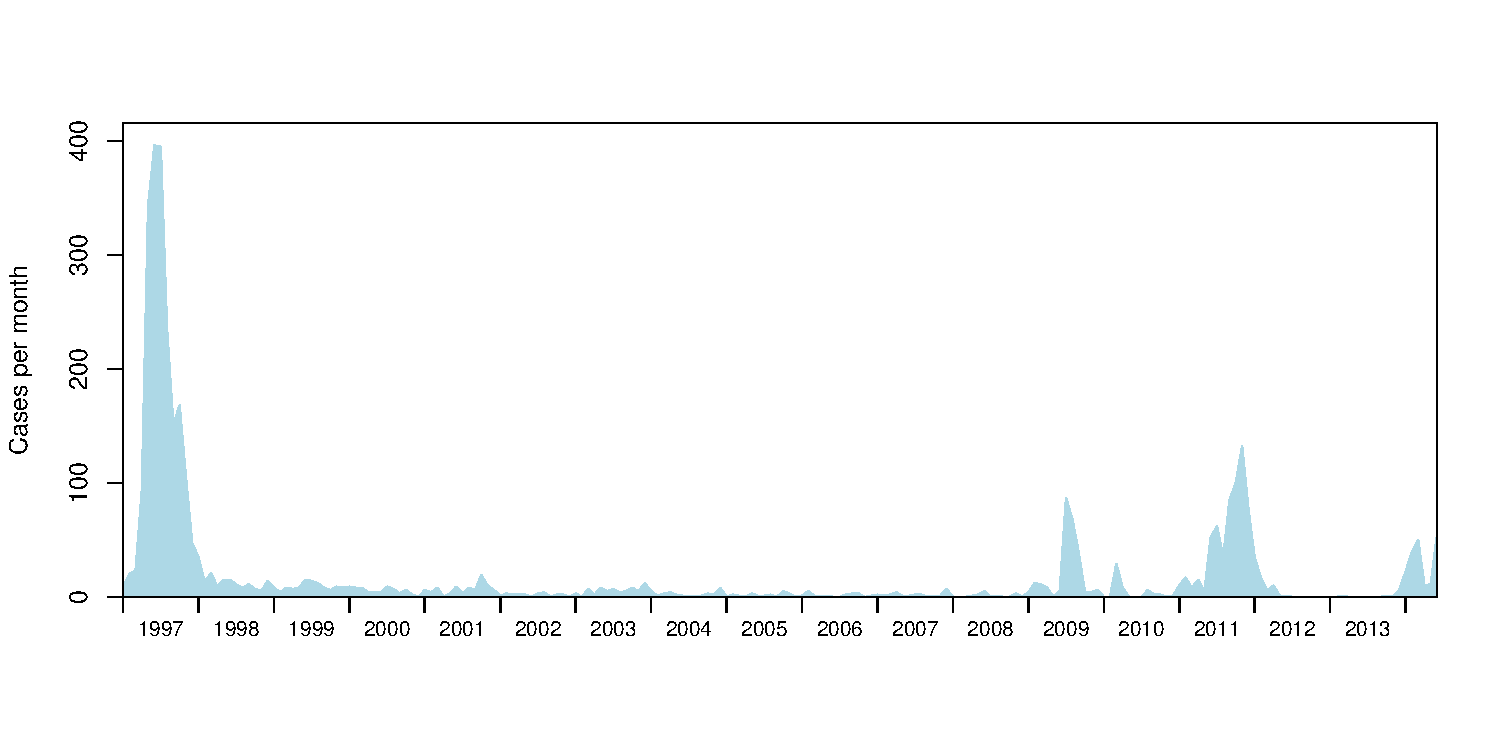
\includegraphics[width=1\textwidth]{incidence_1997_2014.pdf}
     \caption{Measles incidence from 1997 to 2014}
     \label{fig:incidence1997}
\end{figure}

In light of the apparent increasing trend in measles incidence in the last few years (Figure~\ref{fig:incidence1997}), we reviewed the information on measles importation and the origins of the introductions of measles into New Zealand. To help understand the risk of measles importation, with a particular goal of enabling the Ministry to better inform travellers and understand high risk periods, we sought to use quantitative methods to evaluate the risk of measles importation. 

\subsection{Additional risk analyses methods}

For our initial analyses, we use arrivals data from New Zealand immigration (\href{http://www.immigration.govt.nz/}{www.immigration.govt.nz}) as a proxy for human movement to and from New Zealand. We collated country population size, measles incidence and measles vaccination cover from the WHO (\href{http://www.who.int/research/en/}{www.who.int/research/en/}). Note this uses all immigration of foreign nationals, coming for whatever purpose. We used the WHO data to determine per capita measles cases for each year and used these data and the number of immigrants to New Zealand to begin to understand where measles was likely to be imported from.

%%%%%%%%%%%%%%%%%%

\begin{table}
\caption{Total travel numbers (2012)}
%latex.default(immigration, file = "", table.env = FALSE, rowname = NULL)%
\begin{center}
\begin{tabular}{lr}
\hline\hline
\multicolumn{1}{c}{country}&\multicolumn{1}{c}{immigration}\tabularnewline
\hline
Australia&$1799655$\tabularnewline
United Kingdom&$ 401737$\tabularnewline
China&$ 322076$\tabularnewline
United States&$ 316058$\tabularnewline
Fiji&$ 151443$\tabularnewline
India&$ 107618$\tabularnewline
Japan&$ 106716$\tabularnewline
Germany&$  96308$\tabularnewline
Korea, Republic of&$  87419$\tabularnewline
France&$  85948$\tabularnewline
\hline
\end{tabular}\end{center}\label{table:immigration12}
\end{table}

%%%%%%%%%%%%%%%%%%%%%

\begin{table}
\caption{Lowest national measles vaccine cover (\%, 2012)}
%latex.default(vaccinecover, file = "", table.env = FALSE, rowname = NULL)%
\begin{center}
\begin{tabular}{lr}
\hline\hline
\multicolumn{1}{c}{country}&\multicolumn{1}{c}{cover}\tabularnewline
\hline
Equatorial Guinea&$34$\tabularnewline
Somalia&$49$\tabularnewline
Lesotho&$60$\tabularnewline
Central African Republic&$65$\tabularnewline
Papua New Guinea&$67$\tabularnewline
Chad&$69$\tabularnewline
Haiti&$69$\tabularnewline
South Sudan&$70$\tabularnewline
Gabon&$71$\tabularnewline
Yemen&$71$\tabularnewline
\hline
\end{tabular}\end{center}\label{table:cover12}
\end{table}

\begin{table}
\caption{Measles incidence per million (2012)}
%latex.default(incidence, file = "", table.env = FALSE, rowname = NULL)%
\begin{center}
\begin{tabular}{lr}
\hline\hline
\multicolumn{1}{c}{country}&\multicolumn{1}{c}{incidence}\tabularnewline
\hline
Equatorial Guinea&$1617$\tabularnewline
Nauru&$1100$\tabularnewline
Democratic Republic of the Congo&$1096$\tabularnewline
Somalia&$ 979$\tabularnewline
Djibouti&$ 824$\tabularnewline
South Sudan&$ 786$\tabularnewline
Burkina Faso&$ 447$\tabularnewline
Romania&$ 342$\tabularnewline
Ukraine&$ 280$\tabularnewline
Sudan&$ 229$\tabularnewline
\hline
\end{tabular}\end{center}\label{table:incidence12}
\end{table}

\begin{table}
\caption{Risk of measles importation to New Zealand in 2012}
%latex.default(risk, file = "", table.env = FALSE, rowname = NULL)%
\begin{center}
\begin{tabular}{lr}
\hline\hline
\multicolumn{1}{c}{country}&\multicolumn{1}{c}{risk}\tabularnewline
\hline
Australia&$15537152$\tabularnewline
United Kingdom&$13386328$\tabularnewline
Thailand&$ 4774688$\tabularnewline
Malaysia&$ 4495338$\tabularnewline
Indonesia&$ 2216871$\tabularnewline
India&$ 1620172$\tabularnewline
China&$ 1432659$\tabularnewline
Ukraine&$  765096$\tabularnewline
Ireland&$  734128$\tabularnewline
Romania&$  655107$\tabularnewline
\hline
\end{tabular}\end{center}\label{table:risk12}
\end{table}



\begin{table}
\caption{Immigration numbers to New Zealand (2012)}
%latex.default(immigration, file = "", table.env = FALSE, rowname = NULL)%
\begin{center}
\begin{tabular}{lr}
\hline\hline
\multicolumn{1}{c}{country}&\multicolumn{1}{c}{immigration}\tabularnewline
\hline
Australia&$809775$\tabularnewline
United Kingdom&$306177$\tabularnewline
China&$256036$\tabularnewline
United States&$194438$\tabularnewline
Japan&$ 86676$\tabularnewline
Germany&$ 83608$\tabularnewline
Korea, Republic of&$ 73459$\tabularnewline
France&$ 71448$\tabularnewline
India&$ 69038$\tabularnewline
Canada&$ 54981$\tabularnewline
\hline
\end{tabular}\end{center}\label{table:immigration12}
\end{table}

%%%%%%%%%%%%%%%%%%%%%

\begin{table}
\caption{Lowest national measles vaccine cover (\%, 2012)}
%latex.default(vaccinecover, file = "", table.env = FALSE, rowname = NULL)%
\begin{center}
\begin{tabular}{lr}
\hline\hline
\multicolumn{1}{c}{country}&\multicolumn{1}{c}{cover}\tabularnewline
\hline
Equatorial Guinea&$34$\tabularnewline
Somalia&$49$\tabularnewline
Lesotho&$60$\tabularnewline
Central African Republic&$65$\tabularnewline
Papua New Guinea&$67$\tabularnewline
Chad&$69$\tabularnewline
Haiti&$69$\tabularnewline
South Sudan&$70$\tabularnewline
Gabon&$71$\tabularnewline
Yemen&$71$\tabularnewline
\hline
\end{tabular}\end{center}\label{table:cover12}
\end{table}

\begin{table}
\caption{Measles incidence per million (2012)}
%latex.default(incidence, file = "", table.env = FALSE, rowname = NULL)%
\begin{center}
\begin{tabular}{lr}
\hline\hline
\multicolumn{1}{c}{country}&\multicolumn{1}{c}{incidence}\tabularnewline
\hline
Equatorial Guinea&$1617$\tabularnewline
Nauru&$1100$\tabularnewline
Democratic Republic of the Congo&$1096$\tabularnewline
Somalia&$ 979$\tabularnewline
Djibouti&$ 824$\tabularnewline
South Sudan&$ 786$\tabularnewline
Burkina Faso&$ 447$\tabularnewline
Romania&$ 342$\tabularnewline
Ukraine&$ 280$\tabularnewline
Sudan&$ 229$\tabularnewline
\hline
\end{tabular}\end{center}\label{table:incidence12}
\end{table}

\begin{table}
\caption{Risk of measles importation to New Zealand in 2012}
%latex.default(risk, file = "", table.env = FALSE, rowname = NULL)%
\begin{center}
\begin{tabular}{lr}
\hline\hline
\multicolumn{1}{c}{country}&\multicolumn{1}{c}{risk}\tabularnewline
\hline
United Kingdom&$10202161$\tabularnewline
Australia&$ 6991116$\tabularnewline
Malaysia&$ 3226580$\tabularnewline
Thailand&$ 1576414$\tabularnewline
China&$ 1138900$\tabularnewline
India&$ 1039356$\tabularnewline
Indonesia&$  984022$\tabularnewline
Ukraine&$  664315$\tabularnewline
Ireland&$  585413$\tabularnewline
Romania&$  490731$\tabularnewline
\hline
\end{tabular}\end{center}\label{table:risk12}
\end{table}
%%%%%%%%%%%%%%%%%%%

\begin{table}
\caption{New Zealander travel numbers (2012)}
%latex.default(nz, file = "", table.env = FALSE, rowname = NULL)%
\begin{center}
\begin{tabular}{lr}
\hline\hline
\multicolumn{1}{c}{country}&\multicolumn{1}{c}{immigration}\tabularnewline
\hline
Australia&$989880$\tabularnewline
United States&$121620$\tabularnewline
Fiji&$104720$\tabularnewline
United Kingdom&$ 95560$\tabularnewline
Cook Islands&$ 71960$\tabularnewline
China&$ 66040$\tabularnewline
Samoa&$ 46020$\tabularnewline
Thailand&$ 41100$\tabularnewline
India&$ 38580$\tabularnewline
Canada&$ 20400$\tabularnewline
\hline
\end{tabular}\end{center}\label{table:nztravel12}
\end{table}

%%%%%%%%%%%%%%%%%%%%%

\begin{table}
\caption{Risk of measles importation to New Zealand due to New Zealand travellers in 2012}
%latex.default(nzrisk, file = "", table.env = FALSE, rowname = NULL)%
\begin{center}
\begin{tabular}{lr}
\hline\hline
\multicolumn{1}{c}{country}&\multicolumn{1}{c}{risk}\tabularnewline
\hline
Australia&$8546036$\tabularnewline
Thailand&$3198274$\tabularnewline
United Kingdom&$3184166$\tabularnewline
Malaysia&$1268758$\tabularnewline
Indonesia&$1232849$\tabularnewline
India&$ 580816$\tabularnewline
China&$ 293759$\tabularnewline
Samoa&$ 243492$\tabularnewline
Philippines&$ 241740$\tabularnewline
Nepal&$ 188450$\tabularnewline
\hline
\end{tabular}\end{center}\label{table:nzrisk12}
\end{table}

%%%%%%%%%%%%%%%%%%


%%%%%%%%%%%%%%%%%%
\subsection{Risk analyses methods}
We received the raw EpiSurv measles case data from The Institute of Environmental Science and Research Ltd (ESR) on 27 June 2014. Initial analyses of those ESR data (not shown) suggested that denominator data were required to perform multivariate analyses to avoid confounding results due to a lack of independence among risk factors. Specifically we required $\textsf{Age} \times \textsf{Prioritised Ethnicity} \times \textsf{NZDep}$ data for New Zealand to test whether interactions among case covariates provide additional information on risk over the univariate analyses performed in the \emph{Progress Towards Measles Elimination in New Zealand - Final} report. These $\textsf{Age} \times \textsf{Prioritised Ethnicity} \times \textsf{NZDep}$ data were provided to us on 3 July 2014 by the University of Otago. We used these denominator data to determine if there were interactions among specific age categories, Prioritized Ethnicities, and NZDep that might exist among cases allowing better understanding of risk of measles infection.

The University of Otago denominator data provided were not to the same detail as the ESR case data. Notably, the denominator age data were categorised into several classes: 0--5, 6--17, 18--24, 25--64, and 65+ year categories. The ethnicity denominator data were not Prioritized Ethnicity at the Level 1 Ethnic Group Codes, but at the Level 2 Ethnic Group Codes, though with some alternative codes provided that did not match the Level 2 Ethnic codes. After discussions with the University of Otago we have provided results based on the best available data, though for smaller ethnic group categories, some results may be unreliable and these are discussed below.

With the 10 NZDep classes, Prioritized Ethnicities, and the age classes above, the numerous combinations of variables led us to have 250 categories. Because for measles cases the very young appear to be disproportionately affected (Figure~\ref{fig:ageinyears}), we split the 0--5 age category into two classes, 0--2 and 3--5 years old for each of the University of Otago denominator data, assuming equal numbers of young were born into each age group over the last five years (which is supported by data from NZ statistics \citep{stats14}).


\begin{figure}[h!]
\begin{center}
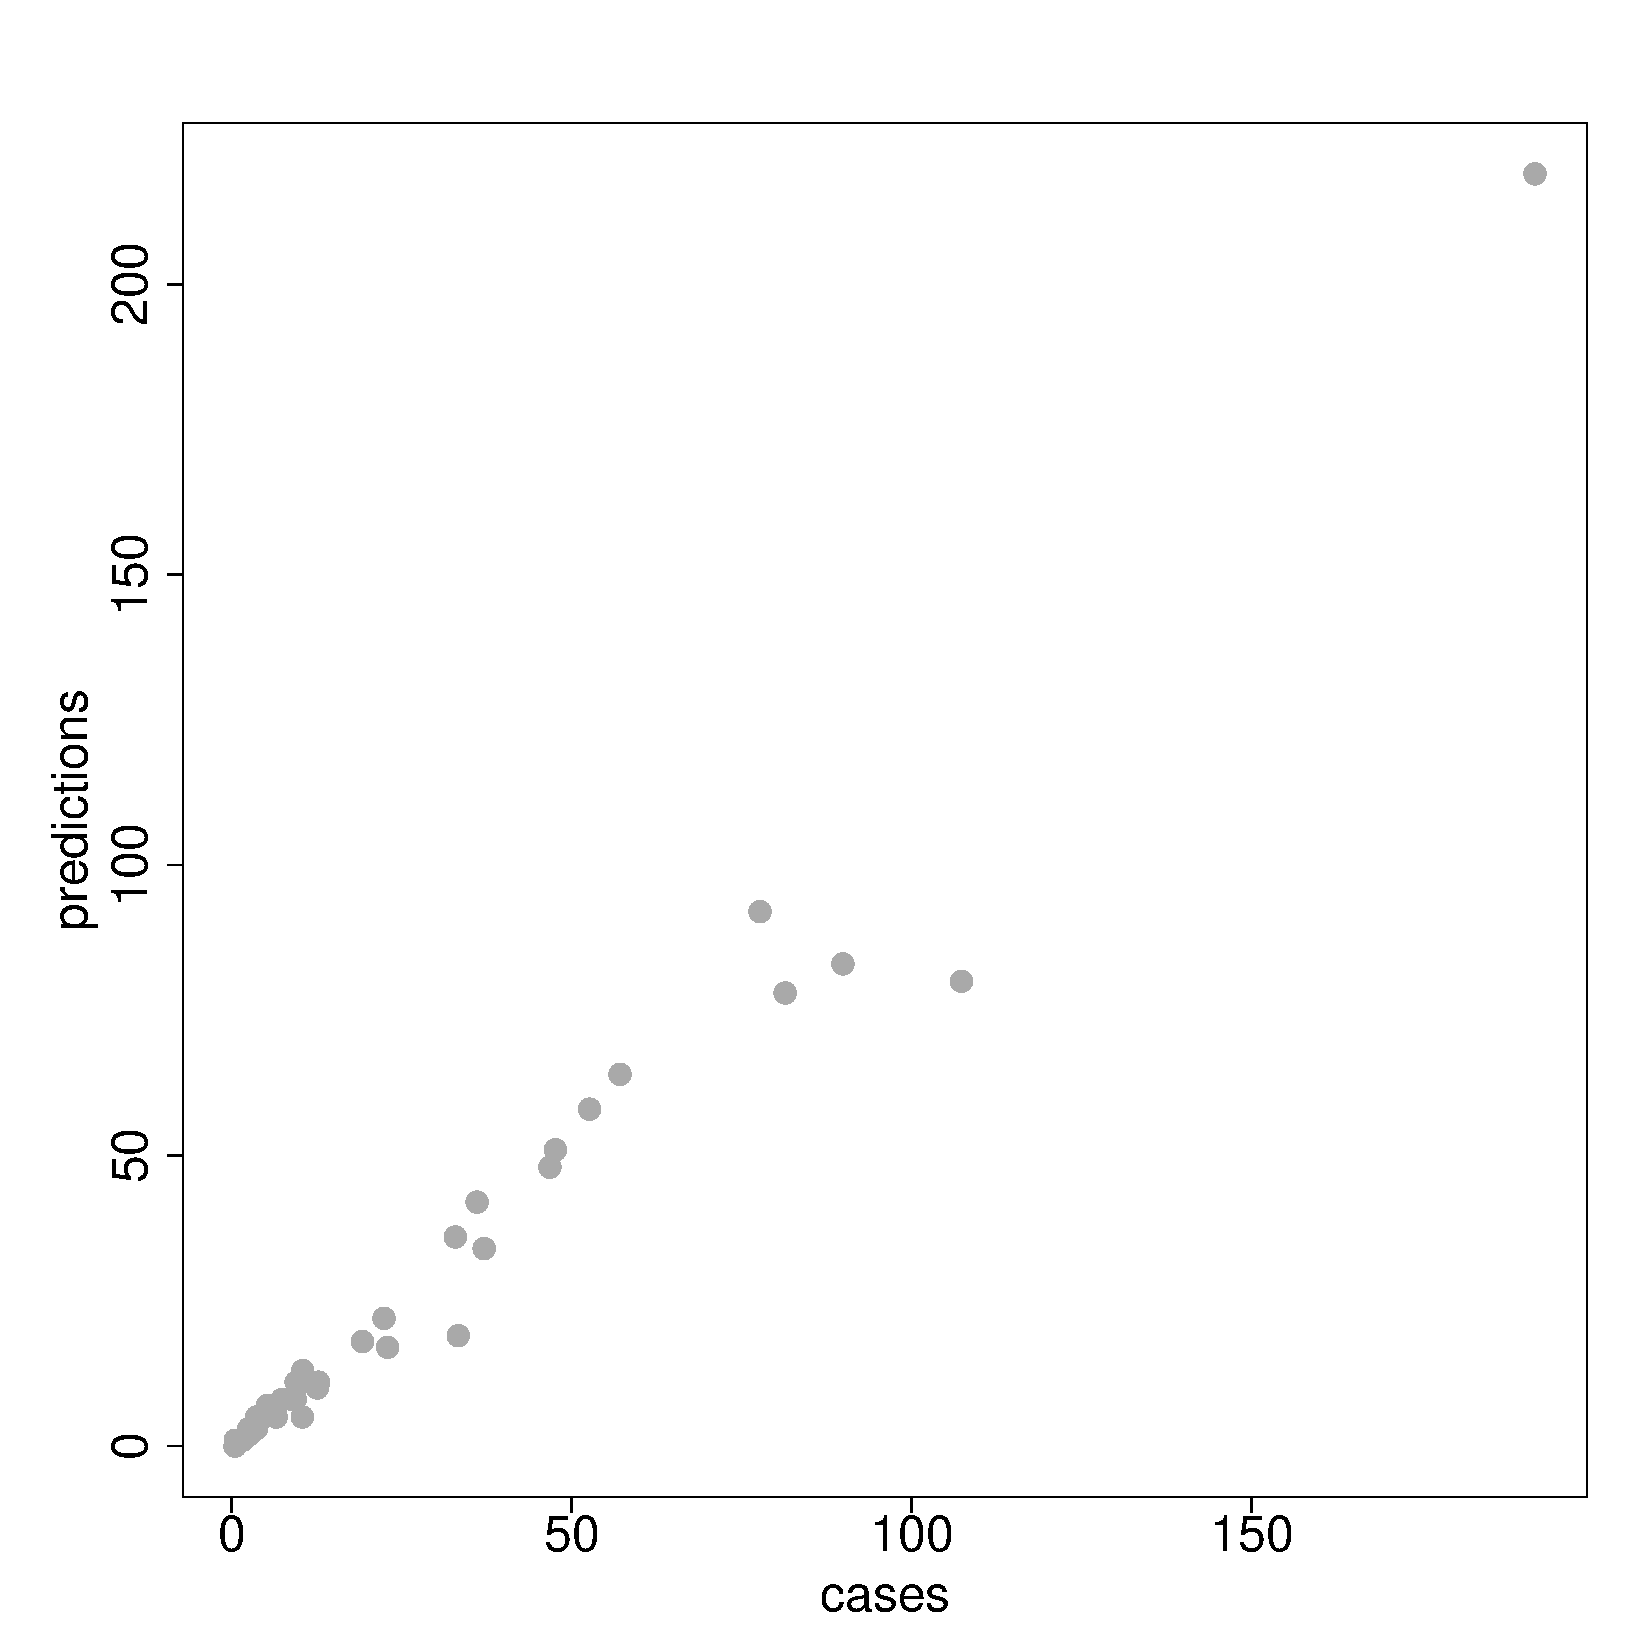
\includegraphics{draftfinalreport-015}
\end{center}
\caption{Age of measles cases in years in New Zealand for two periods, 1997--2014 and 2007--2014}
\label{fig:ageinyears}
\end{figure}





This large number of categories, some with small population sizes, lead to both overdispersion and zeroinflation, as there were many categories with zero cases in, particularly in the adult age classes. Furthermore, initial preliminary analyses, including multi-- and univariate analyses (not shown) suggested little effect of individual NZDep classifications and several higher order interactions, and therefore we reduced the number of NZDep categories from ten to two: NZDep 1--5 and NZDep 6--10. We also incorporated the 65+ age classes into the 25--64 age category, to make a 25+ age category. By doing so, we reduce the zeroinflation present in the data. 

The Prioritized Ethnicities for cases are:  European; Maori; Pacific Peoples; Asian; Middle Eastern/Latin American/African (MLA); Other Ethnicity; Residual Categories. For the analyses in this report only the first five are used, as these categories cover the overwhelming number of cases, with only 1.9\% (22/1137) of cases having no Prioritized Ethnicity (see \emph{None}, Table~\ref{table:case}). 

\begin{table}\tiny
\caption{Absolute number of measles cases in specific age, ethnicity and socio-economic deprivation categories from 2007-2014}
%latex.default(ttyr, file = "", table.env = FALSE, rowname = NULL)%
\begin{center}
\begin{tabular}{lllr}
\hline\hline
\multicolumn{1}{c}{NZDep}&\multicolumn{1}{c}{Age}&\multicolumn{1}{c}{Ethnicity}&\multicolumn{1}{c}{Cases}\tabularnewline
\hline
1-5&0-2&Asian&$ 11$\tabularnewline
6-10&0-2&Asian&$  8$\tabularnewline
1-5&3-5&Asian&$  1$\tabularnewline
1-5&6-17&Asian&$ 11$\tabularnewline
6-10&6-17&Asian&$  5$\tabularnewline
1-5&18-24&Asian&$  3$\tabularnewline
6-10&18-24&Asian&$  5$\tabularnewline
1-5&25+&Asian&$ 10$\tabularnewline
6-10&25+&Asian&$ 13$\tabularnewline
1-5&0-2&European&$ 83$\tabularnewline
6-10&0-2&European&$ 64$\tabularnewline
1-5&3-5&European&$ 42$\tabularnewline
6-10&3-5&European&$ 17$\tabularnewline
1-5&6-17&European&$219$\tabularnewline
6-10&6-17&European&$ 80$\tabularnewline
1-5&18-24&European&$ 34$\tabularnewline
6-10&18-24&European&$ 36$\tabularnewline
1-5&25+&European&$ 78$\tabularnewline
6-10&25+&European&$ 51$\tabularnewline
1-5&0-2&Maori&$ 18$\tabularnewline
6-10&0-2&Maori&$ 48$\tabularnewline
1-5&3-5&Maori&$  7$\tabularnewline
6-10&3-5&Maori&$ 11$\tabularnewline
1-5&6-17&Maori&$ 19$\tabularnewline
6-10&6-17&Maori&$ 92$\tabularnewline
1-5&18-24&Maori&$  5$\tabularnewline
6-10&18-24&Maori&$  8$\tabularnewline
1-5&25+&Maori&$  2$\tabularnewline
6-10&25+&Maori&$  6$\tabularnewline
6-10&0-2&MLA&$  3$\tabularnewline
6-10&3-5&MLA&$  1$\tabularnewline
6-10&6-17&MLA&$  1$\tabularnewline
6-10&18-24&MLA&$  2$\tabularnewline
6-10&25+&MLA&$  6$\tabularnewline
1-5&0-2&Pacific&$  5$\tabularnewline
6-10&0-2&Pacific&$ 58$\tabularnewline
6-10&3-5&Pacific&$  3$\tabularnewline
1-5&6-17&Pacific&$  5$\tabularnewline
6-10&6-17&Pacific&$ 22$\tabularnewline
1-5&18-24&Pacific&$  1$\tabularnewline
6-10&18-24&Pacific&$  8$\tabularnewline
1-5&25+&Pacific&$  2$\tabularnewline
6-10&25+&Pacific&$ 11$\tabularnewline
1-5&0-2&None&$  3$\tabularnewline
1-5&3-5&None&$  1$\tabularnewline
1-5&6-17&None&$  3$\tabularnewline
6-10&6-17&None&$  4$\tabularnewline
1-5&18-24&None&$  2$\tabularnewline
6-10&18-24&None&$  1$\tabularnewline
1-5&25+&None&$  5$\tabularnewline
6-10&25+&None&$  3$\tabularnewline
\hline
\end{tabular}\end{center}\label{table:case}
\end{table}


The numbers of cases per category and population sizes for the complete data set from 2007-2014 can be seen in Table~\ref{table:percap}. Subsequent regression analyses (not shown) also suggested that the Middle Eastern/Latin American/African category was over-- or underrepresented in per capita rates given the very small sample sizes for this classification (Figure~\ref{fig:percap}, Table~\ref{table:percap}), leading to very large standard error in regression analyses. However, there are numerous issues with the data for Middle Eastern, Latin American and African ethnicities category, and along with small population sizes (Table~\ref{table:percap}), and there several issues with estimating the denominator data for this group (University of Otago, personal communication). Thus, we removed this grouping for our subsequent analyses and are left with Asian, European, Maori and Pacific as Prioritized Ethnicities. This left us with 1102/1115 (99\%) of the measles cases with Prioritized Ethnicity recorded from 2007, and 1102/1137 (97\%) of all measles cases recorded since 2007 (Table~\ref{table:percap}).

\begin{figure}[h!]
\begin{center}
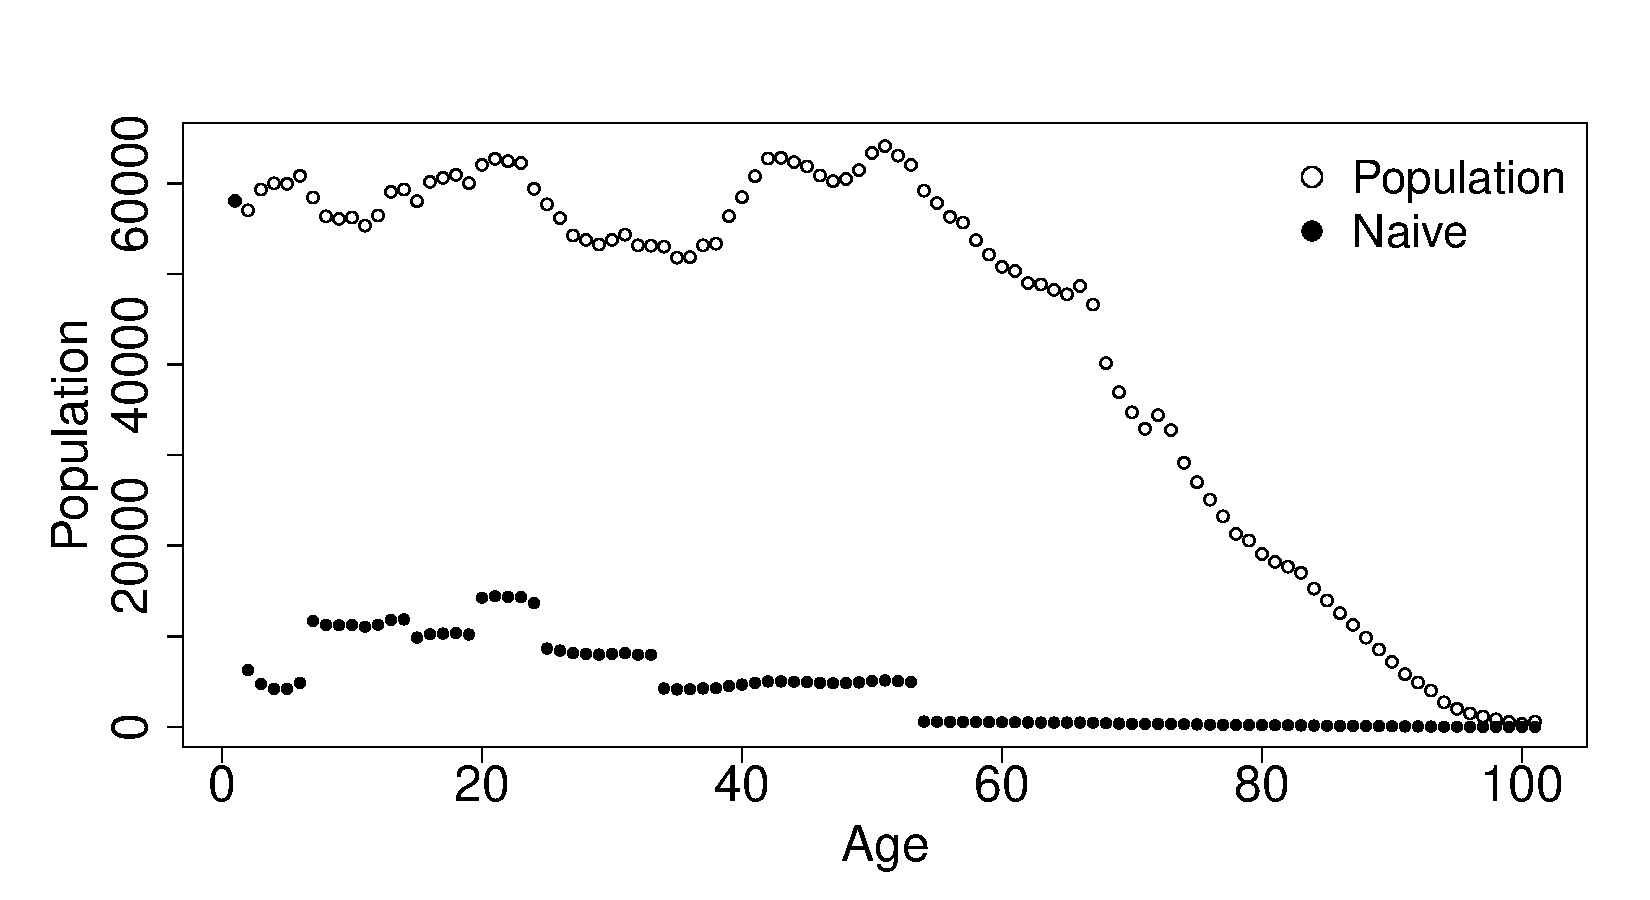
\includegraphics{draftfinalreport-023}
\end{center}
\caption{Per capita rates of measles infections broken down by ethnicity, see Table~\ref{table:percap} for details}
\label{fig:percap}
\end{figure}

\begin{table}\tiny
\caption{Numbers of measles cases, population sizes and per capita rates of measles in specific age, ethnicity and socio-economic deprivation categories from 2007-2014}
%latex.default(PerCap, file = "", table.env = FALSE, rowname = NULL)%
\begin{center}
\begin{tabular}{lllrrr}
\hline\hline
\multicolumn{1}{c}{NZDep}&\multicolumn{1}{c}{Age}&\multicolumn{1}{c}{Ethnicity}&\multicolumn{1}{c}{Population}&\multicolumn{1}{c}{Cases 1}&\multicolumn{1}{c}{Per capita}\tabularnewline
\hline
1-5&0-2&Asian&$   6094$&$ 11$&$0.0018$\tabularnewline
6-10&0-2&Asian&$   6806$&$  8$&$0.0012$\tabularnewline
1-5&3-5&Asian&$   6094$&$  1$&$0.0002$\tabularnewline
6-10&3-5&Asian&$   6806$&$  0$&$0.0000$\tabularnewline
1-5&6-17&Asian&$  33918$&$ 11$&$0.0003$\tabularnewline
6-10&6-17&Asian&$  28905$&$  5$&$0.0002$\tabularnewline
1-5&18-24&Asian&$  22917$&$  3$&$0.0001$\tabularnewline
6-10&18-24&Asian&$  34107$&$  5$&$0.0001$\tabularnewline
1-5&25+&Asian&$  96357$&$ 10$&$0.0001$\tabularnewline
6-10&25+&Asian&$  98715$&$ 13$&$0.0001$\tabularnewline
1-5&0-2&European&$  57872$&$ 83$&$0.0014$\tabularnewline
6-10&0-2&European&$  45445$&$ 64$&$0.0014$\tabularnewline
1-5&3-5&European&$  57872$&$ 42$&$0.0007$\tabularnewline
6-10&3-5&European&$  45445$&$ 17$&$0.0004$\tabularnewline
1-5&6-17&European&$ 264330$&$219$&$0.0008$\tabularnewline
6-10&6-17&European&$ 182937$&$ 80$&$0.0004$\tabularnewline
1-5&18-24&European&$ 107649$&$ 34$&$0.0003$\tabularnewline
6-10&18-24&European&$ 117840$&$ 36$&$0.0003$\tabularnewline
1-5&25+&European&$1001916$&$ 78$&$0.0001$\tabularnewline
6-10&25+&European&$ 724317$&$ 51$&$0.0001$\tabularnewline
1-5&0-2&Maori&$  10003$&$ 18$&$0.0018$\tabularnewline
6-10&0-2&Maori&$  30104$&$ 48$&$0.0016$\tabularnewline
1-5&3-5&Maori&$  10003$&$  7$&$0.0007$\tabularnewline
6-10&3-5&Maori&$  30104$&$ 11$&$0.0004$\tabularnewline
1-5&6-17&Maori&$  40461$&$ 19$&$0.0005$\tabularnewline
6-10&6-17&Maori&$ 116640$&$ 92$&$0.0008$\tabularnewline
1-5&18-24&Maori&$  15360$&$  5$&$0.0003$\tabularnewline
6-10&18-24&Maori&$  48495$&$  8$&$0.0002$\tabularnewline
1-5&25+&Maori&$  71217$&$  2$&$0.0000$\tabularnewline
6-10&25+&Maori&$ 192729$&$  6$&$0.0000$\tabularnewline
1-5&0-2&MLA&$    728$&$  0$&$0.0000$\tabularnewline
6-10&0-2&MLA&$   1290$&$  3$&$0.0023$\tabularnewline
1-5&3-5&MLA&$    728$&$  0$&$0.0000$\tabularnewline
6-10&3-5&MLA&$   1290$&$  1$&$0.0008$\tabularnewline
1-5&6-17&MLA&$   2991$&$  0$&$0.0000$\tabularnewline
6-10&6-17&MLA&$   4539$&$  1$&$0.0002$\tabularnewline
1-5&18-24&MLA&$   1710$&$  0$&$0.0000$\tabularnewline
6-10&18-24&MLA&$   3078$&$  2$&$0.0006$\tabularnewline
1-5&25+&MLA&$   8028$&$  0$&$0.0000$\tabularnewline
6-10&25+&MLA&$  10335$&$  6$&$0.0006$\tabularnewline
1-5&0-2&Pacific&$   2093$&$  5$&$0.0024$\tabularnewline
6-10&0-2&Pacific&$  13124$&$ 58$&$0.0044$\tabularnewline
1-5&3-5&Pacific&$   2093$&$  0$&$0.0000$\tabularnewline
6-10&3-5&Pacific&$  13124$&$  3$&$0.0002$\tabularnewline
1-5&6-17&Pacific&$   8541$&$  5$&$0.0006$\tabularnewline
6-10&6-17&Pacific&$  51183$&$ 22$&$0.0004$\tabularnewline
1-5&18-24&Pacific&$   3972$&$  1$&$0.0003$\tabularnewline
6-10&18-24&Pacific&$  22098$&$  8$&$0.0004$\tabularnewline
1-5&25+&Pacific&$  18492$&$  2$&$0.0001$\tabularnewline
6-10&25+&Pacific&$  91533$&$ 11$&$0.0001$\tabularnewline
\hline
\end{tabular}\end{center}\label{table:percap}
\end{table}

For all our statistical analyses (including those above not shown) we used a Poisson error structure, but in all cases there was a need to account for overdispersion and thus we used and present the results of a quasipoission regression model. We also account for differences in population sizes by using an offset term, the log(population size). We used a model simplification approach, by beginning our analyses with all terms and all interactions, and then simplifying the models through removal of non-significant higher order interaction terms. Thus, the final model that remained with all significant interaction terms had the following linear predictor:

\begin{equation} \label{eq:reg}
 log(y) = \alpha + \beta _a (x_a)+ \beta _e(x_e)+ \beta _n (x_n) + \beta _a{}_e(x_a * x_e)+ log(population)  + \epsilon
  \end{equation}
Where $\alpha$ is the intercept, $y$ cases, $_a$ age, $_e$ Prioritized Ethnicity, $_n$ NZDep, and $\epsilon$ the error term.




\subsection{Additional risk analyses results}

Preliminary analyses of 2012 data, the most complete and current year of data, suggest immigration (whether for work, pleasure, etc.) is dominated by Australia, United Kingdom, China, and the United States, as shown in Table \ref{table:immigration12}. However, vaccination coverage is lowest and measles incidence highest in less developed nations (Table \ref{table:cover12} and Table \ref{table:incidence12}). Though the precise interactions between these different risk factors are unknown, the most simple, a product of measles incidence in 2012 and immigration numbers in 2012, suggest that though immigration is lower from some Asian countries, travel from (and thus we presume to) some Asian countries also poses a high risk of measles importation to New Zealand. These data are shown in Table \ref{table:risk12}. The data for all the variables for each nation state and territories for 2012 are plotted in Figure~\ref{fig:immigration12}, Figure~\ref{fig:incidence12}, and Figure~\ref{fig:cover12} and the risk map for measles incidence and immigration in Figure~\ref{fig:risk12}.


\begin{figure}
     \centering
     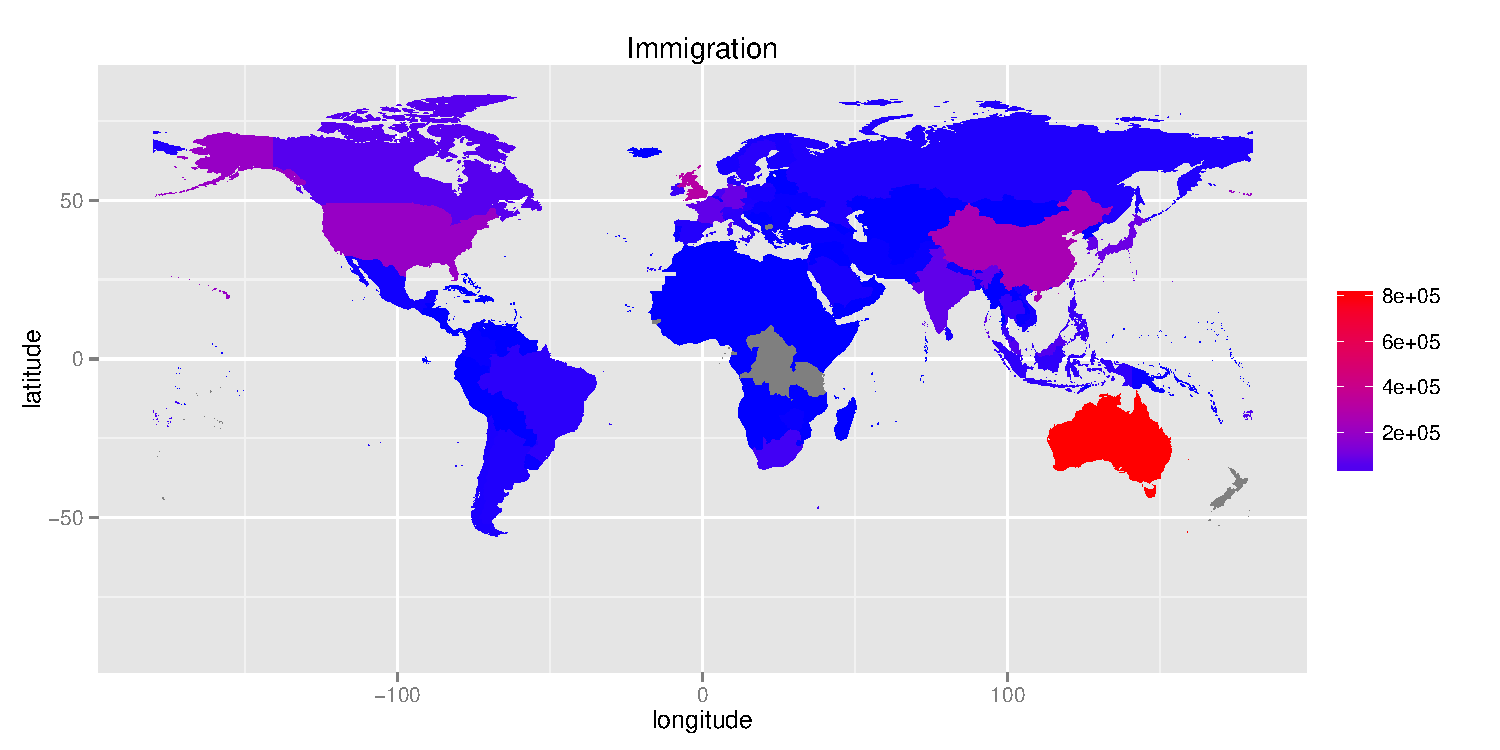
\includegraphics[width=0.8\textwidth]{np1.pdf}
     \caption{Non-New Zealander travel}
     \label{fig:immigration12}
\end{figure}

\begin{figure}
     \centering
     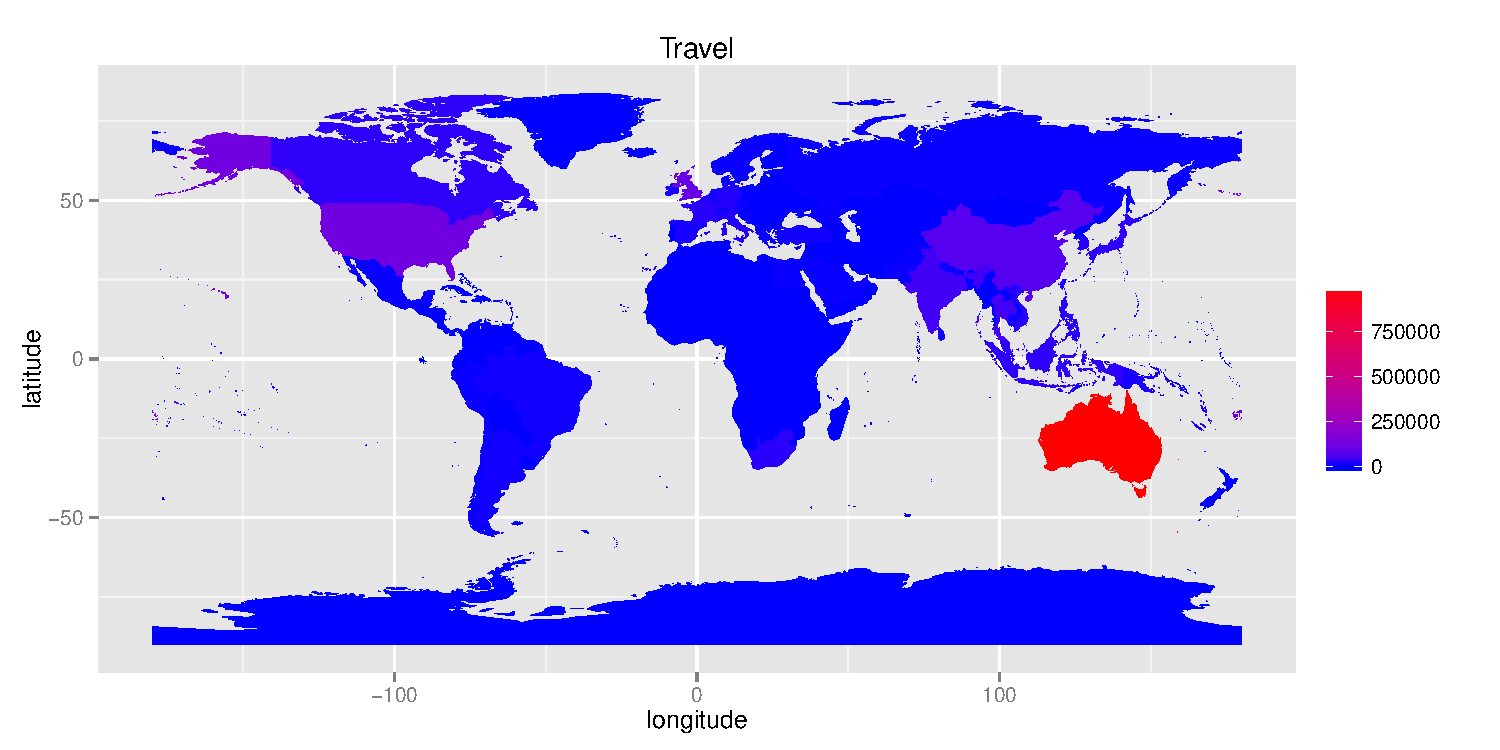
\includegraphics[width=0.8\textwidth]{nznp1.pdf}
     \caption{New Zealand travellers 2012}
     \label{fig:nztravellers}
\end{figure}

\begin{figure}
     \centering
     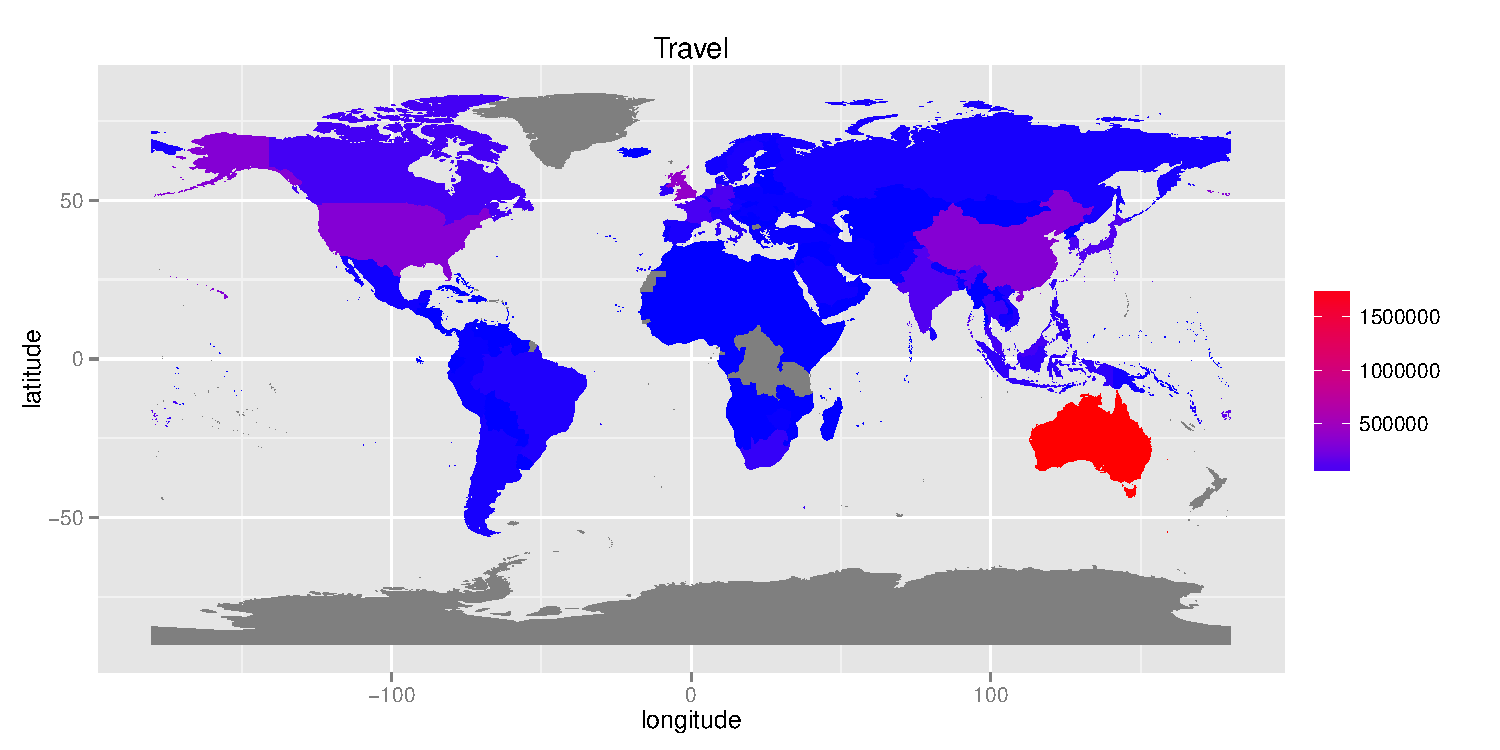
\includegraphics[width=0.8\textwidth]{totnp1.pdf}
     \caption{Total travellers 2012}
     \label{fig:tottravellers}
\end{figure}


\begin{figure}[h!]
\begin{center}
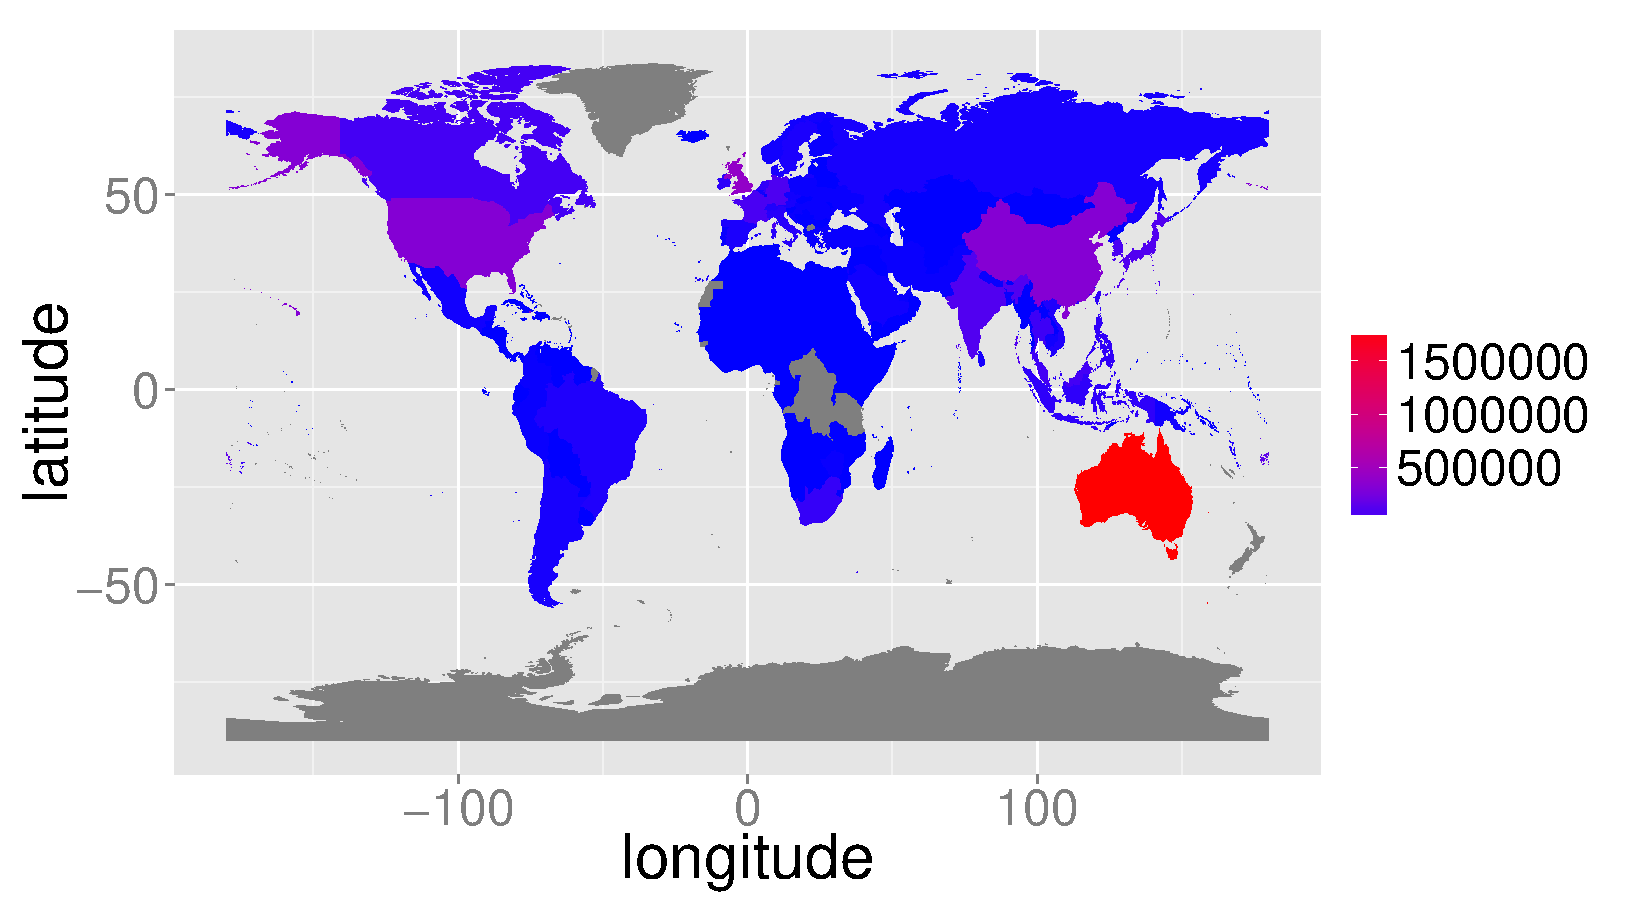
\includegraphics{draftfinalreport-028}
\end{center}
\caption{Measles incidence per million 2012}
\label{fig:incidence12}
\end{figure}

\begin{figure}[h!]
\begin{center}
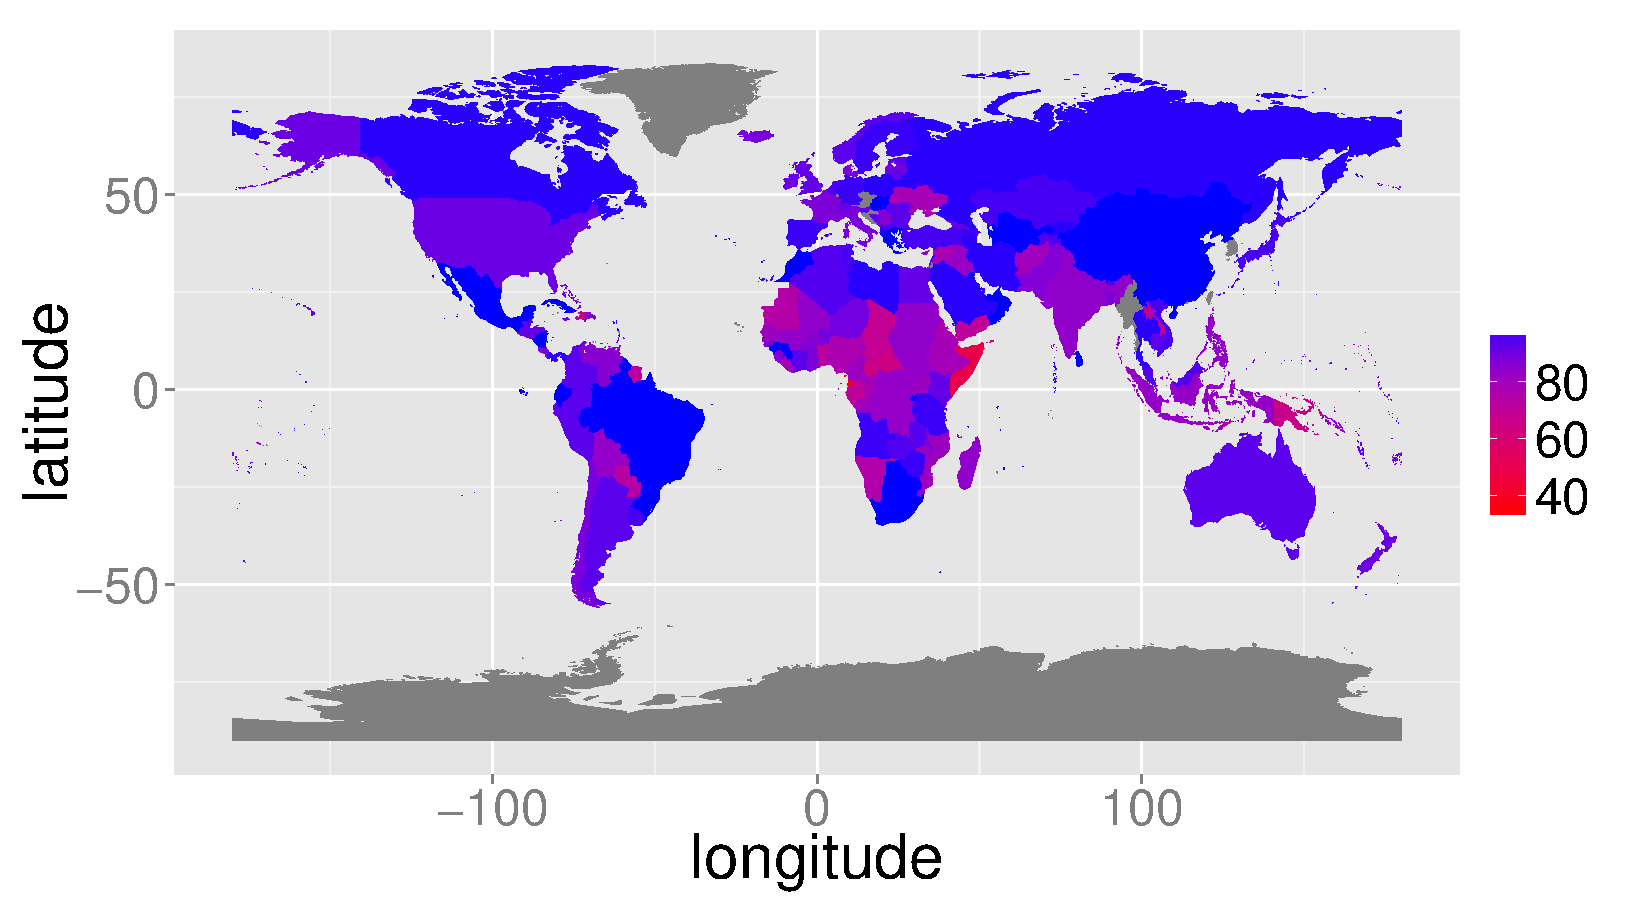
\includegraphics{draftfinalreport-029}
\end{center}
\caption{Measles vaccination cover (\%) 2012 }
\label{fig:cover12}
\end{figure}

\begin{figure}[h!]
 \centering
 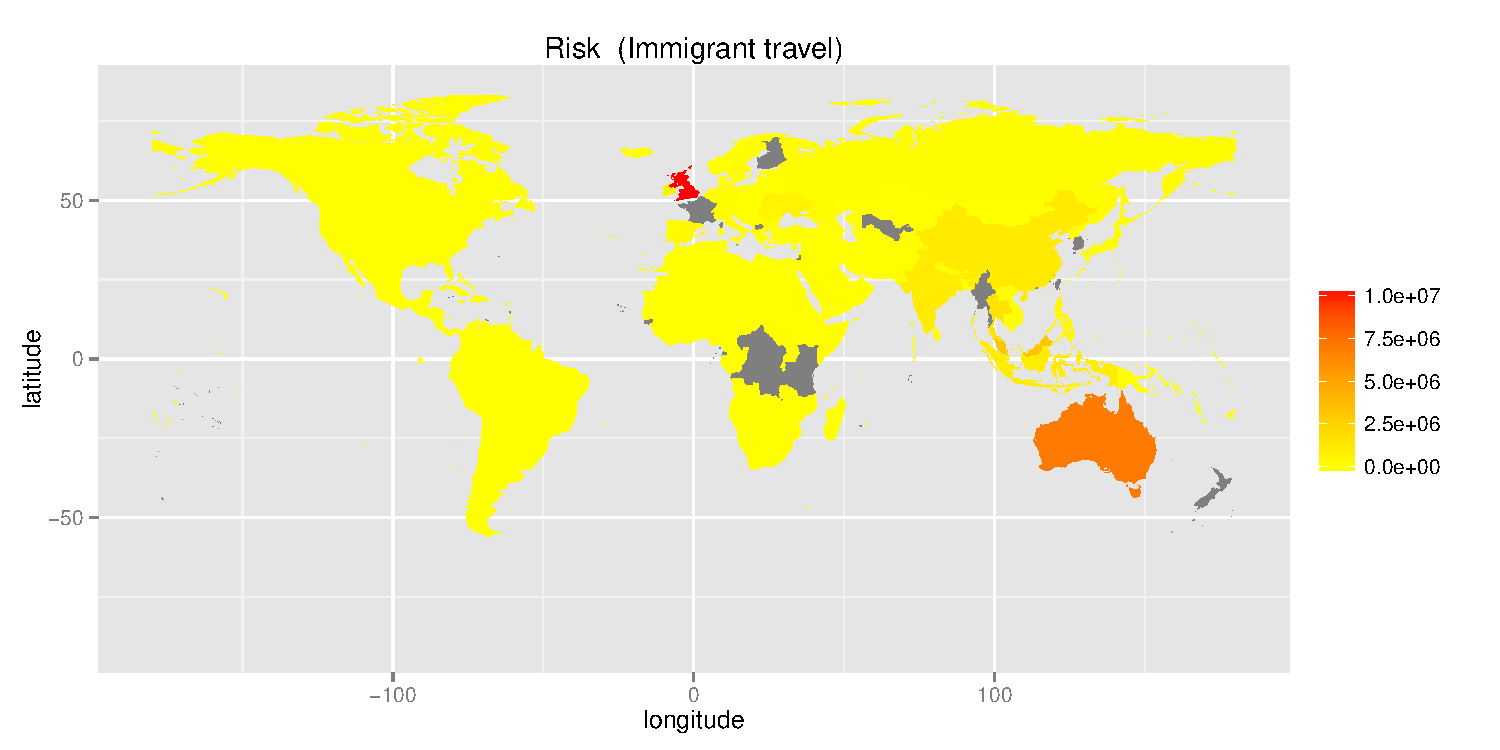
\includegraphics[width=0.8\textwidth]{np4.pdf}
\caption{Risk map from measles incidence and immigration rates}
\label{fig:risk12}
\end{figure}

\begin{figure}
     \centering
     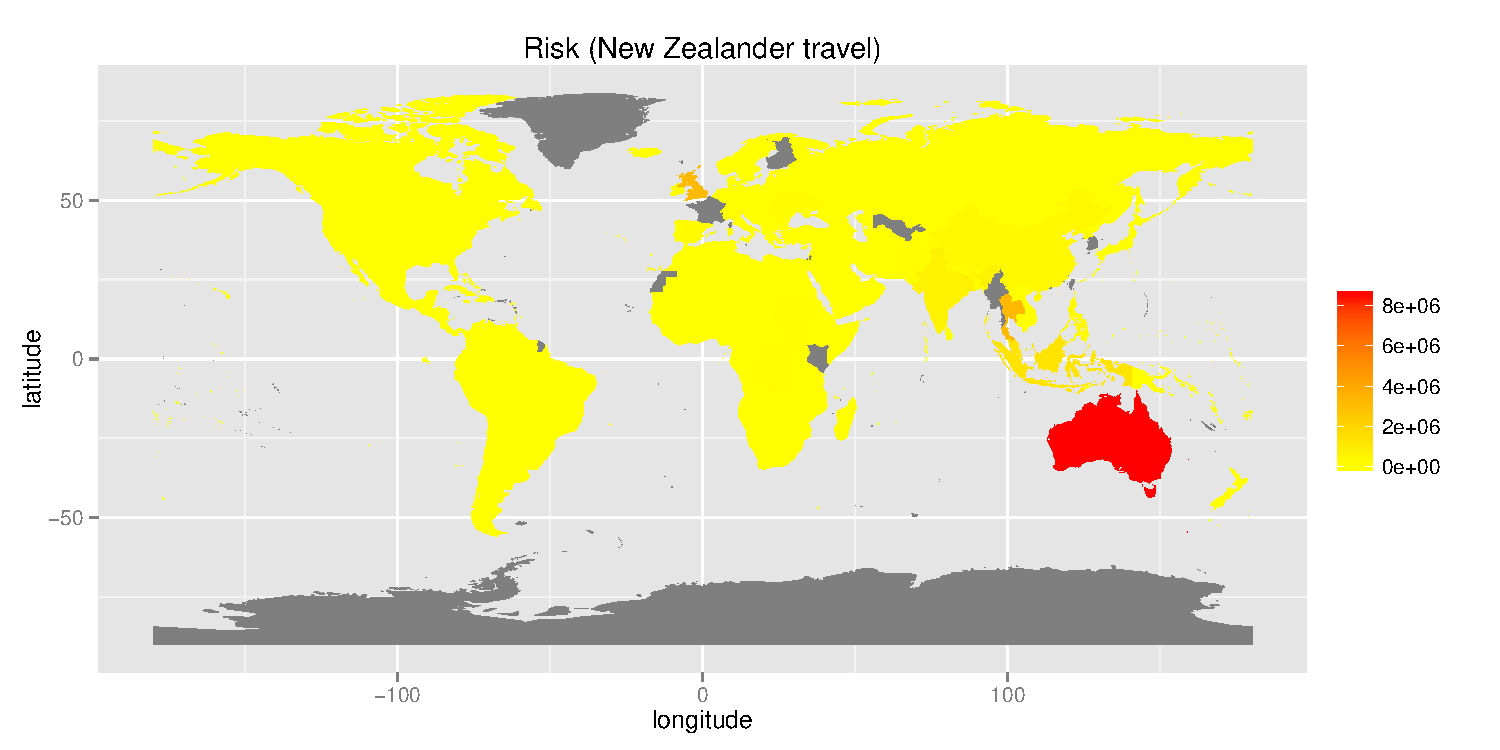
\includegraphics[width=0.8\textwidth]{nznp4.pdf}
     \caption{Risk map from measles incidence and New Zealander travel rates}
     \label{fig:nzrisk12}
\end{figure}

\begin{figure}
     \centering
     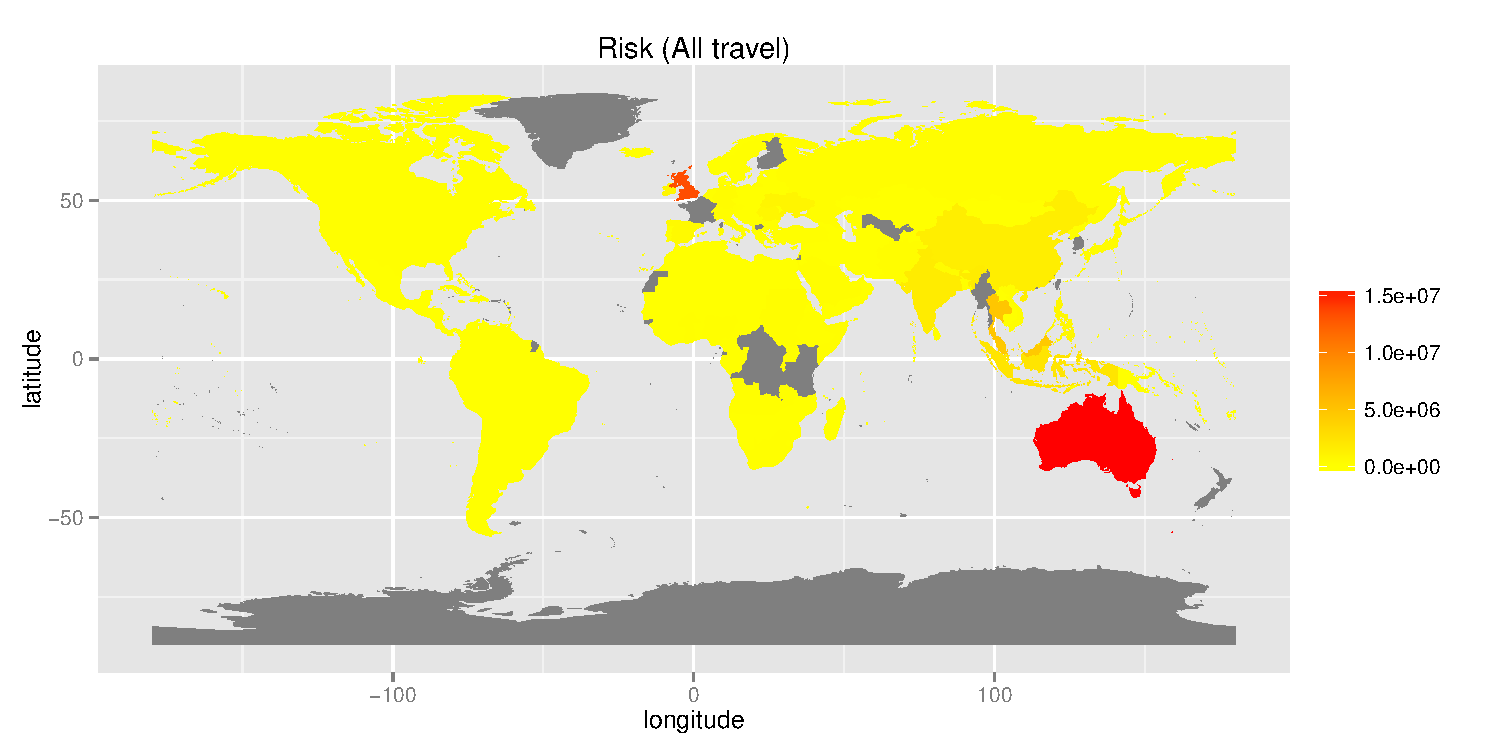
\includegraphics[width=0.8\textwidth]{totnp4.pdf}
     \caption{Risk map from measles incidence and total travel rates}
     \label{fig:totrisk12}
\end{figure}

%%%%%%%%%%% REVISE FIGURE %%%%%%%%%%%
\begin{figure}[h!]
\begin{center}
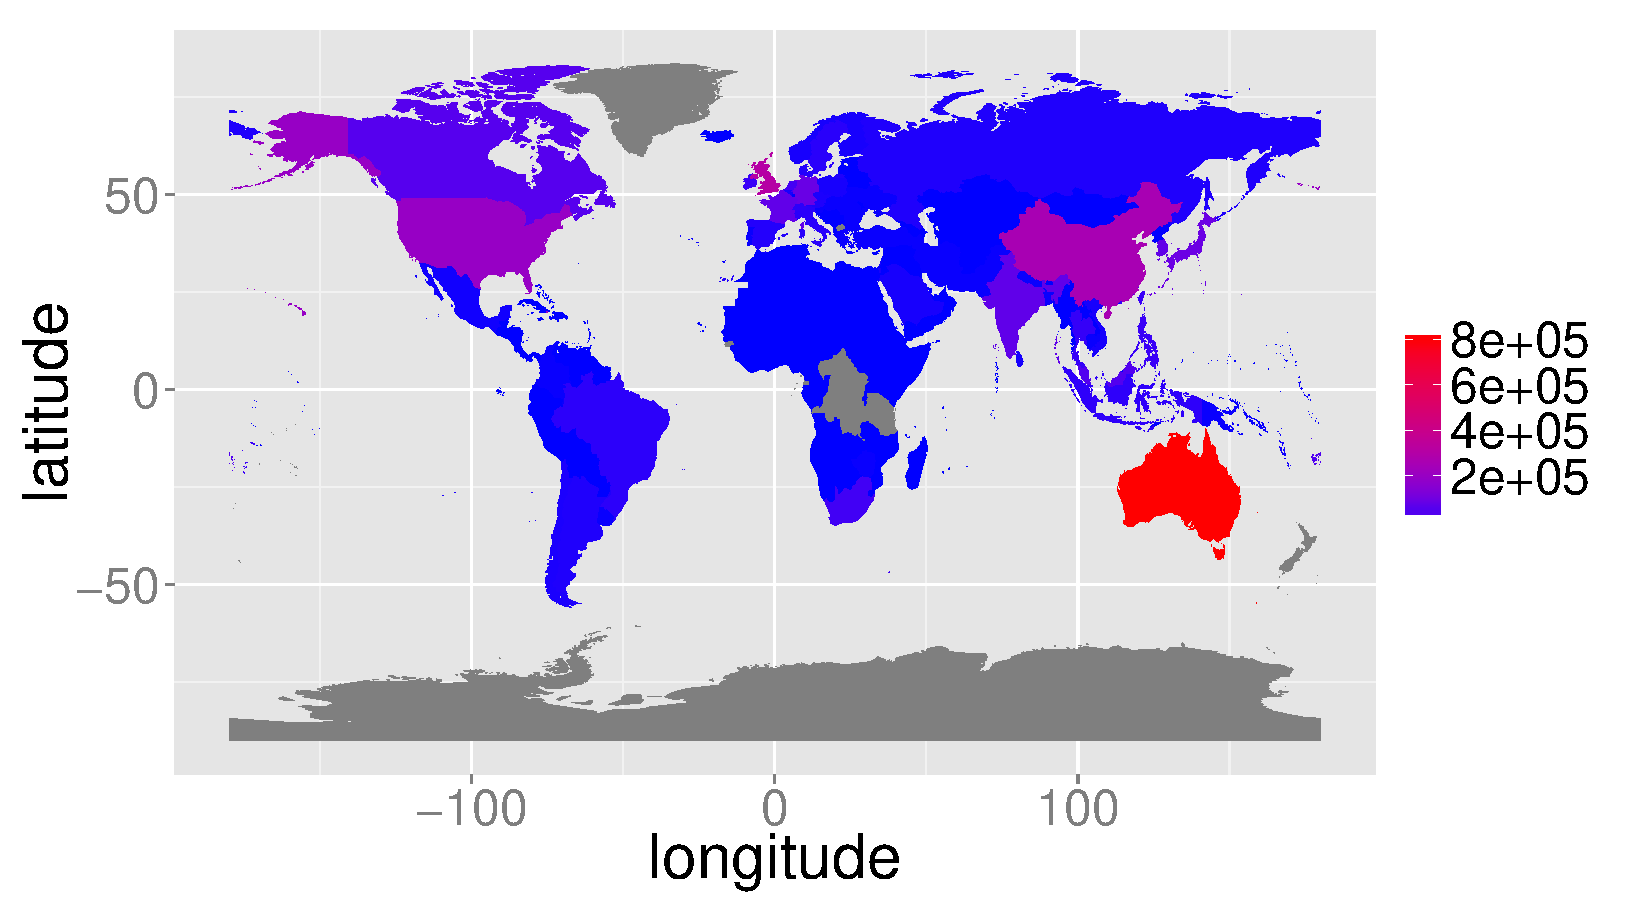
\includegraphics{draftfinalreport-030}
\end{center}
\caption{Trend in global per capita measles incidence}
\label{fig:trendincidence}
\end{figure}

\begin{figure}
     \begin{center}
     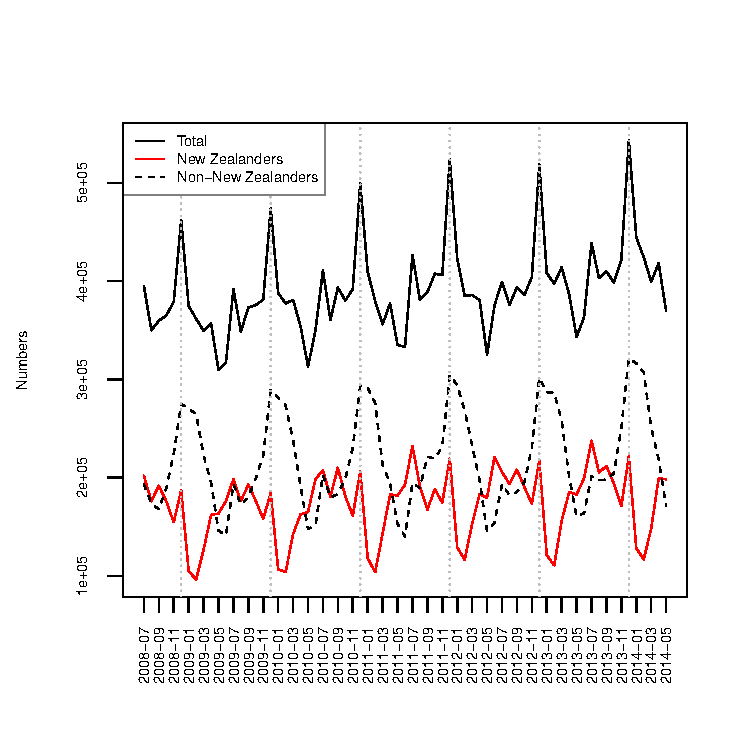
\includegraphics[width=1\textwidth]{nzers.pdf}
     \end{center}
     \caption{Trends in travel}
     \label{fig:travel}
\end{figure}

Though global incidence of measles in declining, in recent years that decline has slowed (Figure~\ref{fig:trendincidence}) and immigration rates to New Zealand have risen (Figure~\ref{fig:trendimmigration}). This suggests that the risk of measles importation could increase, though further analyses are require to understand the interaction between these variables.  Of note, however, is the clear seasonality in immigration (Figure~\ref{fig:trendimmigration}).  This seasonality suggests that there may be period of increased risk of measles importation, though again the interactions with seasonal measles transmission from the nations of origin will be an important factor in determining the risk of measles importation.

\begin{figure}[h!]
\begin{center}
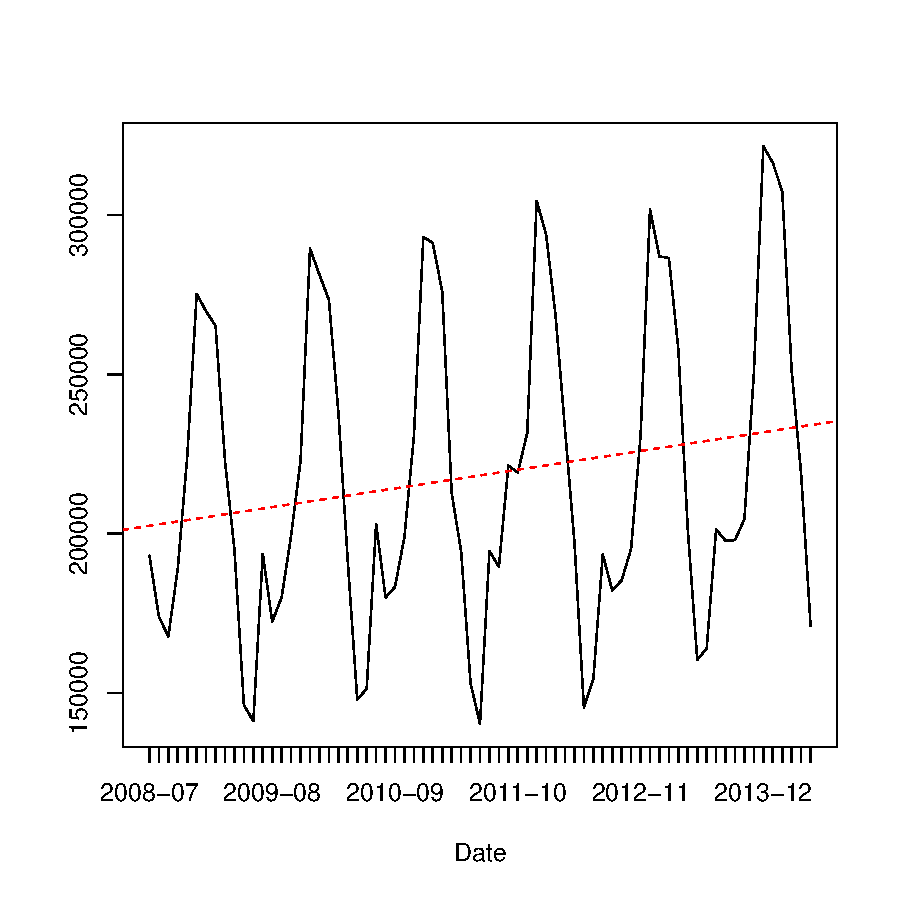
\includegraphics{draftfinalreport-031}
\end{center}
\caption{Trend in total immigrations into New Zealand}
\label{fig:trendimmigration}
\end{figure}

\begin{figure}
     \begin{center}
     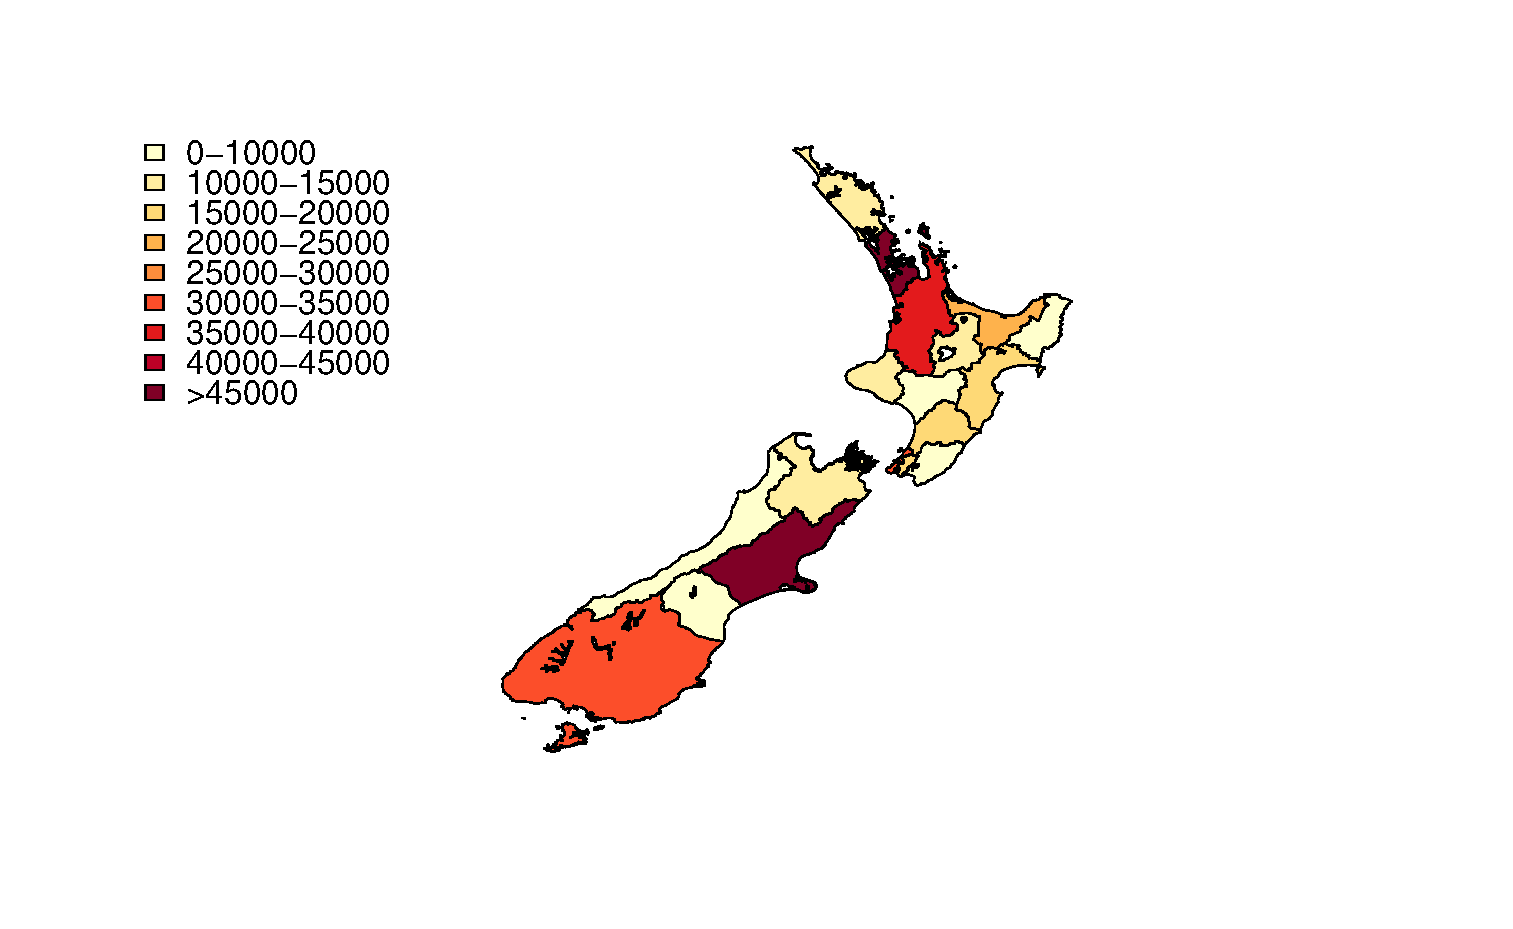
\includegraphics[width=0.6\textwidth]{naive_map.pdf}
     \end{center}
     \caption{Numbers of naive individuals per District Health Board}
     \label{fig:naive_map}
\end{figure}

\begin{figure}
     \begin{center}
     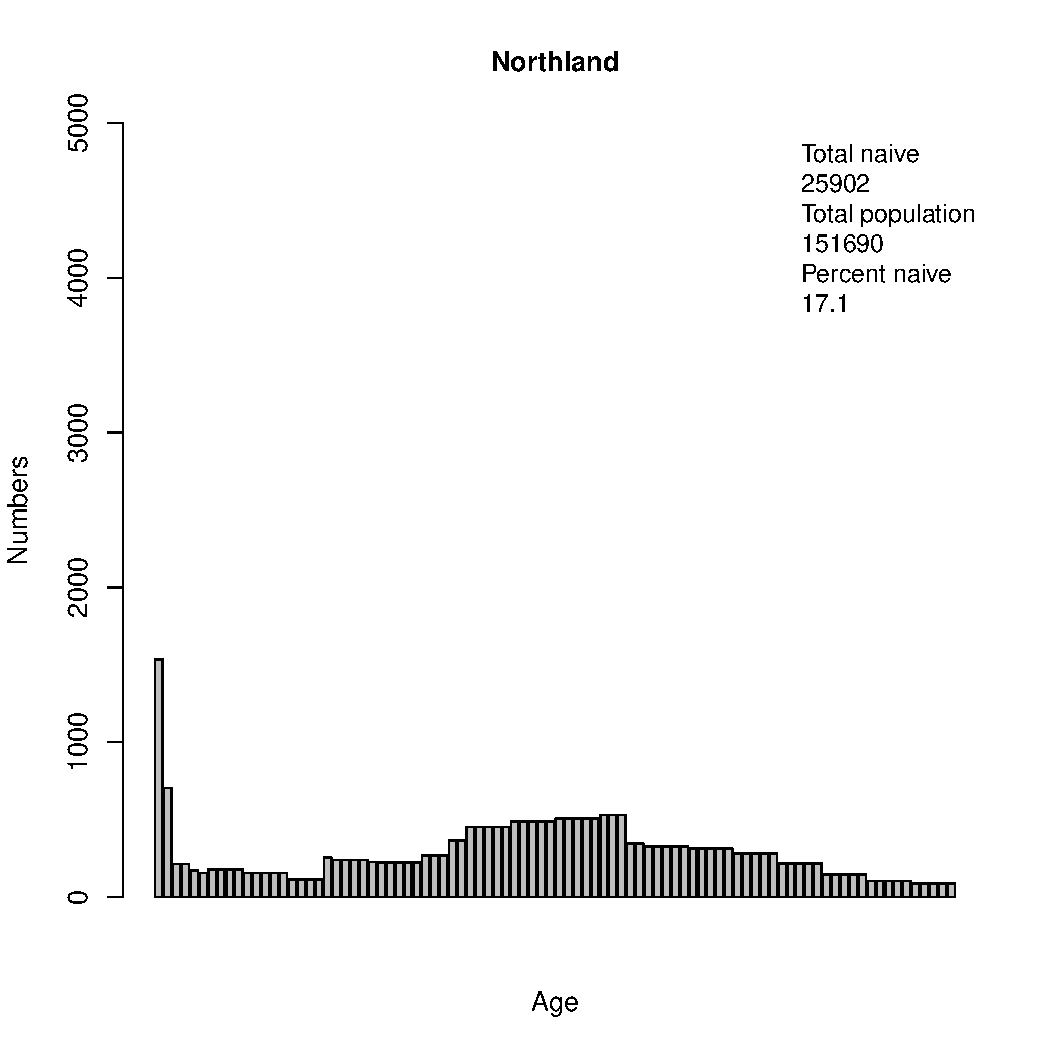
\includegraphics[width=0.6\textwidth]{dhb1.pdf}
     \end{center}
     \caption{Numbers of naive individuals per age class, Northland District Health Board}
     \label{fig:Northland}
\end{figure}


\begin{figure}
     \begin{center}
     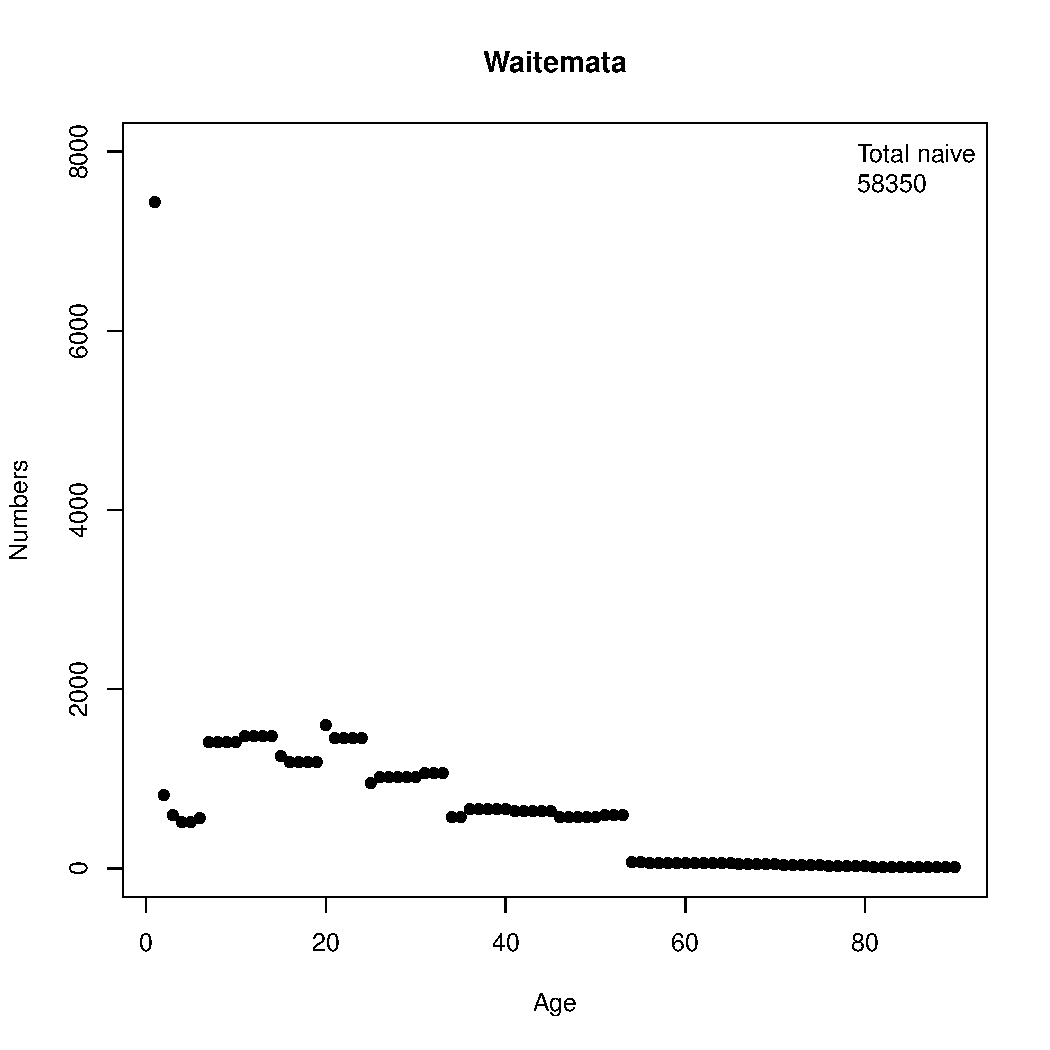
\includegraphics[width=0.6\textwidth]{dhb2.pdf}
     \end{center}
     \caption{Numbers of naive individuals per age class, Waitemata District Health Board}
     \label{fig:Waitemata}
\end{figure}

\begin{figure}
     \begin{center}
     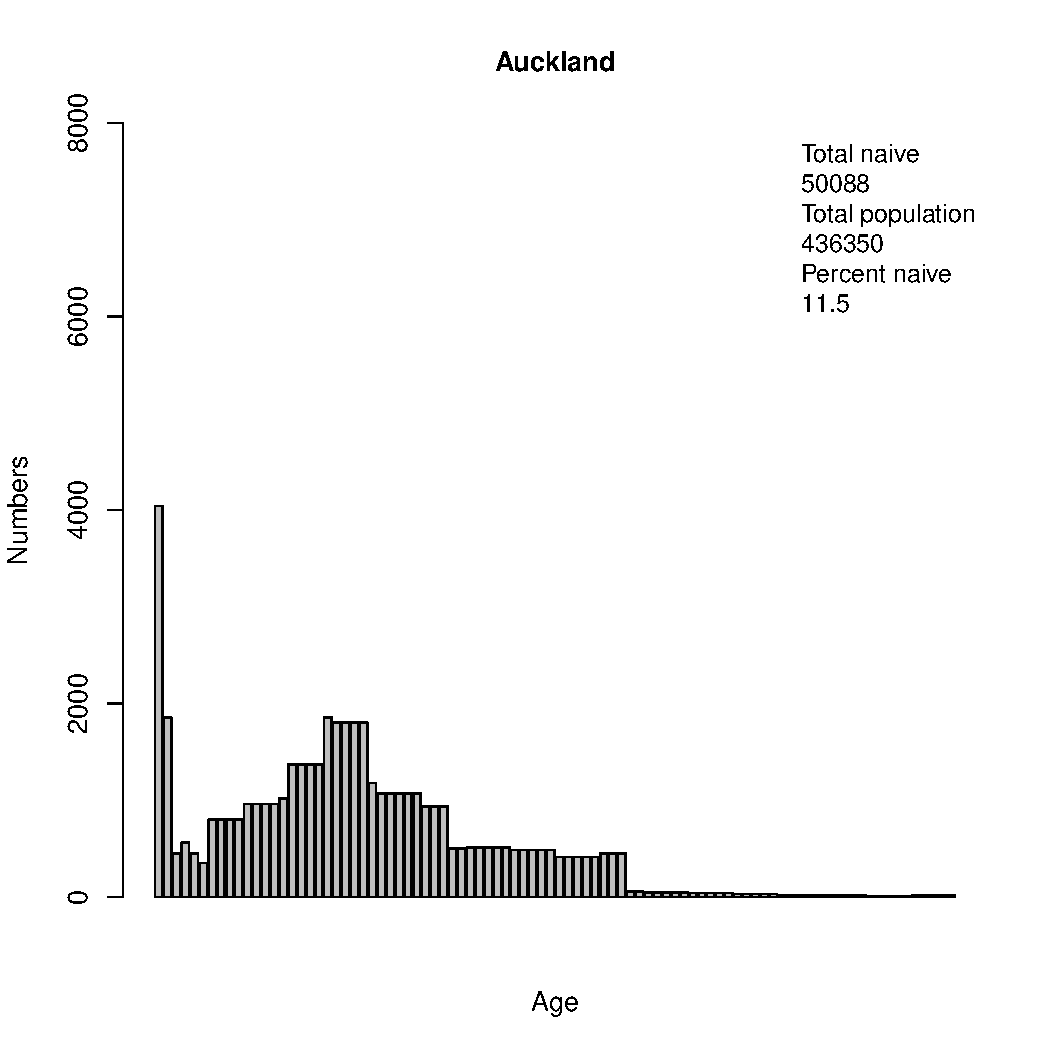
\includegraphics[width=0.6\textwidth]{dhb3.pdf}
     \end{center}
     \caption{Numbers of naive individuals per age class, Auckland District Health Board}
     \label{fig:Auckland}
\end{figure}

\begin{figure}
     \begin{center}
     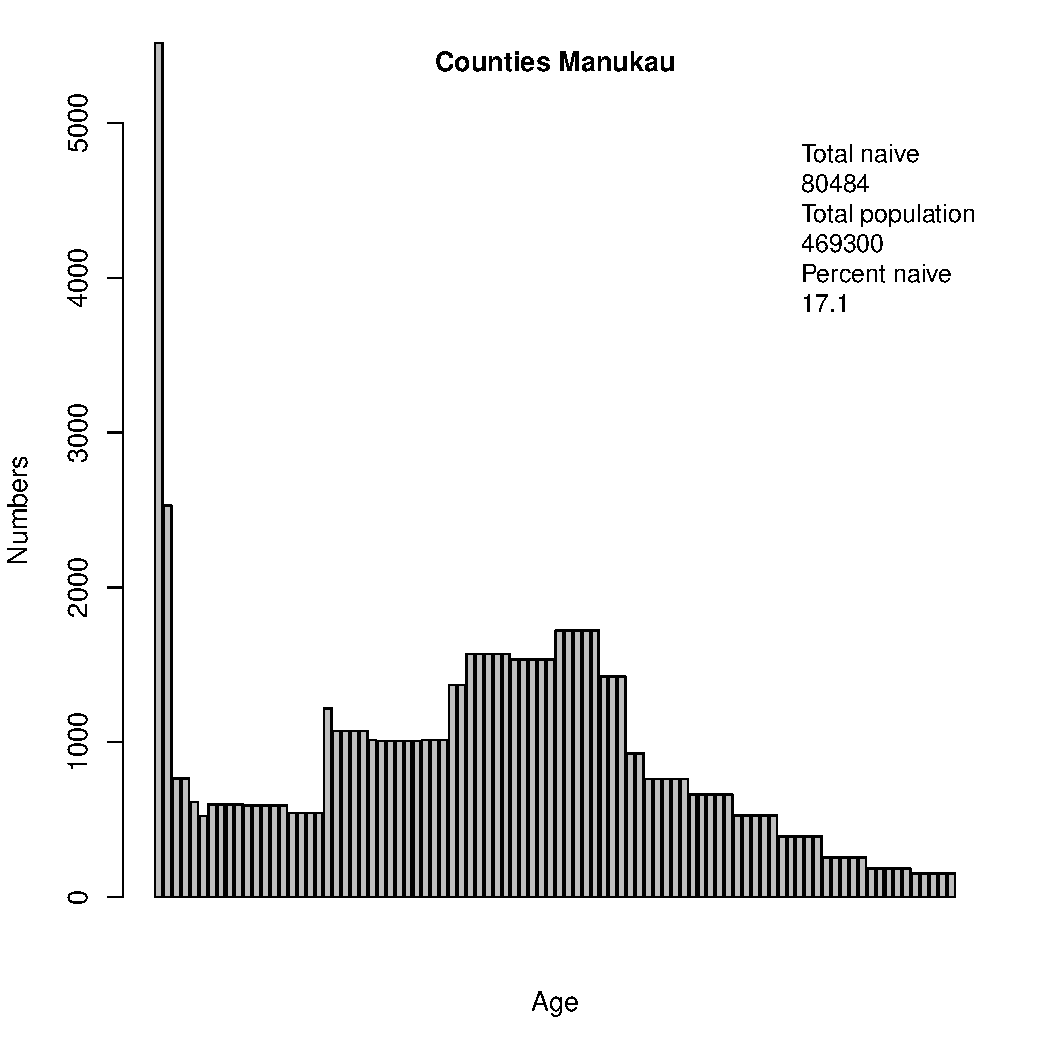
\includegraphics[width=0.6\textwidth]{dhb4.pdf}
     \end{center}
     \caption{Numbers of naive individuals per age class, Counties Manukau District Health Board}
     \label{fig:Counties_Manukau}
\end{figure}

\begin{figure}
     \begin{center}
     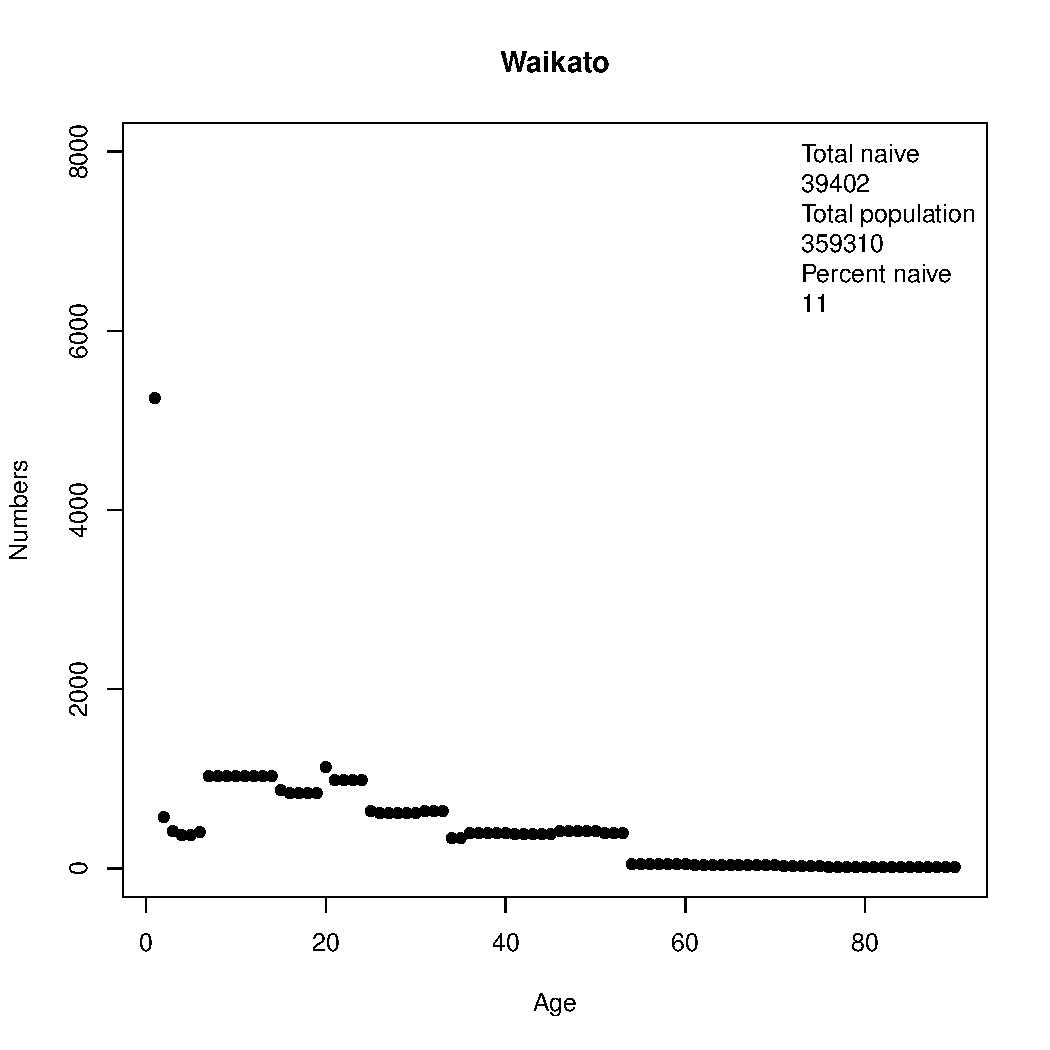
\includegraphics[width=0.6\textwidth]{dhb5.pdf}
     \end{center}
     \caption{Numbers of naive individuals per age class, Waikato District Health Board}
     \label{fig:Waikato}
\end{figure}

\begin{figure}
     \begin{center}
     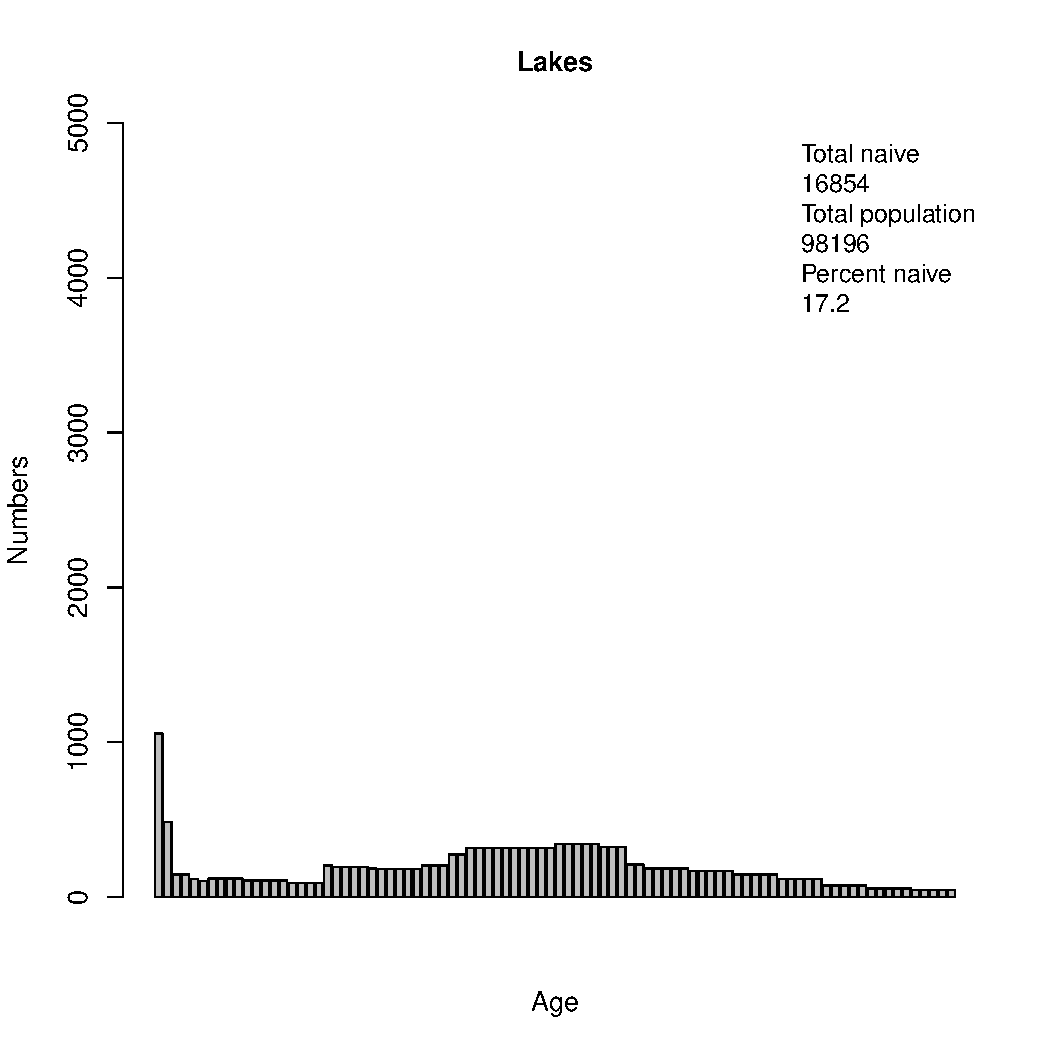
\includegraphics[width=0.6\textwidth]{dhb6.pdf}
     \end{center}
     \caption{Numbers of naive individuals per age class, Lakes District Health Board}
     \label{fig:Lakes}
\end{figure}

\begin{figure}
     \begin{center}
     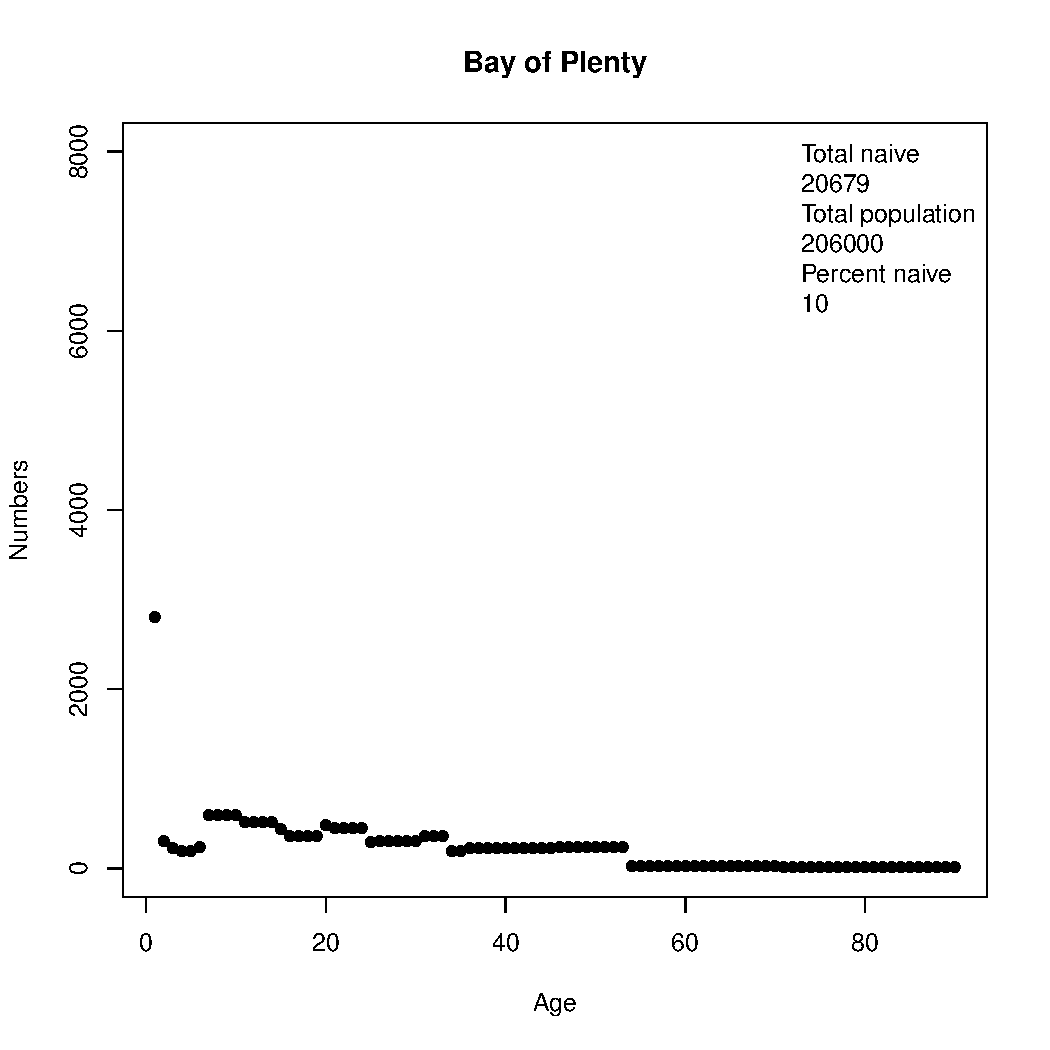
\includegraphics[width=0.6\textwidth]{dhb7.pdf}
     \end{center}
     \caption{Numbers of naive individuals per age class, Bay of Plenty District Health Board}
     \label{fig:BayofPlenty}
\end{figure}

\begin{figure}
     \begin{center}
     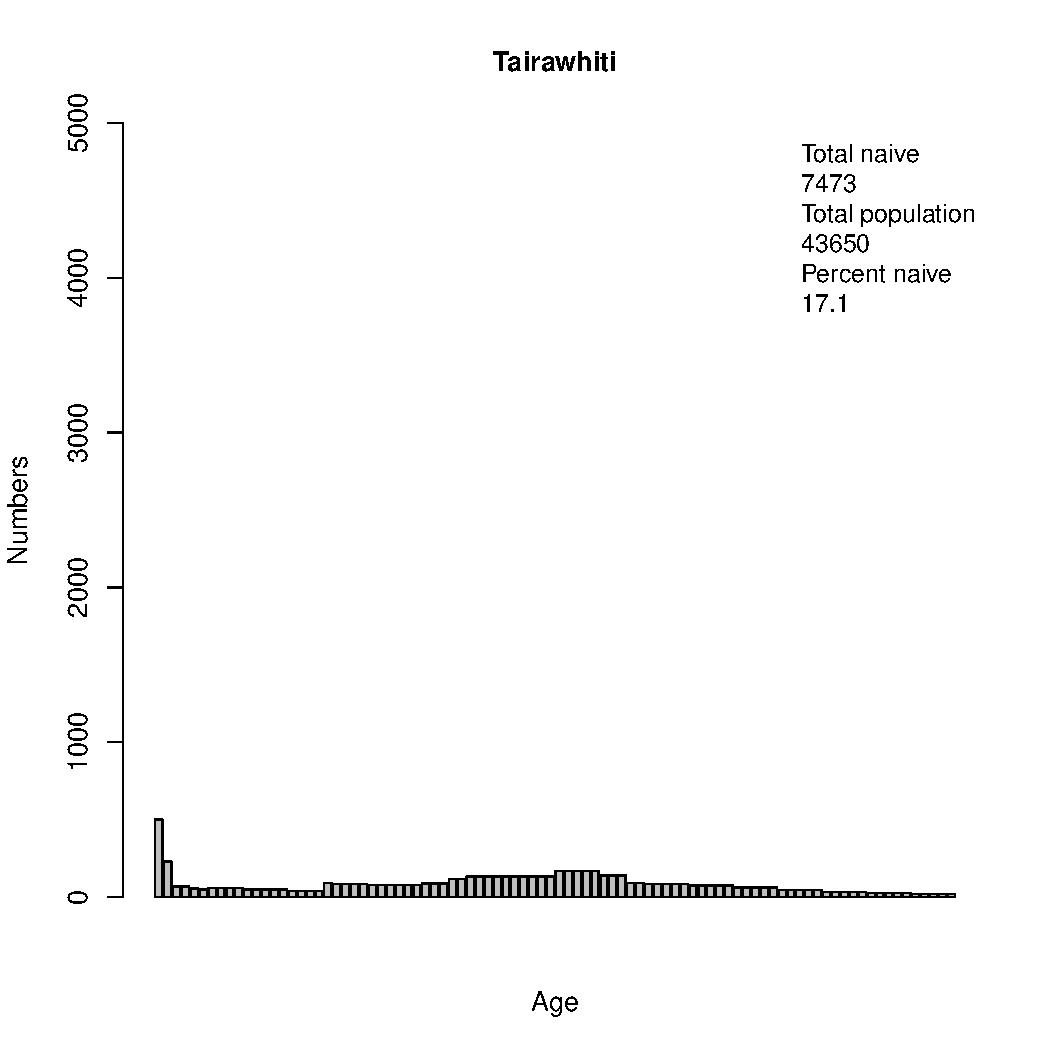
\includegraphics[width=0.6\textwidth]{dhb8.pdf}
     \end{center}
     \caption{Numbers of naive individuals per age class, Tairawhiti District Health Board}
     \label{fig:Tairawhiti}
\end{figure}

\begin{figure}
     \begin{center}
     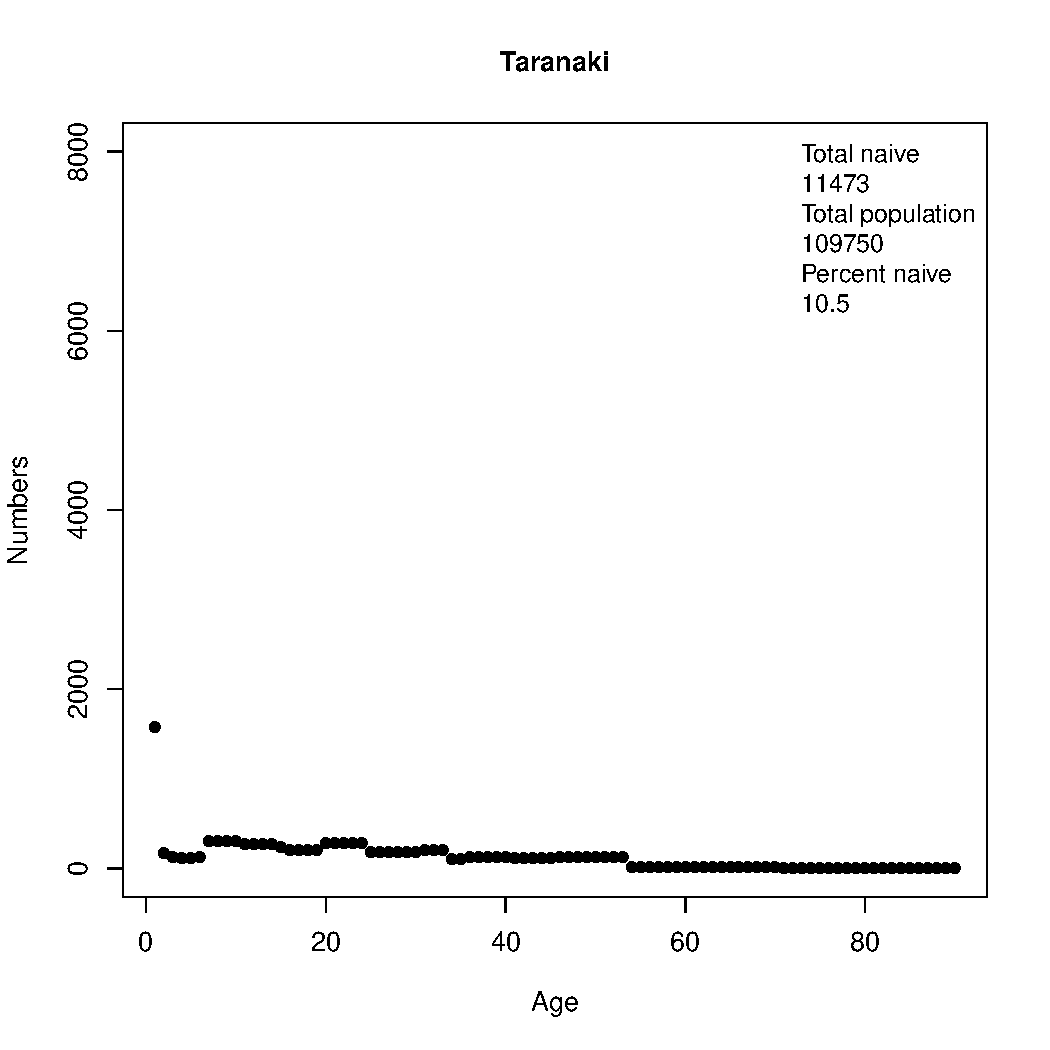
\includegraphics[width=0.6\textwidth]{dhb9.pdf}
     \end{center}
     \caption{Numbers of naive individuals per age class, Taranaki District Health Board}
     \label{fig:Taranaki}
\end{figure}

\begin{figure}
     \begin{center}
     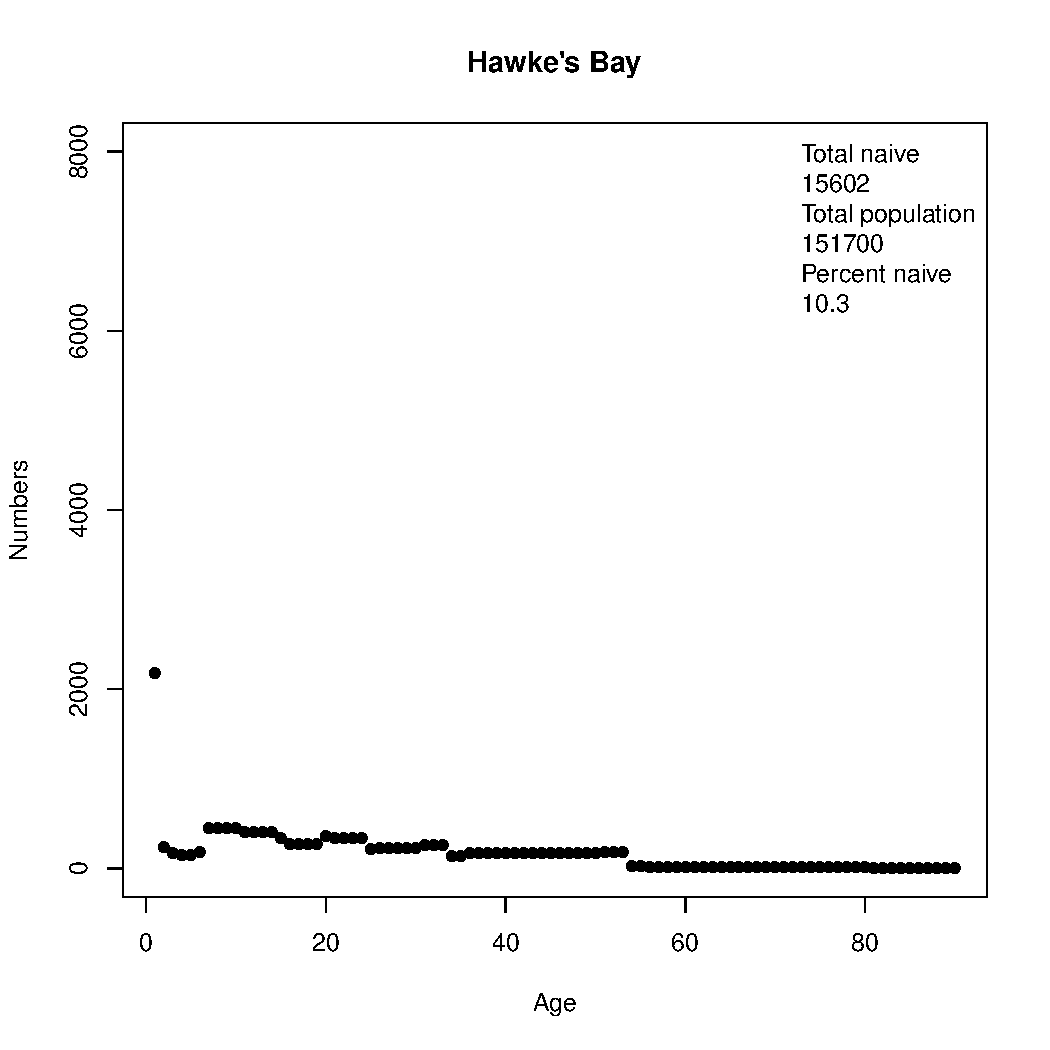
\includegraphics[width=0.6\textwidth]{dhb10.pdf}
     \end{center}
     \caption{Numbers of naive individuals per age class, Hawke's Bay District Health Board}
     \label{fig:HawkesBay}
\end{figure}

\begin{figure}
     \begin{center}
     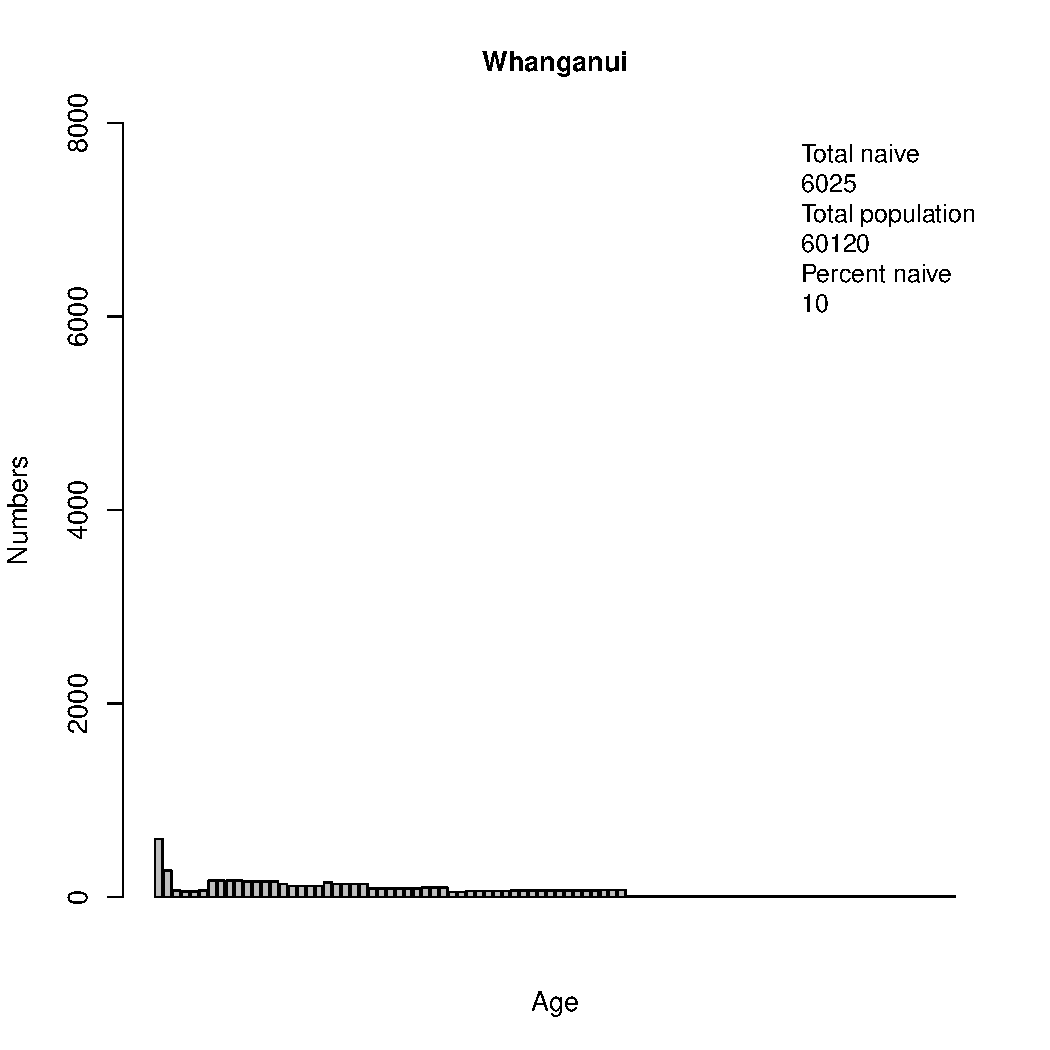
\includegraphics[width=0.6\textwidth]{dhb11.pdf}
     \end{center}
     \caption{Numbers of naive individuals per age class, Whanganui District Health Board}
     \label{fig:Whanganui}
\end{figure}

\begin{figure}
     \begin{center}
     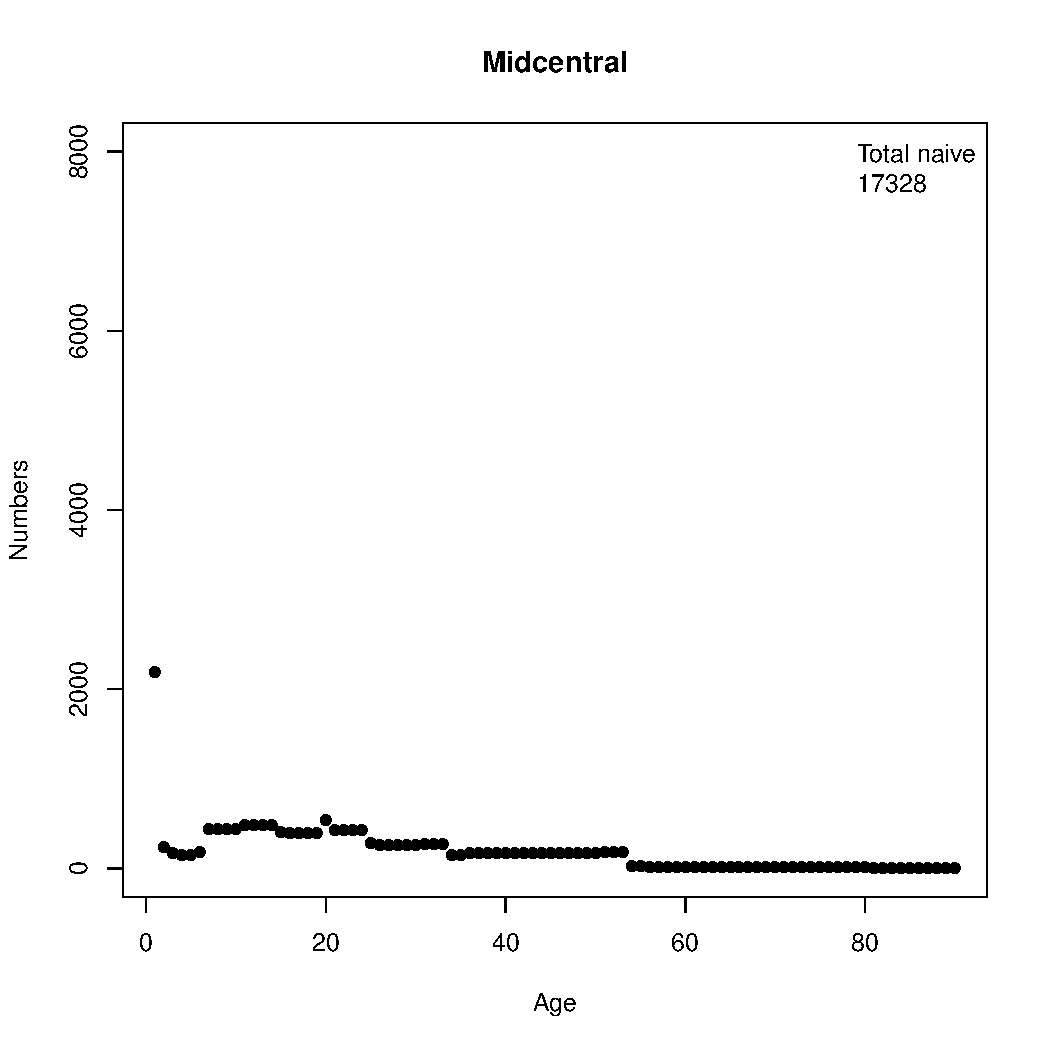
\includegraphics[width=0.6\textwidth]{dhb12.pdf}
     \end{center}
     \caption{Numbers of naive individuals per age class, Midcentral District Health Board}
     \label{fig:Midcentral}
\end{figure}

\begin{figure}
     \begin{center}
     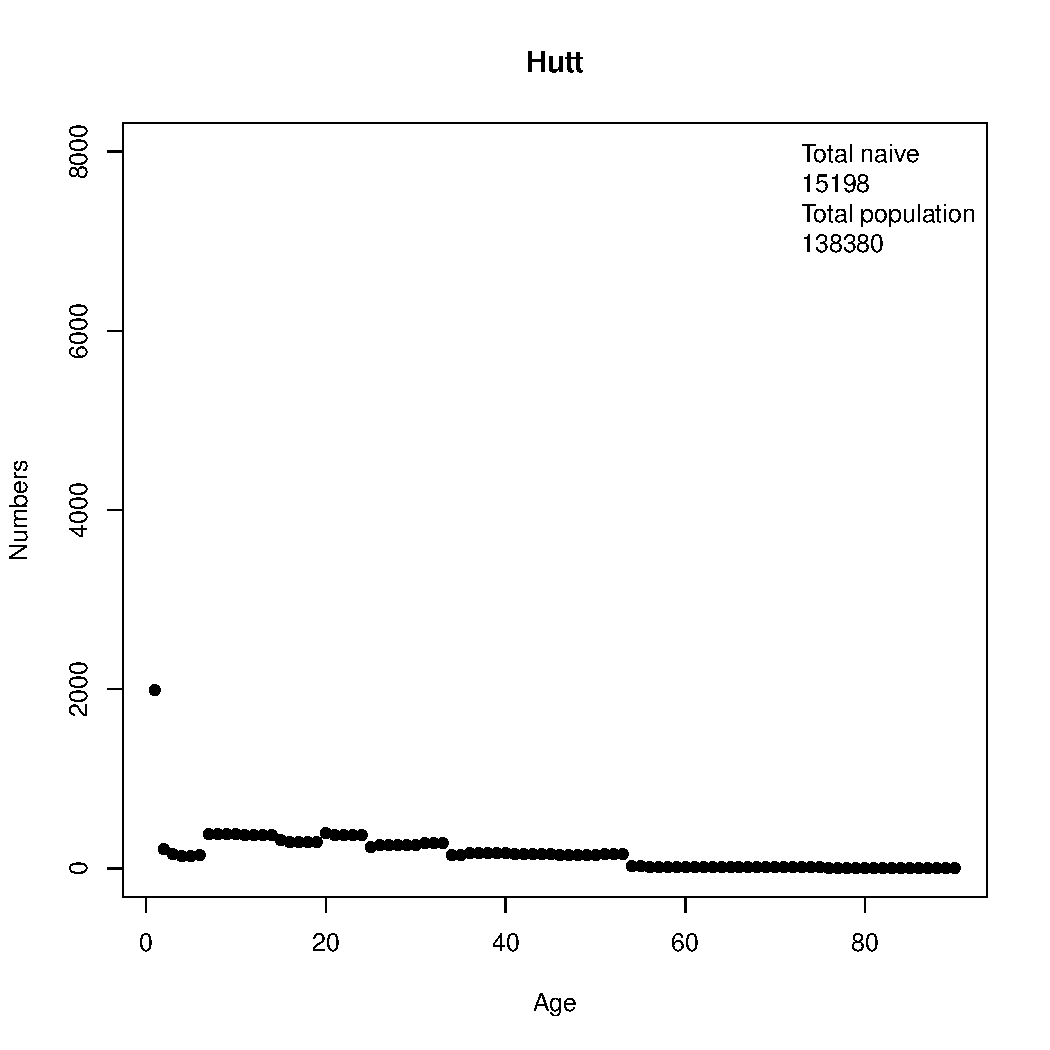
\includegraphics[width=0.6\textwidth]{dhb13.pdf}
     \end{center}
     \caption{Numbers of naive individuals per age class, Hutt District Health Board}
     \label{fig:Hutt}
\end{figure}

\begin{figure}
     \begin{center}
     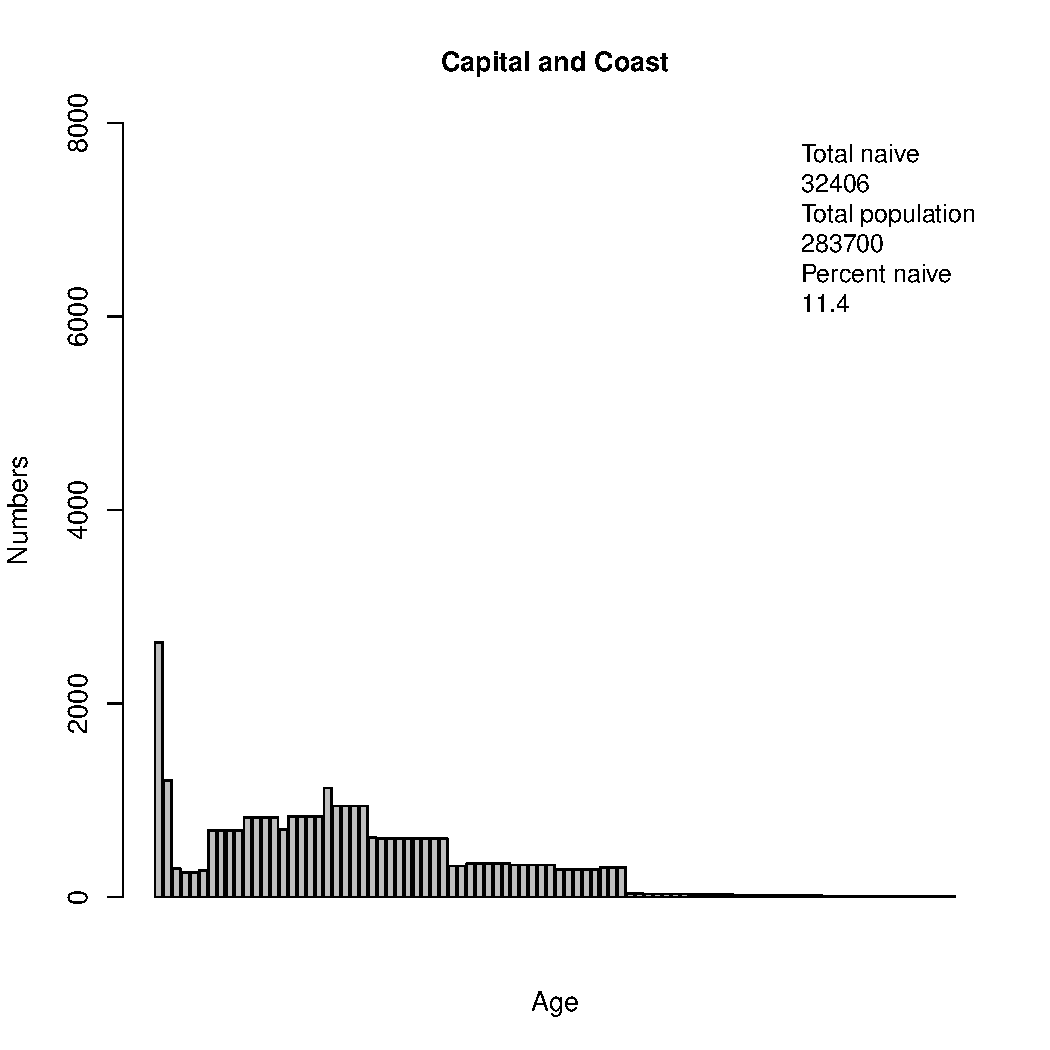
\includegraphics[width=0.6\textwidth]{dhb14.pdf}
     \end{center}
     \caption{Numbers of naive individuals per age class, Capital and Coast District Health Board}
     \label{fig:CapitalandCoast}
\end{figure}

\begin{figure}
     \begin{center}
     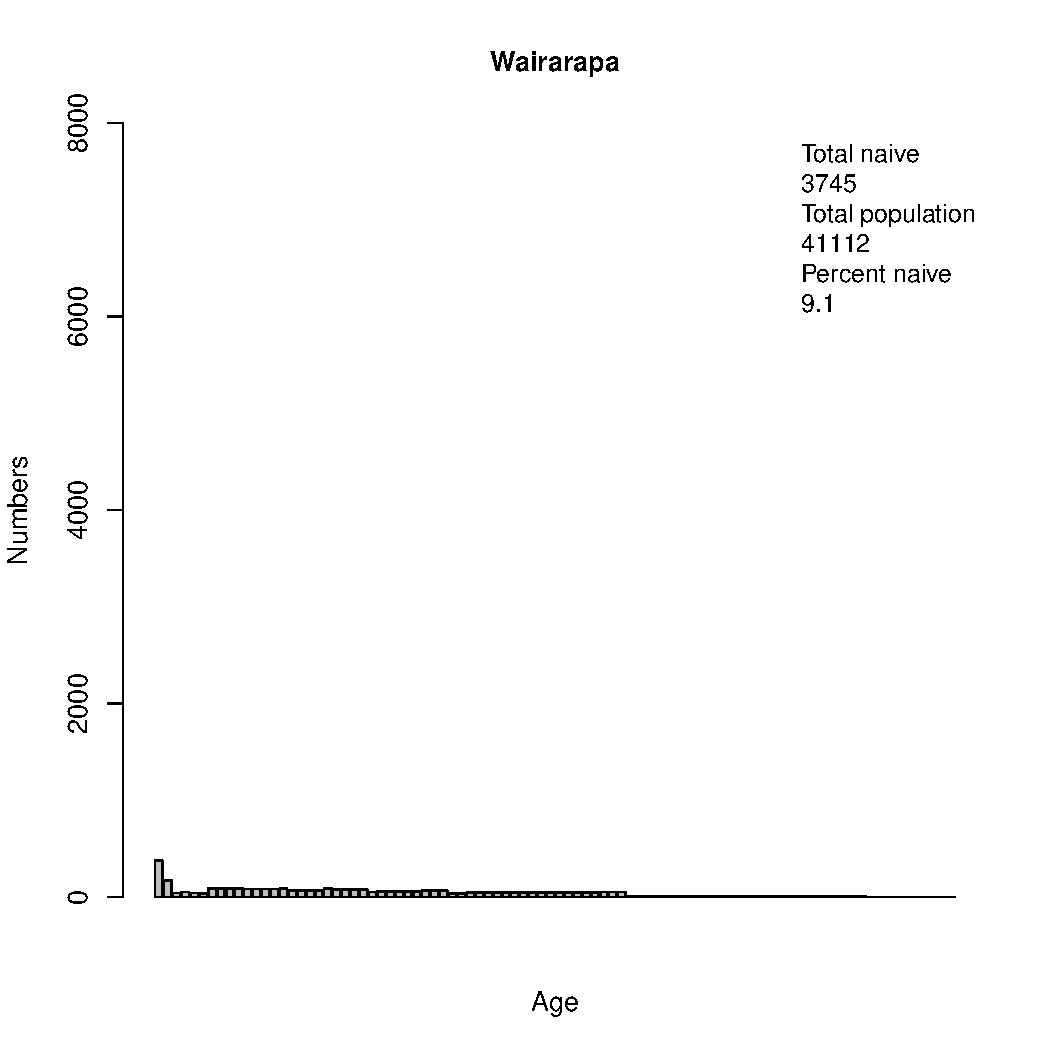
\includegraphics[width=0.6\textwidth]{dhb15.pdf}
     \end{center}
     \caption{Numbers of naive individuals per age class, Wairarapa District Health Board}
     \label{fig:Wairarapa}
\end{figure}

\begin{figure}
     \begin{center}
     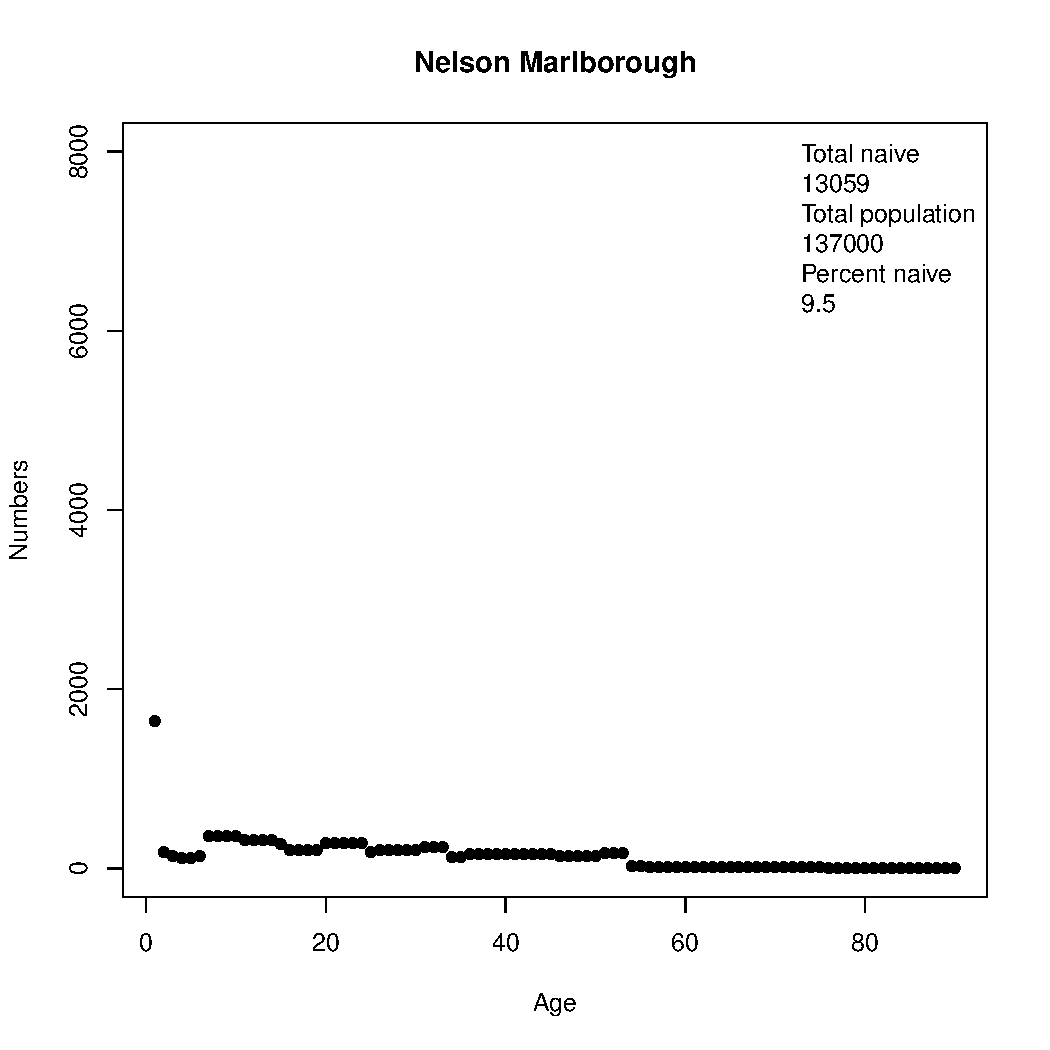
\includegraphics[width=0.6\textwidth]{dhb16.pdf}
     \end{center}
     \caption{Numbers of naive individuals per age class, Nelson Marlborough District Health Board}
     \label{fig:NelsonMarlborough}
\end{figure}

\begin{figure}
     \begin{center}
     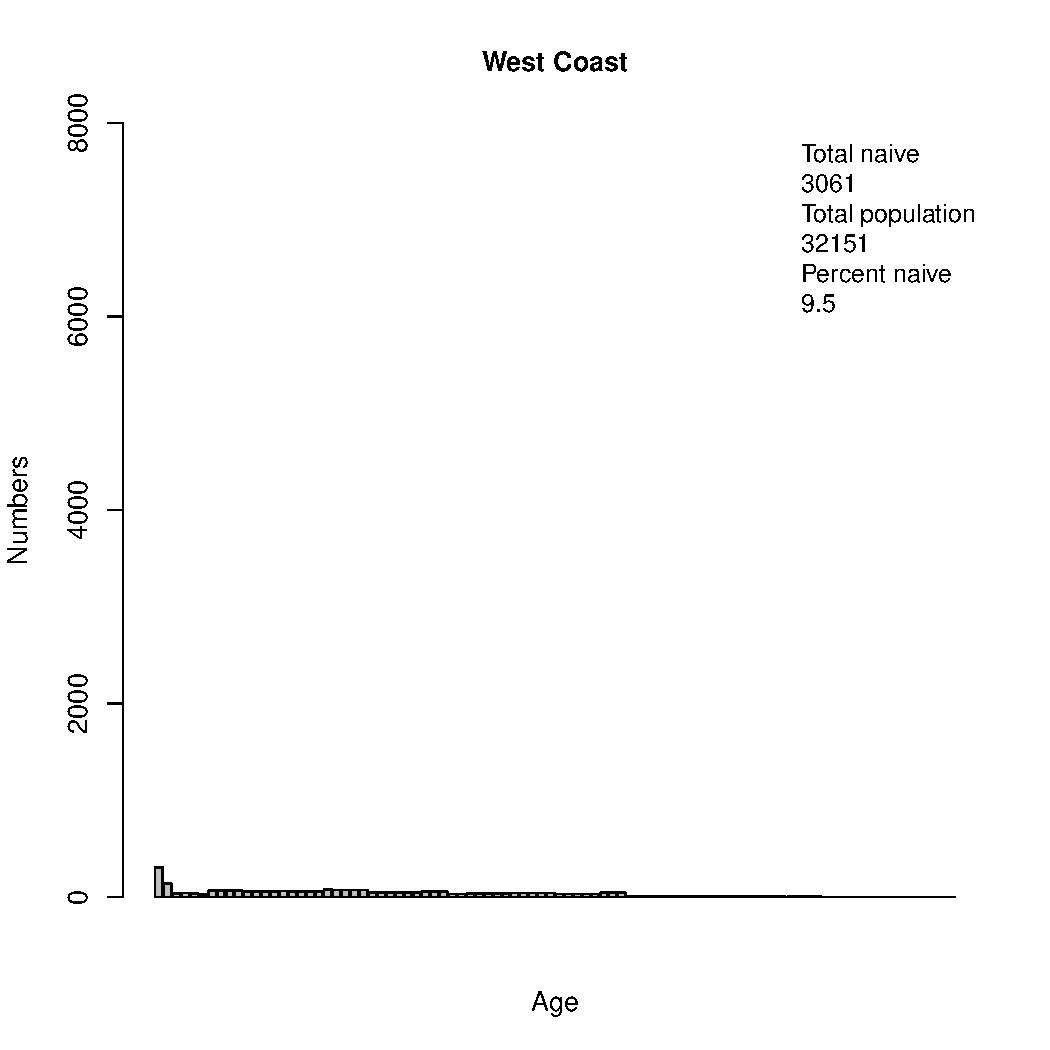
\includegraphics[width=0.6\textwidth]{dhb17.pdf}
     \end{center}
     \caption{Numbers of naive individuals per age class, West Coast District Health Board}
     \label{fig:WestCoast}
\end{figure}

\begin{figure}
     \begin{center}
     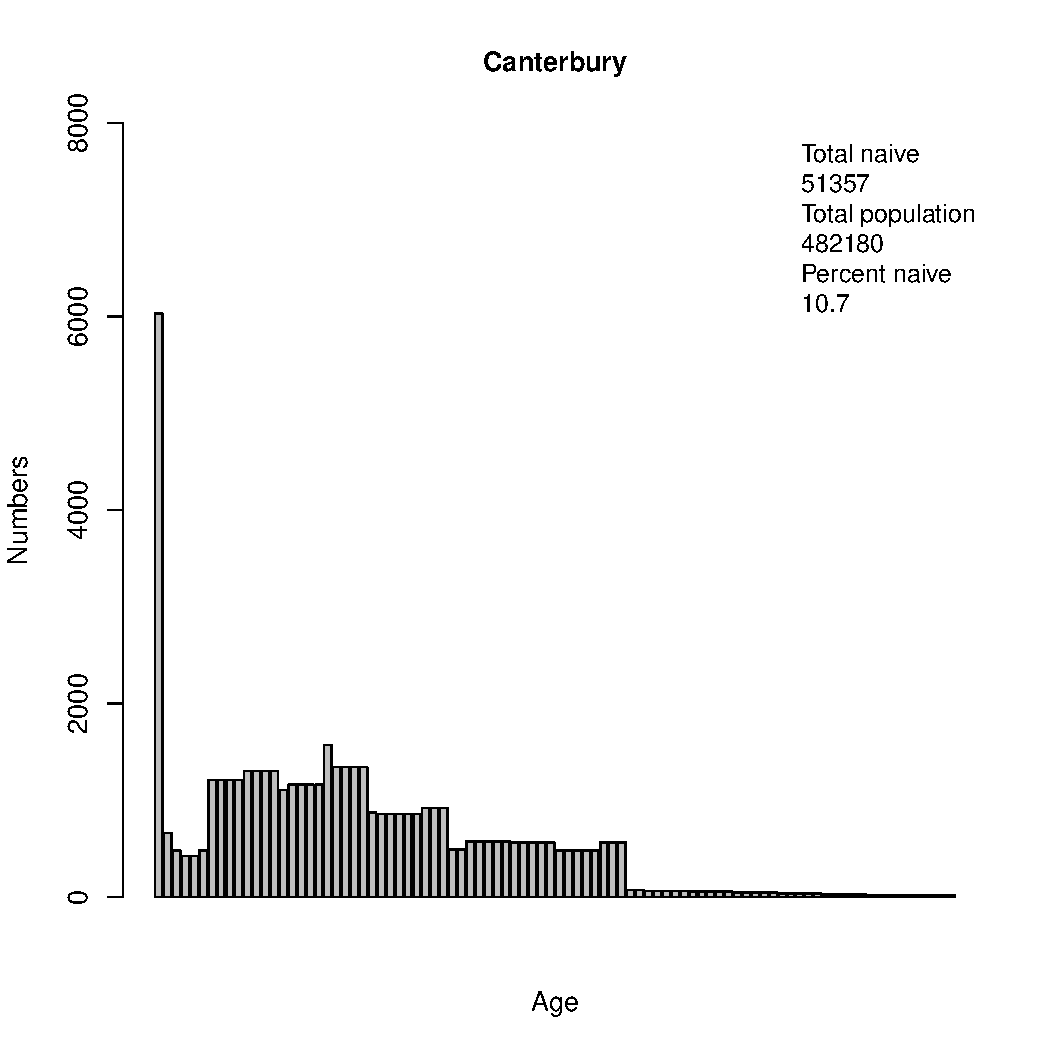
\includegraphics[width=0.6\textwidth]{dhb18.pdf}
     \end{center}
     \caption{Numbers of naive individuals per age class, Canterbury District Health Board}
     \label{fig:Canterbury}
\end{figure}

\begin{figure}
     \begin{center}
     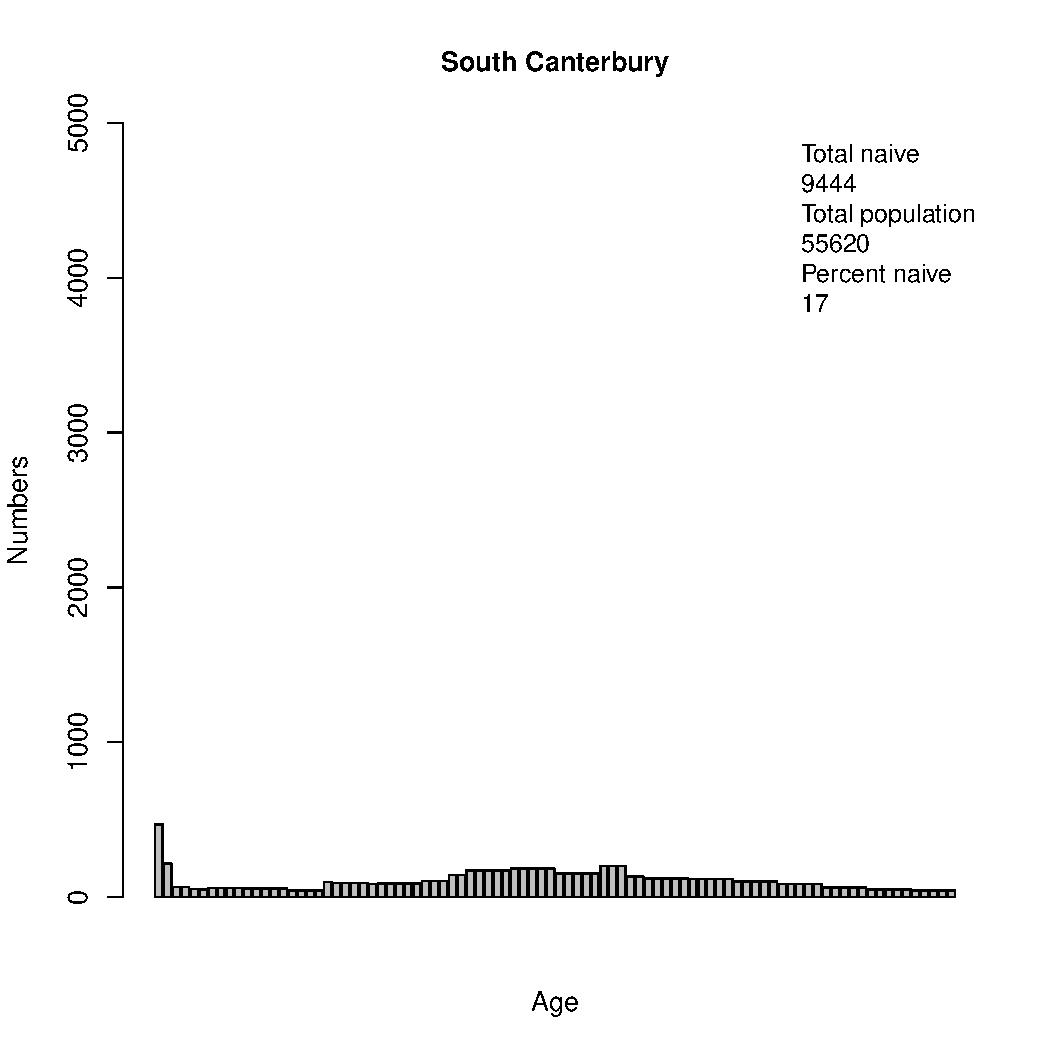
\includegraphics[width=0.6\textwidth]{dhb19.pdf}
     \end{center}
     \caption{Numbers of naive individuals per age class, South Canterbury District Health Board}
     \label{fig:SouthCanterbury}
\end{figure}

\begin{figure}
     \begin{center}
     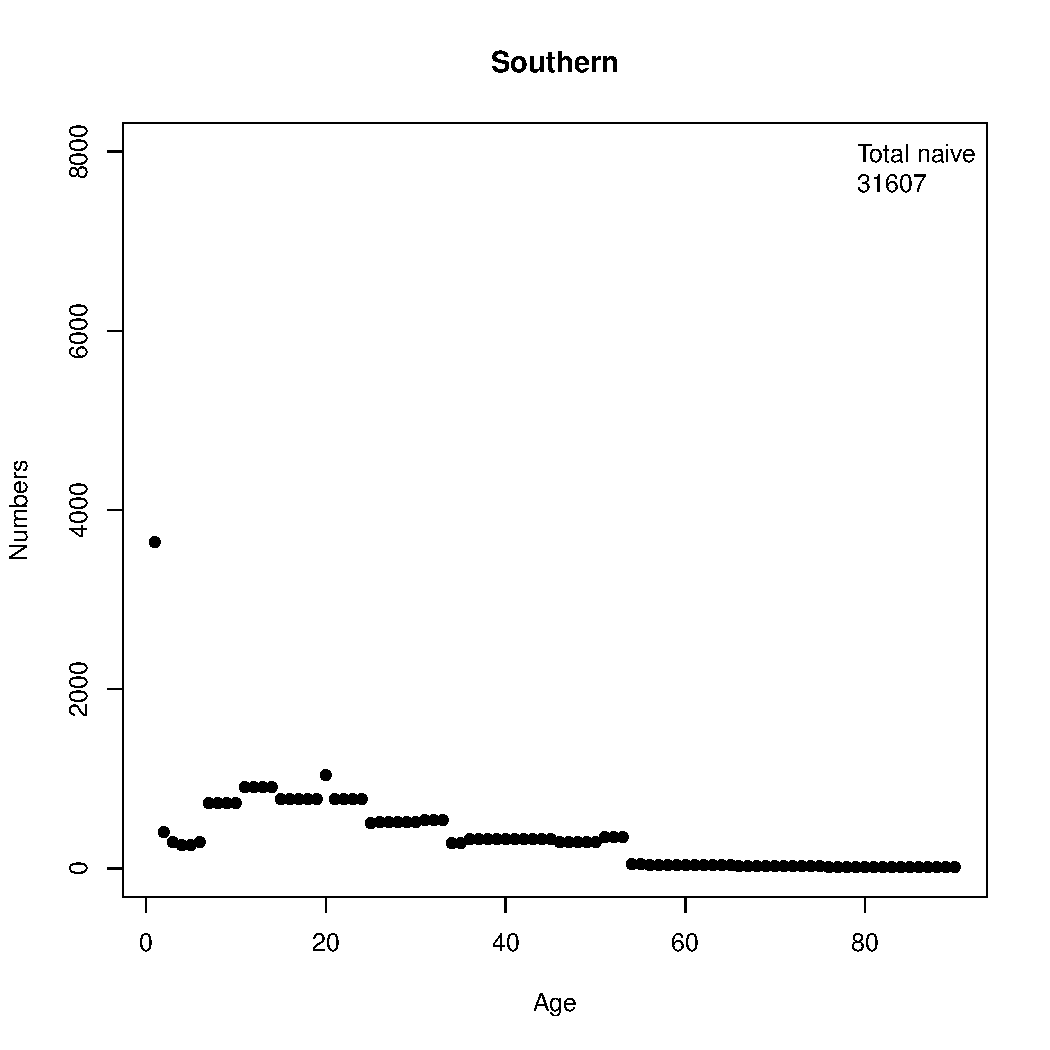
\includegraphics[width=0.6\textwidth]{dhb20.pdf}
     \end{center}
     \caption{Numbers of naive individuals per age class, Southern District Health Board}
     \label{fig:Southern}
\end{figure}

\subsection{Regression analyses results}
\label{sub:regression_results}

The distribution of the cases per category used in the regression analyses are in Figure~\ref{fig:histcasecat}.
\begin{figure}[h!]
\begin{center}
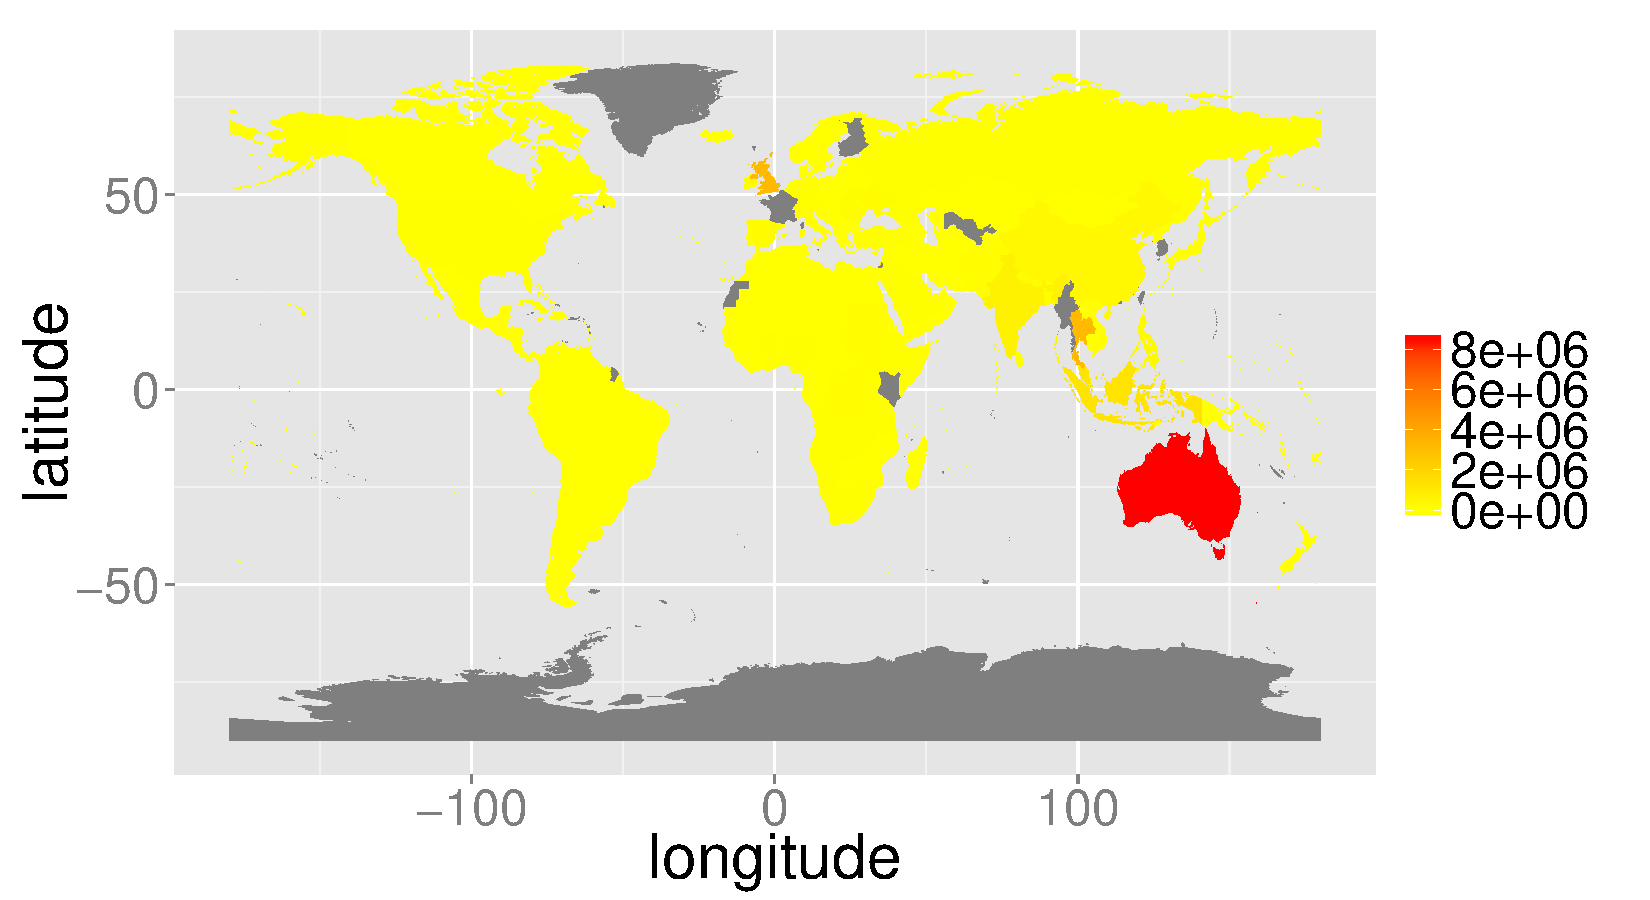
\includegraphics{draftfinalreport-032}
\end{center}
\caption{Distribution of cases per category used in the final regression model}
\label{fig:histcasecat}
\end{figure}

The predicted values from the regression model plotted against the reported cases are shown in Figure~\ref{fig:predict}, and the residuals are shown in Figure~\ref{fig:resid}.
\begin{figure}[h!]
\begin{center}
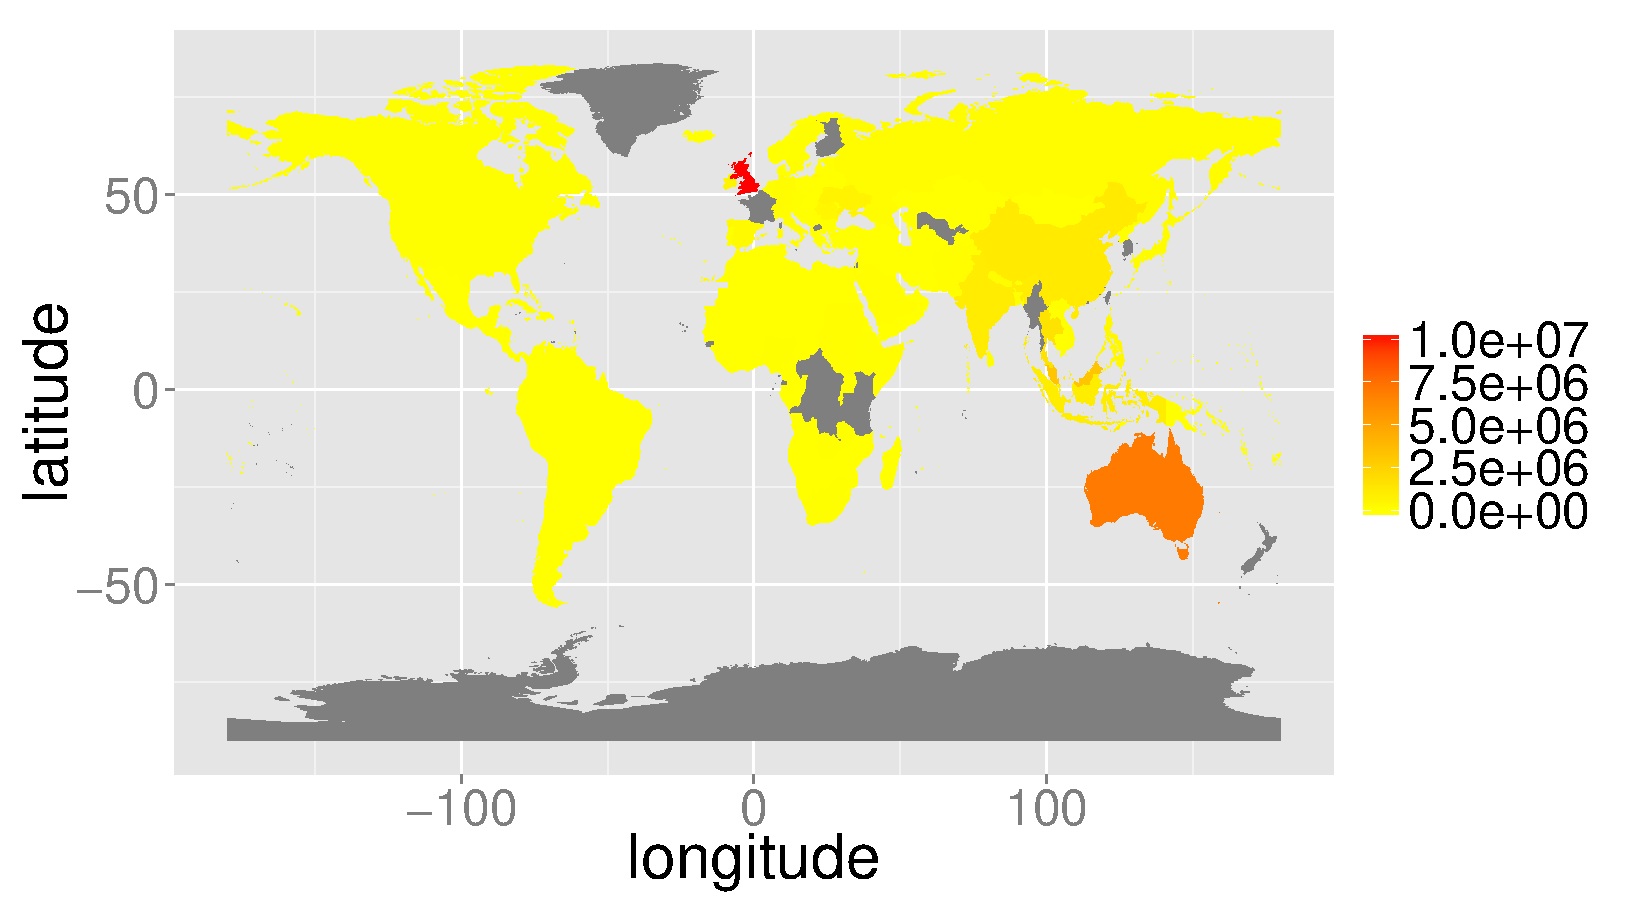
\includegraphics{draftfinalreport-033}
\end{center}
\caption{Regression model (Equation~\ref{eq:reg}) predictions plotted against the cases (Table~\ref{table:percap})}
\label{fig:predict}
\end{figure}


\begin{figure}[h!]
\begin{center}
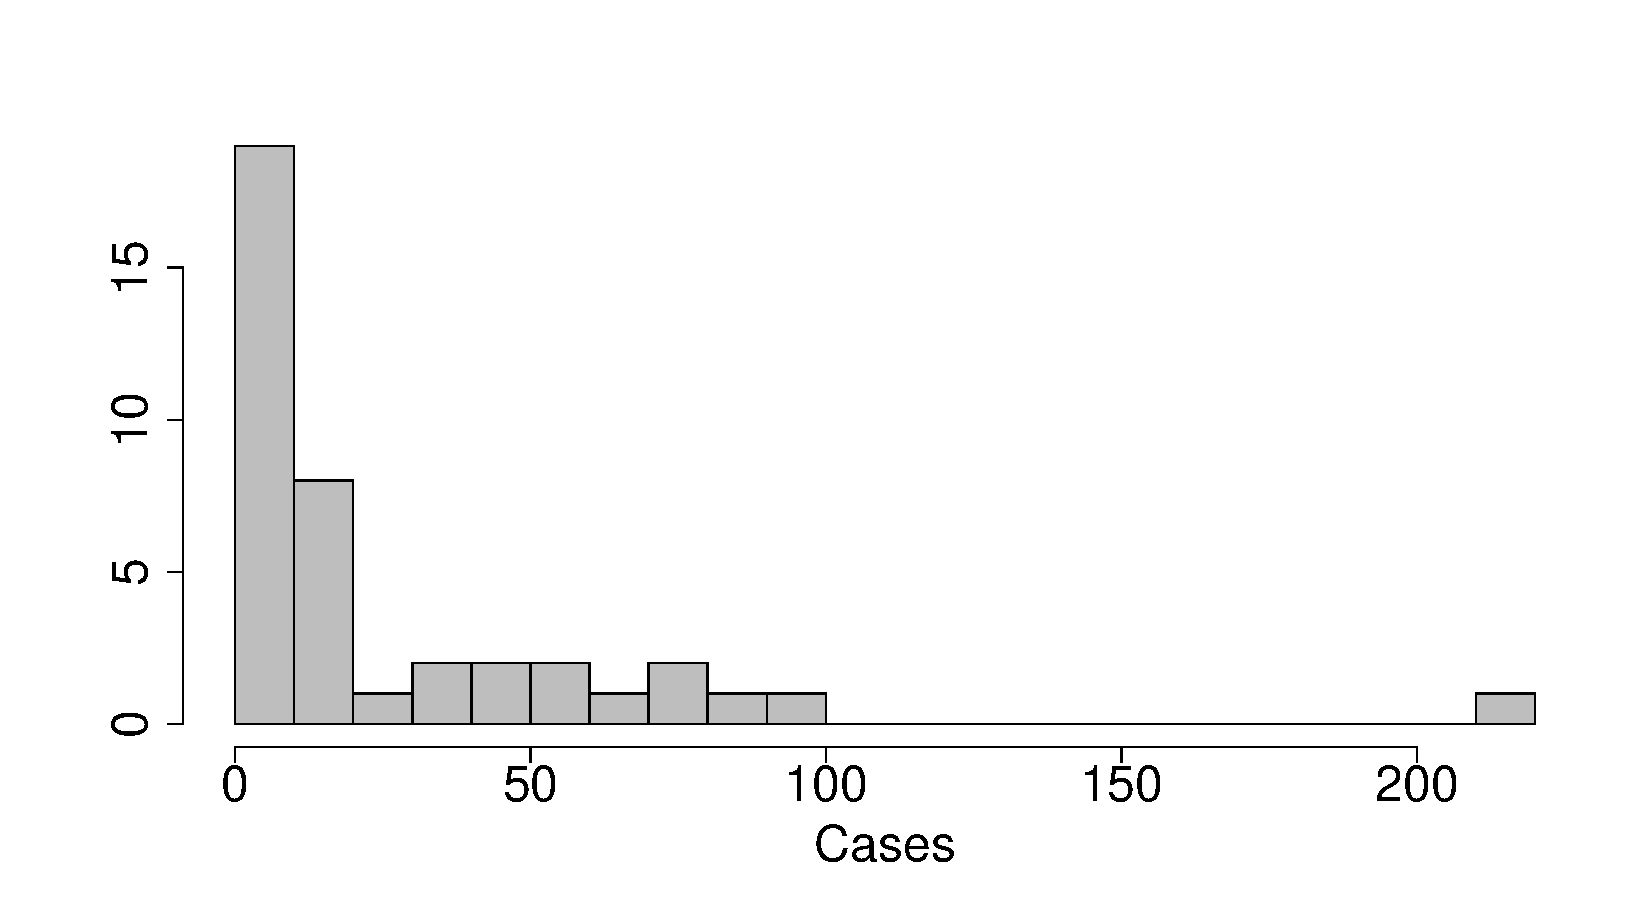
\includegraphics{draftfinalreport-035}
\end{center}
\caption{Histogram of residuals from the regression model (Equation~\ref{eq:reg})}
\label{fig:resid}
\end{figure}
The significance of the different predictor variables can be seen in the ANOVA results:

\begin{Schunk}
\begin{Sinput}
> anova(model3,test="F")
\end{Sinput}
\begin{Soutput}
Analysis of Deviance Table

Model: quasipoisson, link: log

Response: cases

Terms added sequentially (first to last)


              Df Deviance Resid. Df Resid. Dev        F   Pr(>F)    
NULL                             39    1453.62                      
Age            4  1304.20        35     149.43 183.5795 6.73e-15 ***
Ethnicity      3    20.00        32     129.43   3.7529 0.028500 *  
NZDep          1    10.70        31     118.74   6.0236 0.023932 *  
Age:Ethnicity 12    81.91        19      36.83   3.8430 0.004459 ** 
---
Signif. codes:  0 '***' 0.001 '**' 0.01 '*' 0.05 '.' 0.1 ' ' 1
\end{Soutput}
\end{Schunk}

A summary of the regression model (Equation~\ref{eq:reg}) with the individual effects and the statistical support for the estimated coefficients can be seen here:

\begin{Schunk}
\begin{Sinput}
> summary(model3)
\end{Sinput}
\begin{Soutput}
Call:
glm(formula = cases ~ Age + Ethnicity + NZDep + Age:Ethnicity + 
    offset(log(Popn)), family = "quasipoisson", data = tpsub)

Deviance Residuals: 
     Min        1Q    Median        3Q       Max  
-2.76316  -0.52409   0.04736   0.49883   1.92918  

Coefficients:
                          Estimate Std. Error t value Pr(>|t|)    
(Intercept)               -6.46738    0.11483 -56.324  < 2e-16 ***
Age3-5                    -0.91290    0.20539  -4.445 0.000278 ***
Age6-17                   -0.76175    0.13427  -5.673 1.81e-05 ***
Age18-24                  -1.50501    0.19366  -7.772 2.57e-07 ***
Age25+                    -2.95073    0.16079 -18.352 1.51e-13 ***
EthnicityAsian             0.05304    0.32498   0.163 0.872072    
EthnicityMaori             0.21245    0.19935   1.066 0.299919    
EthnicityPacific           1.16032    0.20429   5.680 1.78e-05 ***
NZDep6-10                 -0.21192    0.08548  -2.479 0.022713 *  
Age3-5:EthnicityAsian     -2.03154    1.38265  -1.469 0.158112    
Age6-17:EthnicityAsian    -1.00742    0.47171  -2.136 0.045940 *  
Age18-24:EthnicityAsian   -0.83115    0.59409  -1.399 0.177917    
Age25+:EthnicityAsian      0.42108    0.44334   0.950 0.354143    
Age3-5:EthnicityMaori     -0.38639    0.40959  -0.943 0.357344    
Age6-17:EthnicityMaori    -0.08552    0.24685  -0.346 0.732812    
Age18-24:EthnicityMaori   -0.58278    0.44835  -1.300 0.209209    
Age25+:EthnicityMaori     -1.04821    0.52418  -2.000 0.060036 .  
Age3-5:EthnicityPacific   -2.13163    0.81388  -2.619 0.016882 *  
Age6-17:EthnicityPacific  -1.45411    0.33466  -4.345 0.000349 ***
Age18-24:EthnicityPacific -0.98266    0.51289  -1.916 0.070546 .  
Age25+:EthnicityPacific   -0.61270    0.43665  -1.403 0.176692    
---
Signif. codes:  0 '***' 0.001 '**' 0.01 '*' 0.05 '.' 0.1 ' ' 1

(Dispersion parameter for quasipoisson family taken to be 1.776063)

    Null deviance: 1453.62  on 39  degrees of freedom
Residual deviance:   36.83  on 19  degrees of freedom
AIC: NA

Number of Fisher Scoring iterations: 5
\end{Soutput}
\end{Schunk}

Apart from over-representation of some MLA categories discussed above and not included here, the results of the regression model suggest that age is a strong predictor of being a measles case. Indeed, all age categories are significantly less likely to be measles cases compared to 0-2 year olds, and the likelihood decreases with age (Figure~\ref{fig:ageinyears}).

People of Pacific origin are also over-represented ($\beta$ = 1.16, standard error (SE) = 0.2, p--value < 0.0001), NZDep levels 6-10 under-represented ($\beta$ = -0.21, SE = 0.085, p--value = 0.02), and there are some other age:ethnicity classes that are significantly less represented in the data compared to Europeans in those ages classes, particularly in the 6--17 age classes. In later outbreaks (since 2007) there has been a shift in the distribution of ages infected. The very young are still most likely to be infected, but of school aged children older teenagers are more likely to be represented then the under tens (Figure~\ref{fig:ageinyears}). This pattern suggests that improving vaccination coverage in the young is reducing the burden of measles in those age categories. Interestingly the regression results suggest risk of measles cases in the 6--17 year age category was greater for Europeans and Maori.


\subsection{Risk analysis discussion}

The regression analyses suggest that age is a particularly strong risk factor for measles. This comes as no surpise to epidemiologists or health care providers. However, our analyses also highlight other groups that are at greater risk of measles. In particular, Pacific people are at greater risk, as are the more wealthy (NZDep 1--5), and European and Maori 6--17 year old children compared to Asian and Pacific ethnicity children of the same age. Interpretation of these results must still be viewed with some caution, however, as there is very likely a spatial effect that might not be accounted for in these analyses. Additional data we have been provided by the Ministry of Health but are yet to incorporate in our risk analyses are finer scale (domicile level) immunisation coverage data from the National Immunisation Register (NIR). A key issue with incorporating spatial immunisation data has been the denominator data, and how to deal with people of greater age than those recorded in the NIR. These analyses are possible future directions for this work. The results of these regression analyses are also discussed in the benefit--cost section below (Section~\ref{sub:cost_benefit})

\subsection{Risk analysis summary}
\begin{itemize}
\item There is a continued, and perhaps increasing, risk of measles importation due to travel and endemic measles elsewhere in the world.
\item There may be seasonal changes in risk of measles importation, though further analyses are needed.
\item Risk of measles infection decreases significantly with age
\item Pacific people are statistically more at risk of measles infection
\item There is some statistical support for those living in better socio-economic situations being at greater risk of measles
\item There is some statistical support for Pacific and Asian children in the 6--17 year age categories being at lower risk than European or Maori children
\end{itemize}

\subsection{Future risk analyses}
We received the raw EpiSurv measles case data from The Institute of Environmental Science and Research Ltd (ESR) on 27 June 2014. Initial analyses of those data (not shown) suggest that we require denominator data to perform multivariate analyses to avoid confounding results due to a lack of independence among risk factors. Specifically for the multivariate analyses we wish to perform that detect interactions we require $\textsf{Age} \times \textsf{Prioritised Ethnicity} \times \textsf{NZDep}$ data for New Zealand to test whether interactions among case covariates provide additional information on risk over the univariate analyses performed in the report reviewed above. These $\textsf{Age} \times \textsf{Prioritised Ethnicity} \times \textsf{NZDep}$ data only became available to us on 3 July 2014, provided by the University of Otago.

The following analyses are in progress, for inclusion in later reports:
\begin{itemize}
\item Multivariate regression analyses to assess interactions between risk factors that may confound the univariate analyses.
\item Update of the importation risk analyses using a broader range of years, including modelling the trend in importations.
\end{itemize}
Additional data we believe would enable us and the Ministry to better understand measles risk is fine scale (lower than District Health Board (DHB)) immunisation coverage data. We understand the National Immunisation Register (NIR) allows tracking of the vaccination status of children and this is very useful, but inclusion of these data at lower (e.g. meshblock, census area unit) level would allow better understanding of risk of measles infection and resource allocation because they may allow targeted immunisation programmes. Thus the data gap that we have that will hinder us providing fine scale risk maps is:
\begin{itemize}
\item Meshblock (or census area unit) level immunisation coverage data to allow targeted immunisation and understanding of risk at a fine scale level.
\end {itemize}
An additional data set that would enable us to develop the understanding of measles importation risk is:
\begin {itemize}
\item The number of New Zealanders arriving from abroad each year, the countries to which they travelled, and length of travel.
\end{itemize}


\section{Modelling measles epidemics}
\label{sec:epidemic_modelling}

A previously-published model of the dynamics of measles infections in New Zealand has been used to evaluate the vaccination strategy in New Zealand of MMR1 at 15 months and MMR2 before 5 years \citep{roberts0,roberts4,tobias98}. The results show that achieving coverage of greater than 90\% at both vaccination opportunities is necessary if future epidemics of measles are to be prevented.

The original mathematical model for the dynamics of measles in New Zealand prepared in 1996 \citep{tobias98} successfully predicted the 1997 epidemic, which was curtailed by a mass vaccination campaign \citep{mansoor98,roberts0}. Subsequent extension of this work in 1998 showed that the then current schedule of MMR1 at 15 months and MMR2 at 11 years was insufficient to prevent further epidemics. The model developed by \citep{roberts0} supported the change in the immunisation schedule that took effect in January 2001, at which time MMR2 was changed from delivery at 11 years to delivery before the age of five. The schedule was changed in 2000 with MMR2 now being administered before 5 years \citep{anon2a} and later analyses suggested high levels of vaccination coverage (but less than 95\%) could eliminate measles, but emphasised that it is necessary to maintaining high coverage rates in order to prevent future epidemics \citep{roberts4}.

These results were comparable to others, for example: \citep{babad95} suggested two-dose schedule for England and Wales, with the second vaccination given at age four; and \citep{gay98} recommended a second vaccination at either 18 months or five years, to complement the first vaccination at 12 months in Canada. In addition, \citep{agur93} found that vaccinating 85\% of susceptible children aged one to seven years at five-yearly intervals would prevent epidemics in Israel. All agree that two vaccinations at no less than five years apart are necessary to prevent measles epidemics. \citep{wallinga1} took existing policies in eight European countries and estimated the coverage rates required to reduce $R_v$ below one. They found that results depended on the age at delivery, but no strategy succeeded if coverage rates were below approximately 87\%.

Numerous models for measles vaccination strategies for various regions \citep{agur93, babad95, edmunds0, gay98, wallinga1} based on sets of nonlinear differential equation (ODE) models have reached similar conclusions. The differences in the models have been in the details of the representation of the infectious period, and in the ways in which the age and contact structures of the population have been specified. While analyses suggest that 85\% coverage at MMR1 and MMR2 could be sufficient to prevent future measles epidemics, \citep{glass4} in the Netherlands showed that high overall levels of measles vaccination can obscure pockets of poor coverage, resulting in localised regions with increased risk of infection and effective immunisation is difficult to evaluate. 

The quantity that determines whether an epidemic will occur is the basic reproduction number of the infection, $R_0$. This is defined as the expected number of secondary infections that would arise from a single primary infection introduced into a fully susceptible population \citep{anderson91, diekmann0}. If $R_0 > 1$ an epidemic will occur following an introduction of infection. The best estimate for measles in New Zealand was $R_0$ = 12.8 \citep{roberts4}. The basic reproduction number of the infection under vaccination, $R_v$, is the expected number of secondary infections that would arise from a single primary infection introduced into a vaccinated population at equilibrium and is a robust indicator of the performance of a vaccination schedule. If $R_v < 1$ epidemics are prevented. The case reproduction number of the infection at time $t$, $R_t$, is the expected number of secondary infections that arise from a single infection at a particular time and depends on the number in the population who are susceptible.

\subsection{Modelling methods}

To understand the level of immunity in the population, the transmission dynamics of measles in the partially immune population and how likely an outbreak was of becoming endemic, we estimated $R_v$ from all the outbreaks in New Zealand since 2009. To do this we estimated $R_t$, following an adaptation of the methods in \citep{obidia12,wallinga4}. We were required to compute the generation time for measles to do so. The generation time is the average time an index case infects others after becoming infected. We used a lognormal distribution with mean 12.0 and standard deviation (s.d.) 3.5 from \citep{klinkenberg11}. We then estimated $R_t$ from the incidence data for each outbreak, defining outbreaks in the dataset given their temporal and geographic correlations (Figure~\ref{fig:dhbcases}). The outbreaks we used in our analyses are shown in Figure~\ref{fig:outbreaks}.


\begin{figure}
     \centering
     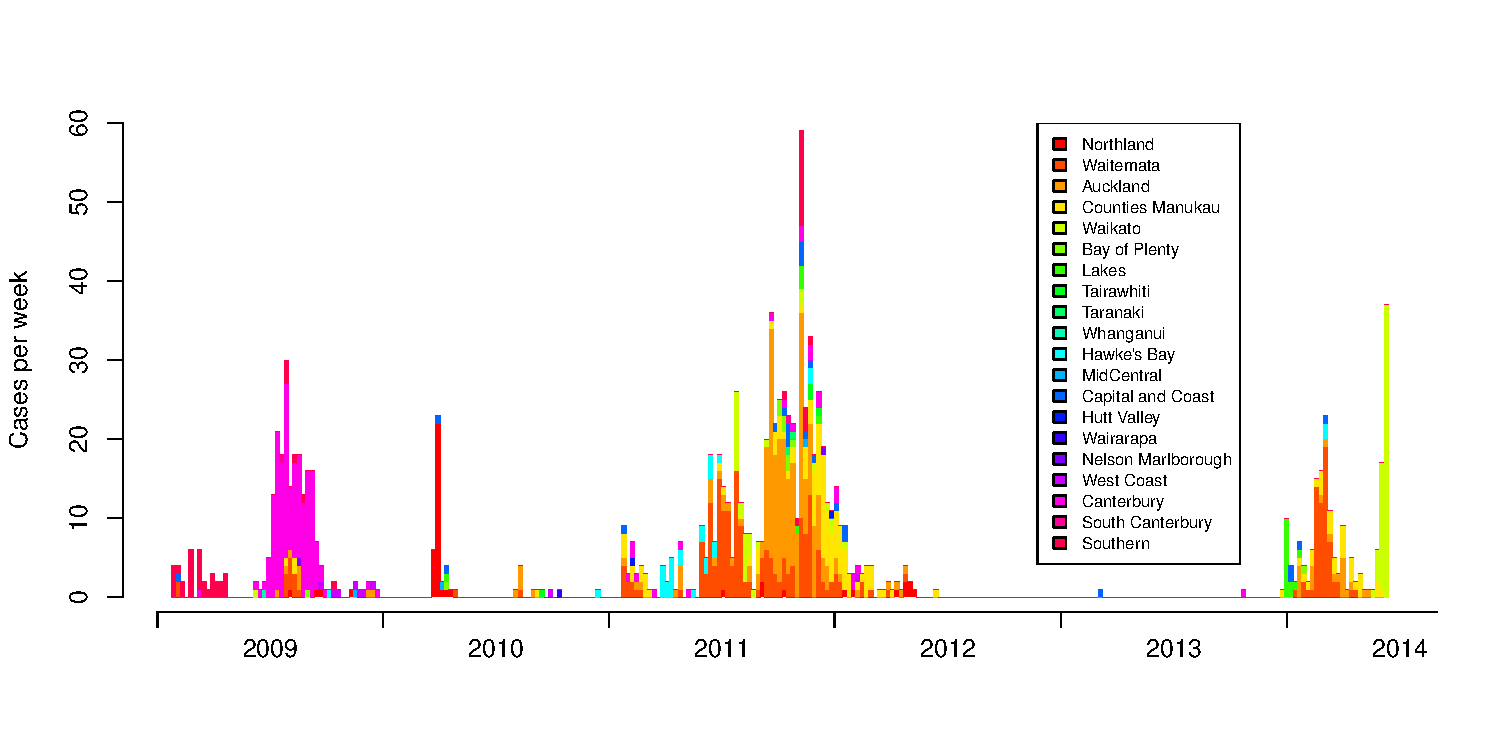
\includegraphics[width=0.9\textwidth]{cases_by_dhb_2009_2014.pdf}
     \caption{Measles cases by district health board (DHB) from 2009 to 2014}
     \label{fig:dhbcases}
\end{figure}

\begin{figure}
     \centering
     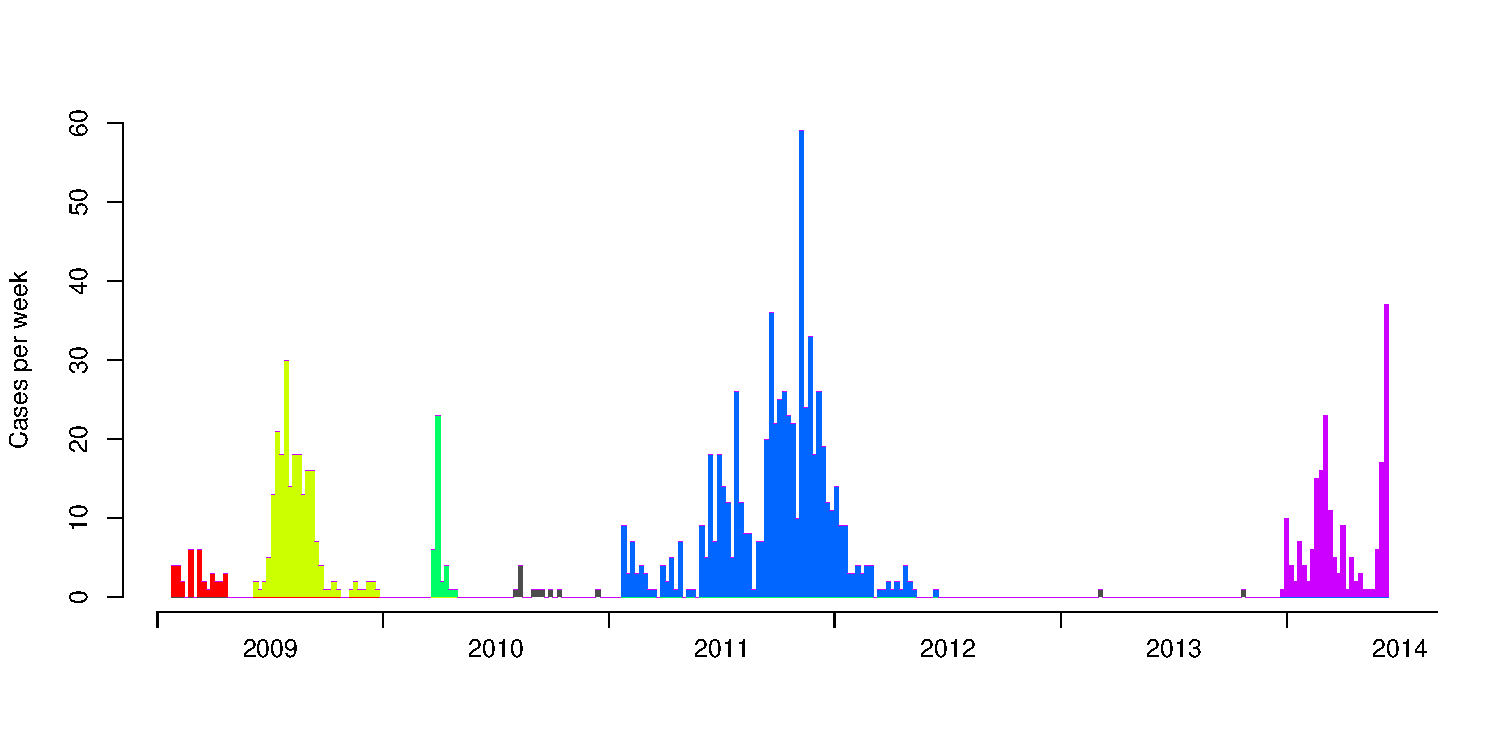
\includegraphics[width=0.9\textwidth]{outbreaks_for_R0.pdf}
     \caption{Measles data classified as outbreaks for reproductive number of the infection ($R_v$) estimation}
     \label{fig:outbreaks}
\end{figure}

\begin{figure}
     \centering
     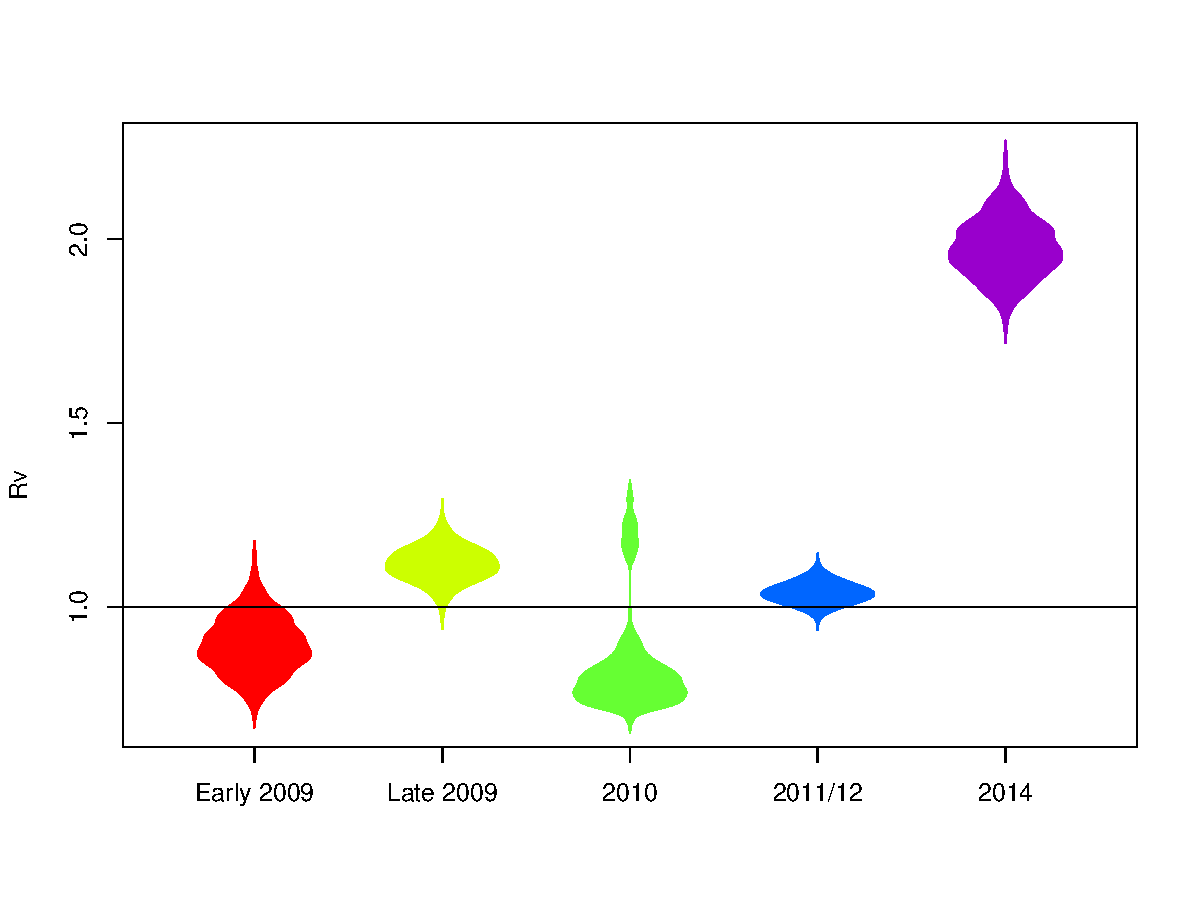
\includegraphics[width=0.9\textwidth]{averageR0.pdf}
     \caption{Estimates of $R_v$ (Average $R_0$) for the outbreaks each year, as classified by outbreaks in Figure~\ref{fig:outbreaks}}
     \label{fig:r0}
\end{figure}

To estimate the proportion of the population requiring vaccination utilising our estimates of $R_v$, we make several simplifying assumptions regarding the relationship between the proportion requiring vaccination, $p_c$, and $R_0$. Specifically, we use the simple relationship:

\begin{equation} \label{eq:pc}
p_c = 1-(1/R_0)
  \end{equation}
To account for the different outbreak sizes we weighted our $R_v$ estimates by outbreak size and used 1.96 standard deviations of the mean of our $R_v$ estimates, to generate 95\% confidence limits from 2009--2014 outbreaks or the 2013--2014 outbreak for our modelling scenarios below.

We then assume that the measles epidemics are occurring in a naive population that is the size of the naive and currently susceptible population remaining in New Zealand and thus $R_0$ is equivalent to $R_v$. We estimated the susceptible population in New Zealand from the national level vaccination coverage data provided by the Ministry of Health for this work (approximately 11\%, Figure~\ref{fig:naive}). Thus, the $p_c$ applies to the naive population in New Zealand and these are the additional vaccinations required to reduce $R_v$ to one in the overall New Zealand population.


\begin{figure}[ht!]
\begin{center}
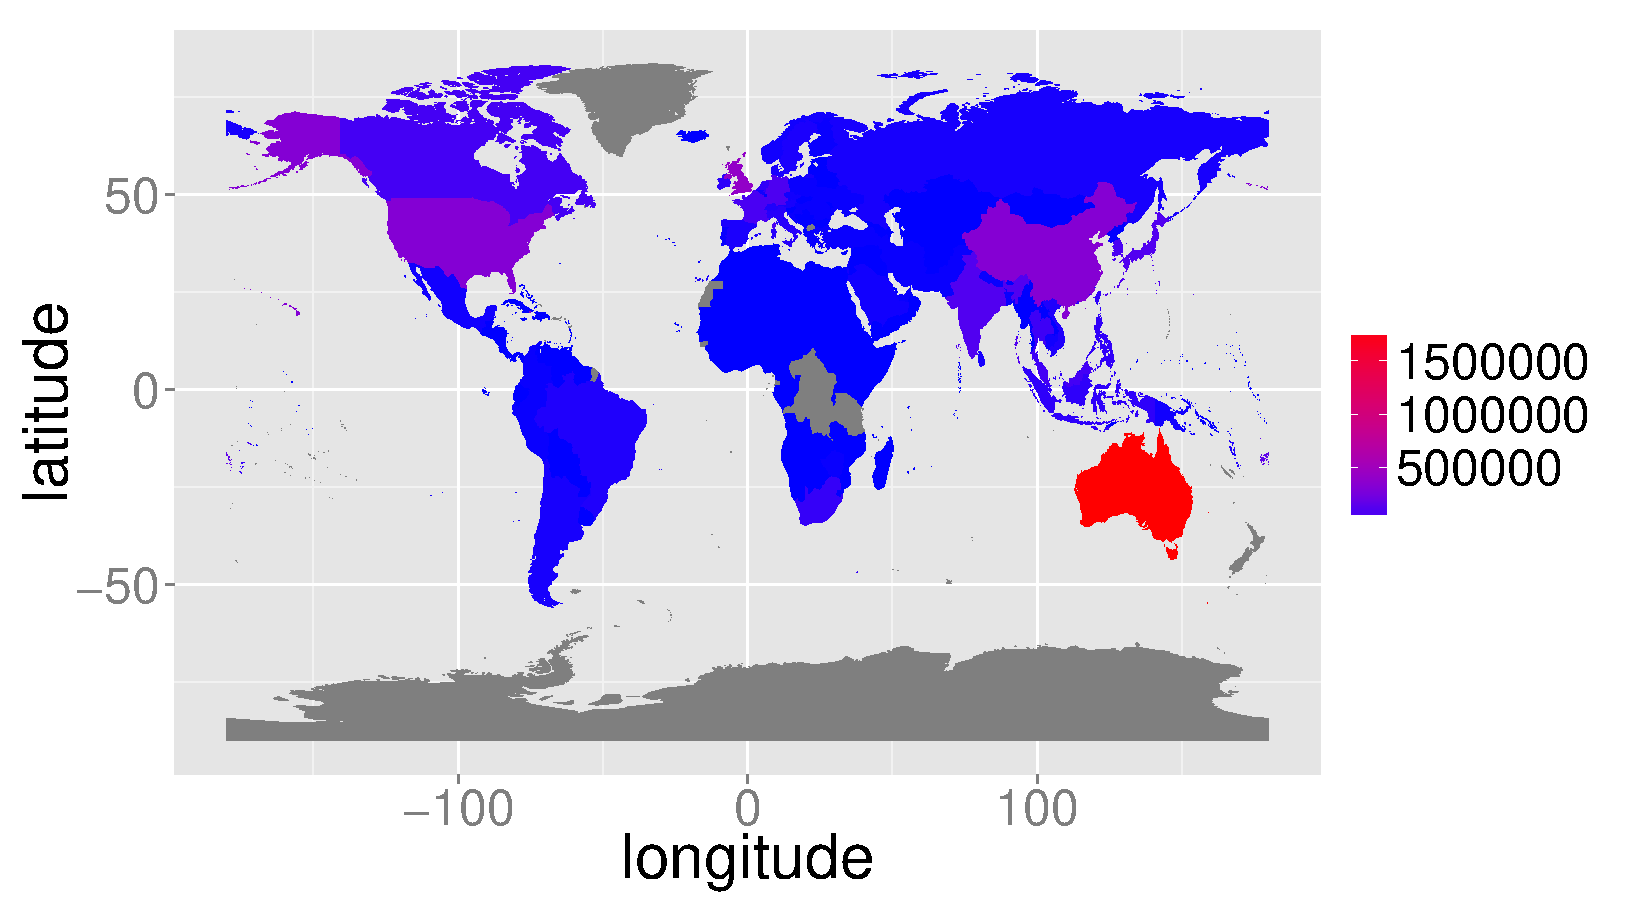
\includegraphics{draftfinalreport-039}
\end{center}
\caption{New Zealand population by age and estimated numbers of naive people in each age class}
\label{fig:naive}
\end{figure}

We then used the proportions of the population that were estimated to require vaccination ($p_c$, Equation~\ref{eq:pc}), and the proportions of the naive population per age case from Figure~\ref{fig:naive} to provide different scenarios to achieve those goals. These are explored and discussed in relation to the risk analyses (Section~\ref{sub:regression_results}) in the benefit--cost analyses section below (Section~\ref{sub:cost_benefit}).

Finally, we used the same model structure and generation times to estimate the epidemic sizes once vaccination catch up protocols had been implemented assuming $R_v$ < 1 and the population of susceptible people in New Zealand was now reduced by the numbers vaccinated. Because the model is stochastic, we ran 1000 simulations and report the mean values, though the distribution of these is shown in the benefit--cost section (Section~\ref{sub:cost_benefit}).

\section{Mick Introduction}

The well-known equation for the final size of an epidemic in a homogeneously mixing susceptible population is \citep{diekmann13}
$$\log\left(1-\Pe\right)+\Ro\Pe=0$$
where $\Ro$ is the basic reproduction number and $\Pe$ is the proportion of the population infected over the course of the outbreak.
If a proportion $x_0$ of the population is susceptible following vaccination, then the  reproduction number under vaccination is $\Rr_V=x_0\Ro$, and the final size equation becomes
$$\log\left(1-\frac{\Pe}{x_0}\right)+\Ro\Pe=0$$
Hence the relationship between the proportion initially susceptible and the proportion infected in an epidemic is
$$x_0=\frac{\Pe}{1-e^{-\Ro\Pe}}$$
In order to prevent future epidemics, it is necessary that $\Rr_V<1$. Hence, the proportion of the population that must be vaccinated to prevent future outbreaks is $x_0-1/\Ro$.

These formulae were applied at a District Health Board (DHB) level, assuming no mixing between DHBs.


\begin{figure}
     \centering
     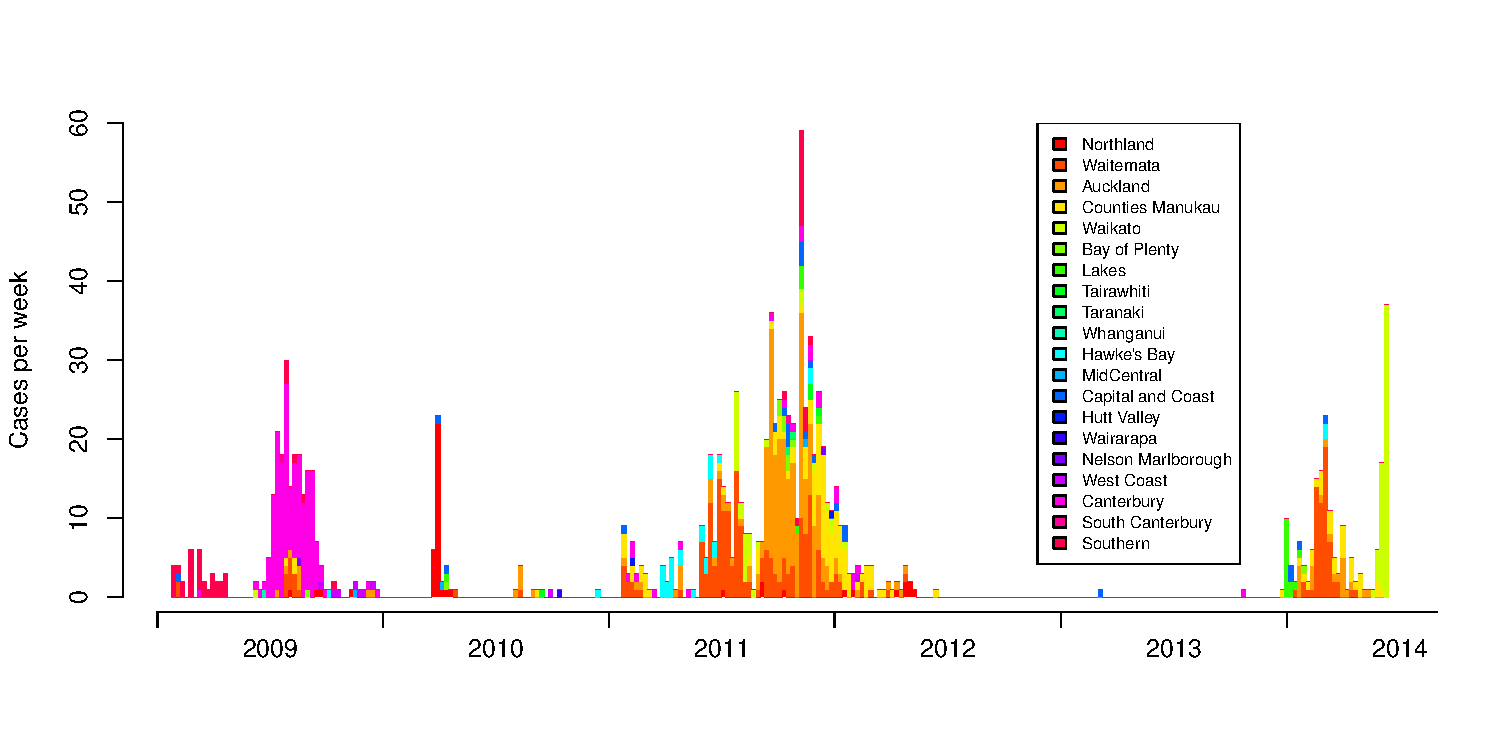
\includegraphics[width=0.8\textwidth]{cases_by_dhb_2009_2014.pdf}
     \caption{Measles cases by district health board (DHB) from 2009 to 2014}
     \label{fig:dhbcases}
\end{figure}

\begin{figure}
     \centering
     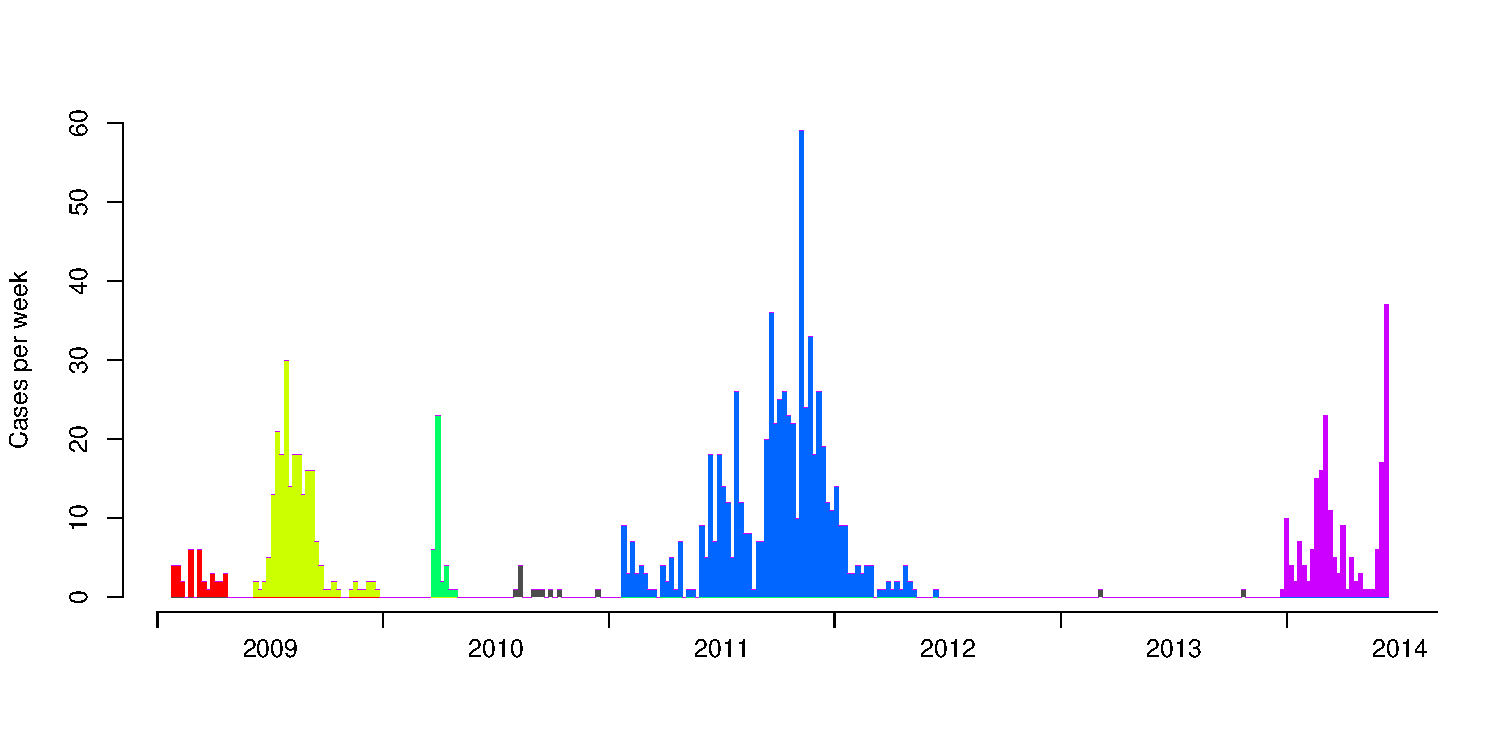
\includegraphics[width=0.8\textwidth]{outbreaks_for_R0.pdf}
     \caption{Measles data classified as outbreaks for reproductive number of the infection ($R_v$) estimation}
     \label{fig:outbreaks}
\end{figure}

\begin{figure}
     \centering
     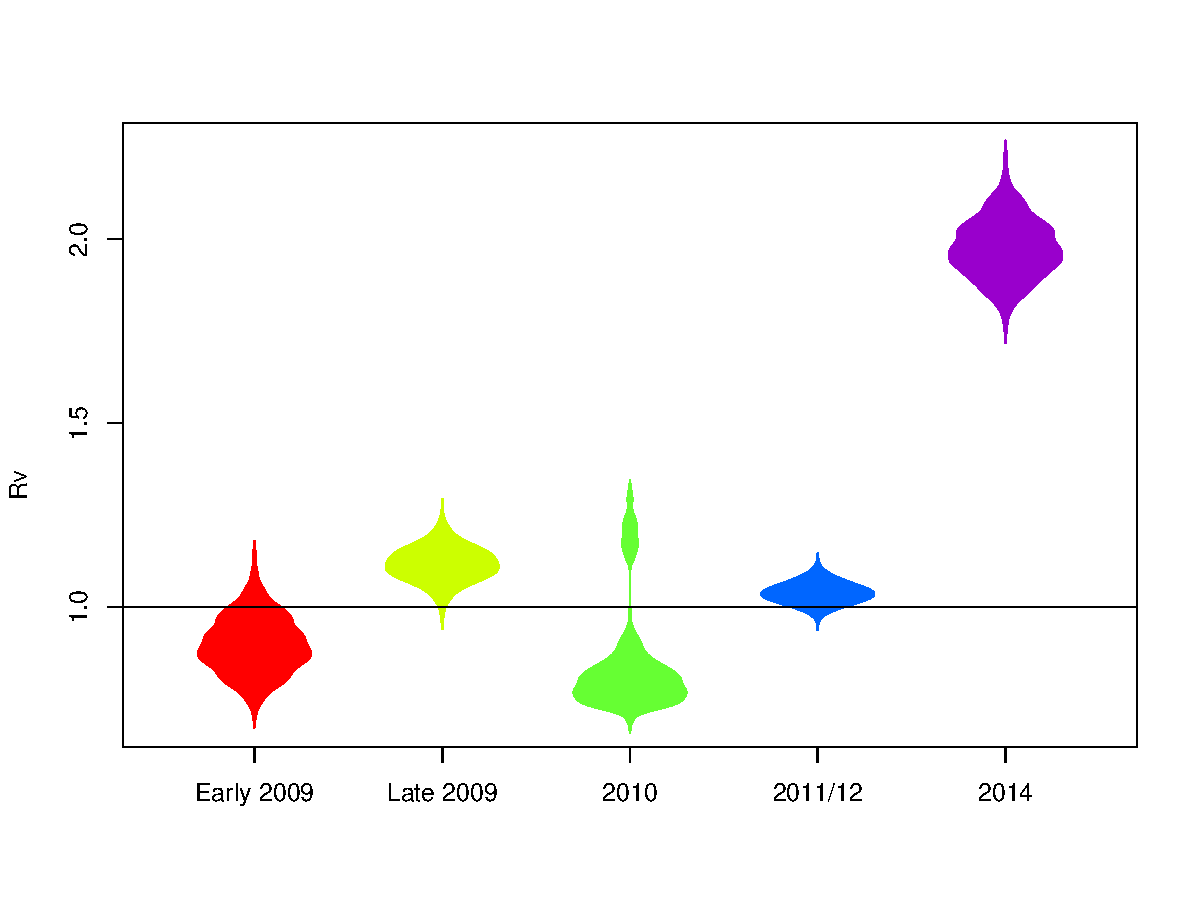
\includegraphics[width=0.8\textwidth]{averageR0.pdf}
     \caption{Estimates of $R_v$ ($R_0$) for the outbreaks each year, as classified in Figure~\ref{fig:outbreaks} (page~\pageref{fig:outbreaks})}
     \label{fig:r0}
\end{figure}

\subsection{Modelling results and discussion}

The estimated $R_v$ for each outbreak is shown in Figure~\ref{fig:r0}. The probability density of the $R_v$ estimates for each outbreak all include one. Of particular note is the ongoing outbreak, which has an $R_v$ well above one and thus we may expect this outbreak to persist if conditions remain the same. An important caveat to this outbreak analysis is that because this 2013--2014 outbreak is an ongoing outbreak, and not in decline, $R_0$ is necessarily over one, and so the comparison with others must be cautious.

These analyses also imply that the regular (approximately yearly) importation of measles is an ongoing process. Given the risk of importation of measles as highlighted in section~\ref{sub:risk_analyses} is likely to continue, these analyses suggest substantial efforts are required to maintain the level of immunisation to high enough levels that measles does not become endemic. The measles outbreak in 2011--2012 had an $R_v$ of just greater than one, and yet it persisted for over 12 months. This implies that the current outbreak may persist within the population for a substantial period, given it's $R_v$ is approximately twice that of the 2011-2012 outbreak. A caveat to this and other $R_v$ estimates is that the 2013--2014 outbreak may include some sporadic cases and thus the true basic reproductive numbers may be lower than estimated. However, sub-clinical and underreporting may lower the estimate. The relative contributions of both to our estimates are currently unknown.

The estimated $R_v$ for each outbreak is shown in Figure~\ref{fig:r0} and in the previous interim report. The probability density of the $R_v$ estimates for each outbreak all include one, except for the ongoing 2013--2014 outbreak, which has an $R_v$ well above one. As discussed in the previous interim report, the important caveat to this outbreak analysis is that because this 2013--2014 outbreak is an ongoing outbreak, and not in decline, $R_v$ is necessarily over one, and so the comparison with others must be cautious. However, the results of these differences are presented and discussed in the benefit--cost analysis section (Section~\ref{sub:cost_benefit}). The 95\% confidence intervals for our analyses suggest the $R_v$ for the 2009--2014 outbreaks is 0.92--1.19, and for the current outbreak 1.82--2.13.

The regularity of these outbreaks also imply that the regular (approximately yearly) importation of measles is an ongoing process. Given the risk of importation of measles as highlighted in section~\ref{sub:risk_analyses} and our previous report is likely to continue, we explore the effects of this in the benefit--cost section (Section~\ref{sub:cost_benefit}).

The measles outbreak in 2011--2012 had an $R_v$ of just greater than one, and yet it persisted for over 12 months. This implies that the current outbreak may persist within the population for a substantial period, given it's $R_v$ is approximately twice that of the 2011-2012 outbreak. A caveat to this and other $R_v$ estimates is that the 2013--2014 outbreak may include some sporadic cases and thus the true basic reproductive numbers may be lower than estimated. However, sub-clinical and underreporting may lower the estimate. The relative contributions of both to our estimates are currently unknown.

To use the results from our modelling exercise to help inform the appropriate measles vaccination coverage, we use Equation~\ref{eq:pc}. Depending on $R_v$ the proportion of the national population requiring additional vaccination to make $R_v$ < 1 ranged from 0 ($R_v$ = 0.92, lower 95\% confidence limit) to an upper 95\% confidence limit of 53\% for the 2013--2014 outbreak ($R_v$ = 2.13, Figure~\ref{fig:r0}). These additional vaccination numbers can be made up in a number of different ways, and these are discussed in the benefit--cost section (Section~\ref{sub:cost_benefit}).

The results of these modelling exercises suggest vaccination levels are close to eliminating the possibility of endemic measles transmission, as estimates of $R_v$ typically include 1 (Figure~\ref{fig:r0}). However, the naive population (Figure~\ref{fig:naive}) and the higher $R_v$ for the 2013--2014 outbreak (Figure~\ref{fig:r0}) suggests that catch up vaccination may be necessary. Researchers found that vaccinating 85\% of susceptible children aged one to seven years at five-yearly intervals would prevent epidemics in Israel \citep{agur93}, but nearly all other studies in Europe suggest no strategies succeeded if coverage rates were below approximately 87\%, which the population level immunity in New Zealand has only just reached. Measles vaccination in various regions \citep{agur93, babad95, edmunds0, gay98, wallinga1} based on sets of nonlinear differential equation (ODE) models suggest that 85\% coverage at MMR1 and MMR2 could be sufficient to prevent future measles epidemics, but \citep{glass4} showed that in the Netherlands high overall levels of measles vaccination can obscure pockets of poor coverage, resulting in localised regions with increased risk of infection and effective immunisation is difficult to evaluate.


\begin{table}[htdp]

\begin{center}

\begin{tabular}{lrrrr}
\hline
DHB  & Size  & Na\"{\i}ve    &   Attack	& Vacc		\\
\hline
Auckland	&	436350	&	52010	&	31159	&	17920	\\
Bay of Plenty	&	206000	&	20679	&	8437	&	4585	\\
Canterbury	&	482180	&	51357	&	24695	&	13687	\\
Capital and Coast	&	283700	&	32625	&	18403	&	10461	\\
Counties Manukau	&	469300	&	55544	&	32903	&	18880	\\
Hawke's Bay	&	151700	&	15602	&	6846	&	3751	\\
Hutt Valley	&	138380	&	15198	&	7836	&	4388	\\
Lakes	&	98196	&	10558	&	5192	&	2886	\\
MidCentral	&	162560	&	17328	&	8348	&	4628	\\
Nelson Marlborough	&	137000	&	13059	&	4411	&	2356	\\
Northland	&	151690	&	14921	&	5688	&	3071	\\
South Canterbury	&	55620	&	5238	&	1678	&	893	\\
Southern	&	297420	&	31607	&	15115	&	8371	\\
Tairawhiti &	43650	&	4769	&	2431	&	1359	\\
Taranaki	&	109750	&	11473	&	5262	&	2899	\\
Waikato	&	359310	&	39402	&	20248	&	11331	\\
Wairarapa	&	41112	&	3932	&	1346	&	720	\\
Waitemata	&	525550	&	58350	&	30774	&	17291	\\
West Coast	&	32151	&	3197	&	1265	&	685	\\
Whanganui	&	60120	&	6075	&	2530	&	1378	\\
\hline			
TOTAL   & 		4241739   & 		462924   & 		234567   & 		131539 \\
\hline
\end{tabular}
\end{center}
\caption{Size: DHB Population, Statistics NZ 2013;		
Na\"{\i}ve:		DHB na\"{\i}ve population $\left(x_0\times\text{Size}\right)$;		
Attack:		Number infected in DHB in an outbreak of measles $\left(\Pe\right)$;	
Vacc:		Number to be vaccinated in DHB to reduce $\Rr_V$ below one  $\left(\left(x_0-1/\Ro\right)\times\text{Size}\right)$.			}
\label{Table1}
\end{table}%


\subsection{Summary of modelling}
\begin{itemize}
\item Regular introductions of measles pose an ongoing threat to New Zealand's efforts to eliminate measles (also see section~\ref{sub:risk_analyses}).
\item The reproduction number for measles in a partially immune population is often close to one, suggesting increased population level immunity is required to prevent this measles persisting.
 \item The reproduction number, $R_v$, for measles in the current outbreak is well over one, suggesting that this outbreak has the potential to persist for prolonged periods, with the caveat that this estimate was made during the ongoing outbreak.
\item The reproduction number for measles in a partially immune population is often close to one, suggesting increased population level immunity is required to prevent this measles persisting.
 \item The reproduction number, $R_v$, for measles in the current 2013--2014 outbreak is well over one, suggesting that this outbreak has the potential to persist for prolonged periods within the population is it circulating.
 \item Additional vaccination levels to push $R_v$ below one among the currently naive population in New Zealand range from 0\% ($R_v$ < 1) to 53\% ($R_v$ 2.13, approximately 250,000 vaccinations), depending on the appropriate reproduction number, $R_v$, for measles in New Zealand.
\end{itemize}

\subsection{Future modelling}
Future modelling we aim to perform are:
\begin{itemize}
\item An update of previous ODE models of measles in the overall population according the differing vaccine coverage scenarios \citep{roberts4}.
\item Model measles outbreaks with differing scenarios of measles importation into various population groups based on current introduction rates.
\end{itemize}


\section{Cost analyses}

In this section we provide a review of the costs of measles from other locations and an analysis of the costs involved with the current measles outbreak.

Approximately 50 years ago, approximately 135 million cases and 7--8 million deaths were believed to occur in the world due to measles \citep{clements4}. Thirty years later, it was estimated there were still approximately 45 million cases of measles occurring annually, including 6 million measles-related fatalities. \citep{wolfson7} estimated that in 1999 measles was responsible for more than 30 million disability adjusted life years (DALYs) lost and 12 million in 2005. Similarly, the number of cases was reduced by more than 50\% from 43 million in 1999 to approximately 20 million in 2005. They estimated approximately 7.5 million deaths from measles were avoided from 2000--05 due vaccination. The World Health Organization (WHO) estimated 158,000 deaths from approximately 355,000 measles cases in 2011 \citep{who13}.  In addition to the substantial losses occurring in measles-endemic countries, a significant impact is felt in heavily measles-vaccinated countries, which may be considered measles-free, due to contact with cases either in the country of origin or in the previously measles-free country.

The annual cost of treating and controlling measles in 11 industrialised countries was estimated to cost more than US\$150 million \citep{carabin3}. The estimated cost for a case ranged from US\$189--344 \citep{carabin3}; however, the average estimated cost of a typical hospital case ranges from US\$967--1,755 \citep{carabin2}. \citep{stack11} estimated the economic benefits from cases averted due to measles vaccination. They estimated that the expanded vaccination from 2005 to 2015 in 72 of the world's poorest countries could result in nearly US\$10 billion of costs averted between 2011 and 2020. Ninety-nine percent of these averted costs were the result of lost productivity due to an estimated 360,000 measles-specific premature mortalities, with the remaining <1\% associated with averted treatment costs and reduced caretaker productivity for the nearly 12 million measles cases avoided.


Italy has the highest reported annual cost of measles among industrialised countries \citep{carabin3}. In 2001, it reported losses related to measles of approximately US\$50 million. The economic impact of a large measles outbreak in Italy, 2002--03 examined the costs associated with 5,154 hospitalisations where measles was the main discharge diagnosis. The mean length of hospital stay was 5.2 days (median = 4 days and range = 1 to 303 days). The total cost of these hospitalisations amounted to \euro 8.83 million (\euro 1 $\approx$ NZ\$2.0 in 2002-03), or approximately \euro 1,700 per case. The average cost per non-complicated measles case was  \euro 1,429, while the mean cost of a case with complicated measles was  \euro 2,721. The average daily cost of a hospital stay was  \euro 327.

An outbreak of measles occurred in Sydney, Australia, lasting nearly 2 months in 2011 and resulted in 26 confirmed cases \citep{flego13}. Seven (27\%) of the cases required hospitalisation for more than 1 day and 10 (38\%) resulted in management within a hospital emergency department. During this outbreak, a total of 1,395 contacts were identified and managed by a public health unit in western Sydney. The mean number of contacts per case was 54 (median = 28, maximum = 206). The estimated cost to the public health unit for contact management for the epidemic was in excess of AUS\$48,000, with 90\% of this being associated with staff time. 

Germany implemented a two-dose measles vaccination program in 1991 and has seen the benefits in recent years. In 2001 more than 6,000 cases were reported in Germany but by 2004 this number fell to 122 \citep{wichmann9}. However, in 2005 more than 500 cases were reported by the middle of the year in two German states, with the vast majority (>95\%) in non-vaccinated children \citep{siedler6}. An economic analysis was performed of the 614 measles cases reported in an 8-month period in Duisburg in the state of North Rhine-Wesphalia (NRW). In that study, they estimated the health-care provider costs to be approximately \euro 229,000, or \euro 373 per case. Approximately 78\% of these costs were associated with the 95 (15.5\%) of the cases that were hospitalised. The mean costs of the hospitalised patients was  \euro 1,877, including one patient with encephalitis at a cost of \euro 35,623. In addition to the health-care provider costs, additional costs of \euro 89,400 were incurred by the district public health office, the majority (\euro 85,000, 95.1\%) for personnel, \euro 2,300 (2.6\%) for vaccination, and \euro 2,100 (2.3\%) for serologic testing. Therefore the combined direct costs of these 612 cases amounted to \euro 318,400, or \euro 520 per case. In addition, to determine the total impact, it would be necessary to include the indirect losses associated with lost production of cases and care givers.

Although measles was declared eliminated from the United States in 2000, it remains a concern due to the endemic nature of it around the world \citep{parker6}. Several studies have been conducted in the United States to assess the economic impact of recent measles outbreaks due to imported measles.  \citep{ortegasanchez14} estimated the economic impact to public health departments in the US as the result of 16 outbreaks in 2011. The outbreaks lasted an average of 22 days and resulted in 107 confirmed cases; however, from these 107 cases, they estimated between approximately 8,900 and 17,500 contacts with confirmed cases, requiring between 42,600 and 83,100 personnel hours at a cost of between US\$2.7 and 5.3 million. Overall, it was estimated that each contact required 4.7 personnel hours at a cost of US\$298 per contact.
It was estimated that for the one week that the Iowa Department of Public Health (DPH) investigated a case in 2004, 2,525 hours were used to identify contacts, set up vaccination clinics, and institute and enforce quarantine orders for those who refused vaccination \citep{dayan5}. In total, it was estimated the direct costs associated with three cases of measles was US\$142,452, or nearly US\$50,000 per case.

The impact of a measles outbreak due to a non-autochthonous case in Indiana was also reported \citep{parker6}, and a total of 34 cases, 94\% of which were not vaccinated against measles, were reported in the outbreak. Direct cost information was obtained from approximately 100 public health officers and infection-control officials needed to control the outbreak. Direct cost for those completing a survey showed the outbreak cost at least \$167,685, 83\% of which (\$139,023) was for wages, salaries and overhead. This amounted to a direct cost of \$4,932 per measles case. These costs did not include either patient care or indirect costs, which would have made the total and per case cost higher.

The direct medical and public health costs in response to a single case of refugee-imported measles has been reported \citep{coleman12}.  Costs included labour, translation and benefits for public health workers. In addition, medical costs were incurred due to vaccination, immunoglobulin, testing for measles immunity, hospitalisation, transportation and diagnosis. In total, 387 hours were associated with this single case, resulting in a cost of US\$11,881. In addition, per-contact costs amounted to US\$264. The cost of hospitalisation for the 3-day stay by the index case was US\$931. Additional costs were associated with physician visits (US\$294), vaccine and immunoglobulin (US\$1,765), mileage (US\$205) and immunologic screening tests for the parents' exposed to measles (US\$240) for a total of US\$23,816.

Economic analyses of measles control programs have shown them to be financially effective. In the Republic of Korea, the economics of alternative measles vaccination programs were compared. All of the alternatives were found to be economically efficient (benefit/cost ratio (B/C) > 1.0), with the alternative using two doses of the MMR program, with a catch-up campaign for measles and rubella being the most favourable (B/C = 1.27).

The purpose of the current study is to estimate the cost of the current measles outbreak in New Zealand. Using this information, we will then evaluate the economics of alternative measles control strategies in order to provide additional information to public health officials and decision makers.

\subsection{Cost analyses methods}
Costs were evaluated as either direct or indirect. Direct costs included physician consultations, hospitalisations, drugs, vaccination, long-term care for chronic sequelae, special education costs. Direct costs can be divided into medical and non-medical \citep{saha13}. Direct medical costs include costs for diagnosis, treatment, continuing care, rehabilitation and terminal care. Personnel time (investigation and emergency response), materials (phone calls, vaccine), personnel (cost, wages and fringe benefits), overhead costs, public information, and mileage are estimated when calculating direct medical costs. Direct non-medical costs include transportation to and from health care providers.

Indirect costs are productivity losses for the case and/or health care provider, e.g. parent of a school child. Indirect costs included work loss for cases and caregivers. This could also include the economic value of premature life lost, costs associated with permanent disability, e.g. deafness and mental retardation. Commonly the human value approach (HVA) has been used to estimate economic impact of life. The HVA measures the potential future earnings of an individual and discounts it into a present value. Typically this is 3\% but 5\% has also been used in a sensitivity analysis, which is more compared to non-human life calculations and will tend to reduce the present value of the future earnings (saved by avoiding a case).

Data for the current measles outbreak were obtained from the New Zealand Ministry of Health, from 2008 through June 2014. Data included information on gender of the case, ethnicity and age of the case at discharge from hospital, days spent in the hospital, year of case, number of events, case weight and associated cost.

Cost of the Auckland Regional Public Health Service (ARPHS) for measles response were obtained from the Ministry of Health. Data, for the period January 1 - March 9, 2014, reported salaries for people involved with the measles outbreak management medical team. The costs were reported as direct, additional (above normal budgeting) costs required to enable the management of measles. It includes a breakdown by individual performing the work and whether it was during the normal work schedule (Monday to Friday, M-F) or weekends. Normal work was calculated as $1.2 \times \textsf{full time equivalent (FTE)} \times \textsf{number of days worked}$. Overtime was calculated as $1.6\times\textsf{FTE}$ (M-F) and $2.0 \times \textsf{FTE}$ (weekend). A full day was considered as 8 hours worked. Salary (hourly) rates were calculated for the following: public health nurse (PHN, \$36), public health assistant (PHA, \$22), data support (\$26), data support (temporary) (\$33), management and programme supervisors (\$40), incident management team (IMT), which had the following work titles: incident controller (\$96), administrator (\$24), planning and intel (\$40), logistics (\$36), communications (\$45), informatics (\$40), operations (\$40), and safety/security officer (SSO) (\$26). In addition, measles operations personnel were calculated at a daily rate of \$600 and operations partners and IMT controller partners at \$729.

Mean wages for New Zealand workers, by age and gender were obtained for the period, 2008--2013 from the New Zealand Income Survey (Statistics New Zealand, 2013). Measles cases were assumed to not work for a period of 5 days. Similarly, a care taker was assumed to not work for 5 days if the case were less than 20 years of age. In order to calculate the wage loss associated with the care taker, it was assumed that the person was a female between the ages of 35-39. Age and gender information for the 192 publicly funded hospital discharges with a measles primary diagnosis from 2008--2013 were matched to the New Zealand wage file to calculate lost wages due to measles.

A regression analysis was performed to test for significant associations between hospital cost and the following explanatory variables: case age at discharge, gender, length of stay (days) and year of case.

\subsection{Cost analyses results}
\label{sub:cost_benefit}

Direct costs for measles management in New Zealand for the 10-week period, January 1 -- March 9, 2014 are shown in  Table~\ref{table:direct}. The reported direct medical costs do not appear to include hospital medical costs, which are reported separately in Table~\ref{table:hosp}. 


\begin{table}
\caption{Estimated costs (NZ\$) for measles management in New Zealand, January 1 -- March 9, 2014 (see text for abbreviations)}
%latex.default(costtable1, file = "", table.env = FALSE, rowname = NULL)%
\begin{center}
\begin{tabular}{lllll}
\hline\hline
\multicolumn{1}{c}{Category}&\multicolumn{1}{c}{January}&\multicolumn{1}{c}{February}&\multicolumn{1}{c}{March}&\multicolumn{1}{c}{Total}\tabularnewline
\hline
PHN&55,296&71,175&24,087&150,558\tabularnewline
PHA&0&0&2,656&2,656\tabularnewline
Data support&0&7,752&4,552&12,304\tabularnewline
Supervisors&10,656&10,464&3,232&24,352\tabularnewline
IMT&32,918&28,624&7,156&68,698\tabularnewline
SSO&0&2,746&1,186&3,932\tabularnewline
Measles operations&1,800&10,326&6,678&18,804\tabularnewline
Operations partner&2,187&14,580&7,290&24,057\tabularnewline
IMT controller partner&2,916&14,580&7,290&24,786\tabularnewline
Total&105,773&160,247&64,127&330,147\tabularnewline
\hline
\end{tabular}\end{center}\label{table:direct}
\end{table}

The total cost for the 293 publicly funded hospital discharges with a measles primary diagnosis that spent 470 nights in hospital was \$550,024 (Table~\ref{table:hosp}). The mean cost per case was \$1,877. The mean cost per day of stay in the hospital was \$1,170.



\begin{table}
\caption{Number of cases, length of hospital day, cost, cost per case and cost per day for patients with measles as the primary diagnosis, 2000--2014}
%latex.default(costtable2, file = "", table.env = FALSE, rowname = NULL)%
\begin{center}
\begin{tabular}{lrrlll}
\hline\hline
\multicolumn{1}{c}{Year}&\multicolumn{1}{c}{Cases}&\multicolumn{1}{c}{Days}&\multicolumn{1}{c}{Cost}&\multicolumn{1}{c}{Per.case}&\multicolumn{1}{c}{Per.day}\tabularnewline
\hline
2000&$  6$&$ 13$&8,850&1,475&681\tabularnewline
2001&$ 13$&$ 18$&11,267&867&626\tabularnewline
2002&$  5$&$  2$&3,869&774&1,934\tabularnewline
2003&$  9$&$ 12$&10,241&1,138&853\tabularnewline
2004&$  4$&$  5$&4,765&1,191&953\tabularnewline
2005&$  3$&$ 11$&5,111&1,704&465\tabularnewline
2006&$  1$&$  0$&602&602&NC\tabularnewline
2007&$  5$&$ 25$&82,977&16,595&3,319\tabularnewline
2008&$  3$&$  1$&3,038&1,013&3,038\tabularnewline
2009&$ 29$&$ 38$&40,782&1,406&1,073\tabularnewline
2010&$  5$&$  5$&6,701&1,340&1,340\tabularnewline
2011&$132$&$189$&205,303&1,555&1,086\tabularnewline
2012&$ 19$&$ 12$&28,540&1,502&2,378\tabularnewline
2013&$  4$&$  6$&5,330&1,333&888\tabularnewline
2014&$ 55$&$133$&132,648&2,412&997\tabularnewline
TOTAL&$293$&$470$&550,024&1,877&1,170\tabularnewline
\hline
\end{tabular}\end{center}\label{table:hosp}
 \centering
 \begin{tablenotes}
      \small
      \item As of 11 July, 2014. NC - not calculated.
    \end{tablenotes}
\end{table}

From 16 December, 2013 through 19 June, 2014 there were 201 confirmed measles cases in New Zealand (note 14 of these occurred before 1 January 2014, so 187 occurred from Jan 2013 -- 19 June 2014). The number of cases by age group is shown in Table~\ref{table:freq}. Of these 201 cases, 34 (17\%) were admitted to hospital with the highest proportion occurring in the youngest (< 15 months) and oldest (> 19 years) age groups, 47\% and 33\%, respectively.


\begin{table}
\caption{Frequency of measles cases and number and proportion admitted to hospital by age group, 16 December, 2013 -- 19 June, 2014}
%latex.default(costtable3, file = "", table.env = FALSE, rowname = NULL)%
\begin{center}
\begin{tabular}{lrrr}
\hline\hline
\multicolumn{1}{c}{Age}&\multicolumn{1}{c}{Cases}&\multicolumn{1}{c}{Admitted}&\multicolumn{1}{c}{Proportion}\tabularnewline
\hline
\textless  15 months&$ 21$&$10$&$0.47$\tabularnewline
15 months – 3 years&$  7$&$ 1$&$0.14$\tabularnewline
4 – 9 years&$  8$&$ 0$&$0.00$\tabularnewline
10 – 19 years&$132$&$12$&$0.09$\tabularnewline
\textgreater  19 years&$ 33$&$11$&$0.33$\tabularnewline
Total&$201$&$34$&$0.17$\tabularnewline
\hline
\end{tabular}\end{center}\label{table:freq}
\end{table}

The length of hospital stay for the 293 cases reported between 2000 and 2014 ranged from 0 to 19 days, with a male patient, who was discharged in 2011 at age 57, after a stay of 19 days and a cost of \$8,213 (Figure~\ref{fig:hosp}).


\begin{figure}[h!]
\begin{center}
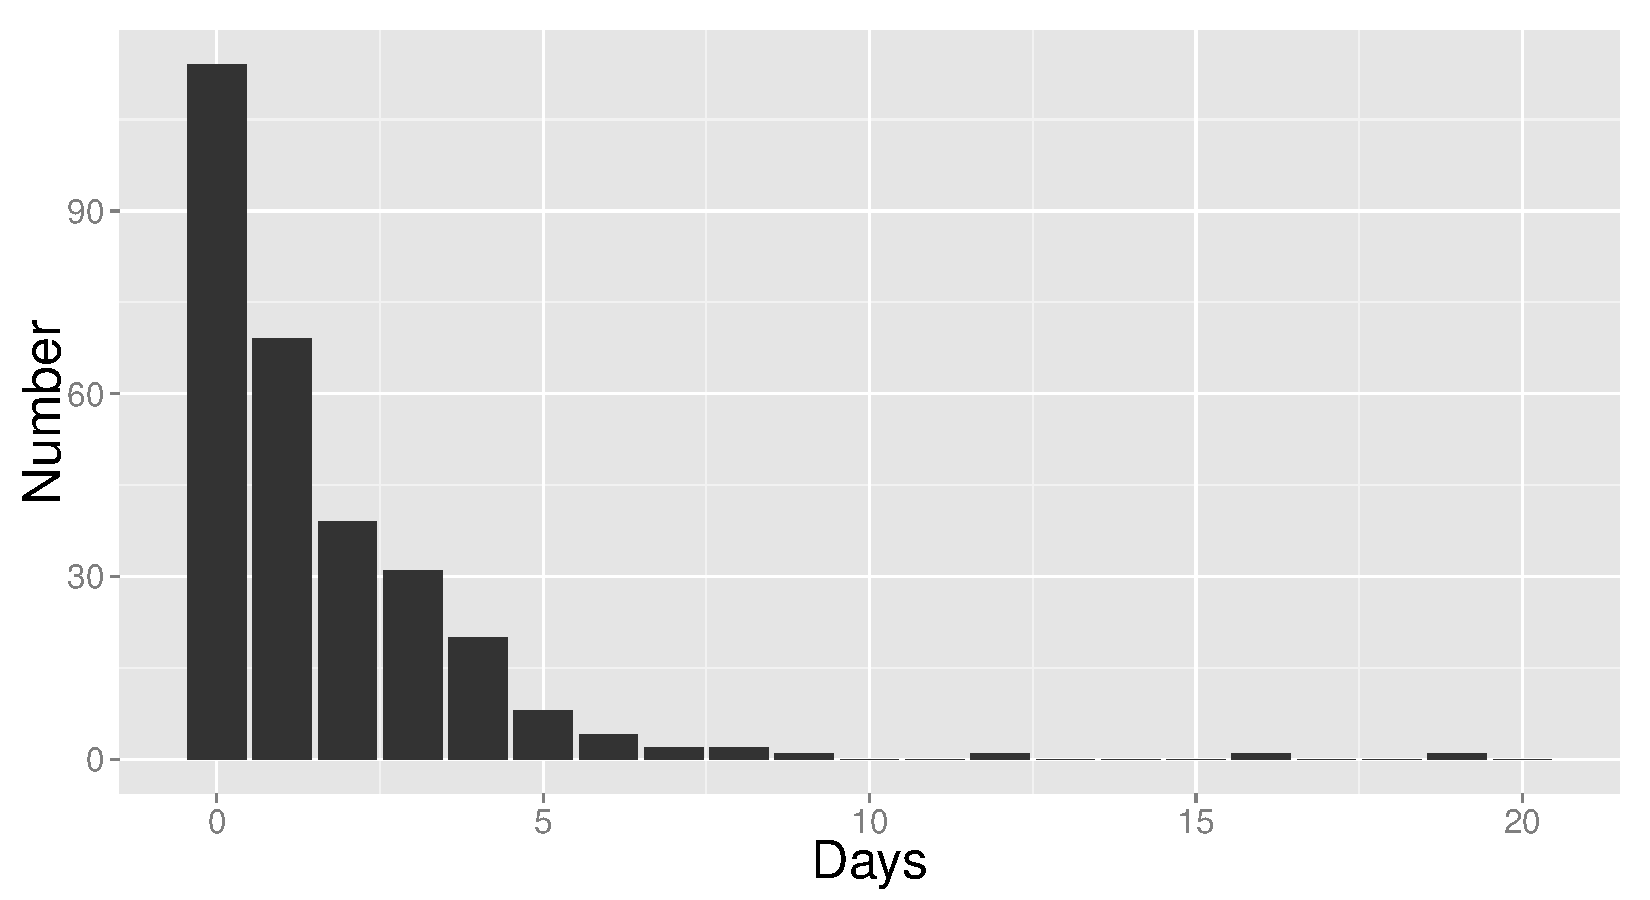
\includegraphics{draftfinalreport-047}
\end{center}
\caption{Number of measles cases attending hospital and stay duration from 2000--2014}
\label{fig:hosp}
\end{figure}

Nearly 40\% (114/293) of the cases did not spend a night in the hospital, while approximately one-quarter (69/293) spent 1 night and more than three-quarters (222/293) spent less than three nights in the hospital. Only eight cases spent a week or more in the hospital. Due to the small number of cases spending a week or more in the hospital, the regression analysis to determine the association between cost of hospitalisation was limited to the 285 cases hospitalised for seven or fewer days. The number of cases, length of hospital stay, cost, cost per case and cost per day for patients with measles as the primary diagnosis, by year and gender for 2000--2014 appear in Table~\ref{table:cases}.


\begin{table}\small
\caption{Number of cases, length of hospital stay, cost, cost per case and cost per day for patients with measles as the primary diagnosis, by year and gender, 2000--2014}
%latex.default(costtable4, file = "", table.env = FALSE, rowname = NULL)%
\begin{center}
\begin{tabular}{lllrrl}
\hline\hline
\multicolumn{1}{c}{Year}&\multicolumn{1}{c}{Gender}&\multicolumn{1}{c}{Cost}&\multicolumn{1}{c}{Cases}&\multicolumn{1}{c}{Length.of.stay}&\multicolumn{1}{c}{Cost.per.case}\tabularnewline
\hline
2000&F&4,296&$  2$&$  4$&2,148\tabularnewline
&M&4,554&$  4$&$  9$&1,139\tabularnewline
&Total&8,850&$  6$&$ 13$&1,475\tabularnewline
2001&F&3,740&$  5$&$  5$&748\tabularnewline
&M&7,527&$  8$&$ 13$&941\tabularnewline
&Total&11,267&$ 13$&$ 18$&867\tabularnewline
2002&F&924&$  2$&$  0$&462\tabularnewline
&M&2,945&$  3$&$  2$&982\tabularnewline
&Total&3,869&$  5$&$  2$&774\tabularnewline
2003&F&9,766&$  8$&$ 12$&1,221\tabularnewline
&M&475&$  1$&$  0$&475\tabularnewline
&Total&10,241&$  9$&$ 12$&1,138\tabularnewline
2004&F&1,437&$  1$&$  2$&1,437\tabularnewline
&M&3,328&$  3$&$  3$&1,109\tabularnewline
&Total&4,765&$  4$&$  5$&1,191\tabularnewline
2005&F&0&$  0$&$  0$&0\tabularnewline
&M&5,111&$  3$&$ 11$&1,704\tabularnewline
&Total&5,111&$  3$&$ 11$&1,704\tabularnewline
2006&F&0&$  0$&$  0$&0\tabularnewline
&M&602&$  1$&$  0$&602\tabularnewline
&Total&602&$  1$&$  0$&602\tabularnewline
2007&F&1,930&$  1$&$  3$&1,930\tabularnewline
&M&81,046&$  4$&$ 22$&20,262\tabularnewline
&Total&82,977&$  5$&$ 25$&16,595\tabularnewline
2008&F&714&$  1$&$  0$&714\tabularnewline
&M&2,324&$  2$&$  1$&1,162\tabularnewline
                    &Total&3,038&$  3$&$  1$&1,013\tabularnewline
2009&F&11,953&$  7$&$ 15$&1,708\tabularnewline
&M&28,830&$ 22$&$ 23$&1,310\tabularnewline
                    &Total&40,782&$ 29$&$ 38$&1,406\tabularnewline
2010&F&5,884&$  4$&$  5$&1,471\tabularnewline
&M&817&$  1$&$  0$&817\tabularnewline
                    &Total&6,701&$  5$&$  5$&1,340\tabularnewline
2011&F&103,460&$ 66$&$ 86$&1,568\tabularnewline
&M&101,842&$ 66$&$103$&1,543\tabularnewline
                    &Total&205,303&$132$&$189$&1,555\tabularnewline
2012&F&13,054&$  8$&$  6$&1,632\tabularnewline
&M&15,486&$ 11$&$  6$&1,408\tabularnewline
                    &Total&28,540&$ 19$&$ 12$&1,502\tabularnewline
2013&F&1,800&$  1$&$  2$&1,800\tabularnewline
&M&3,530&$  3$&$  4$&1,177\tabularnewline
                    &Total&5,330&$  4$&$  6$&1,333\tabularnewline
2014&F&55,633&$ 21$&$ 46$&2,649\tabularnewline
&M&77,014&$ 34$&$ 87$&2,265\tabularnewline
&Total&132,647&$ 55$&$133$&2,412\tabularnewline
2000-2014&      F&335,431&$166$&$284$&2,021\tabularnewline
&     M&214,591&$127$&$186$&1,690\tabularnewline
&   TOTAL&550,022&$293$&$470$&1,877\tabularnewline
\hline
\end{tabular}\end{center}\label{table:cases}
 \centering
 \begin{tablenotes}
      \small
      \item As of 7 August, 2014.
    \end{tablenotes}
\end{table}

Regression analyses showed statistically significant associations between cost of hospitalisation and three variables, length of hospitalisation, case age and year of case, and a less strong association with case gender (Table~\ref{table:regression}). Results showed the expected hospitalisation costs in 2000 of a female measles patient who did not stay overnight in the hospital was \$582.  The cost was \$256 less if the case were a male. It increased of approximately \$406 per night of hospitalisation and \$64 per year over the time period of 2000--2014. The cost of a case decreased with the age of the patient by approximately \$8 per year of case age.


\begin{table}
\caption{Regression results ($R^{2}_\textsf{adj} = 0.43$, p-value $<0.001$) for measles hospitalisation cost based on length of stay (days), gender, case age and year of case ($n=288$) in New Zealand, 2000 -- 2014}
%latex.default(costtable5, file = "", table.env = FALSE, rowname = NULL)%
\begin{center}
\begin{tabular}{lrl}
\hline\hline
\multicolumn{1}{c}{Variable}&\multicolumn{1}{c}{Coefficient}&\multicolumn{1}{c}{P.value}\tabularnewline
\hline
Intercept&$ 581.39$&\textless  0.001\tabularnewline
Length of stay (nights)&$ 406.07$&\textless  0.001\tabularnewline
Gender (0 = F, 1 = M)&$-255.98$&0.006\tabularnewline
Case age (years)&$  -8.23$&0.007\tabularnewline
Year of case (vs. 2000)&$  64.35$&\textless  0.001\tabularnewline
\hline
\end{tabular}\end{center}\label{table:regression}
\end{table}

Wages lost due to measles were calculated for the period January 2008 -- August 2014. Calculations were based on the assumption that 5 days of work were lost for each case; however, individuals under 15 years of age were not assumed to be employed and therefore did not suffer an income loss. If the case were less than 20 years of age, it was assumed there was an income loss of 5 days for the care giver, in addition to the wage loss of the case if 15--19 years of age. Total wage lost for the 247 cases and care givers was estimated to be \$210,436. This consisted of \$107,820 for the cases and \$102,616 for the care giver, but did not include wage losses for cases under 15 years of age. Overall, the cost per case from 2008--2014 was estimated to be \$2,562 (\$852 in forgone wages and \$1,710 in hospital costs).

%%%%%%%% REVISE

This final figure brings an approximate estimate of \$786,479 for the current 2014 outbreak, which is comprised of earnings lost, case management and hospitalisation costs.


\subsection{Benefit--cost analyses methods}
To estimate the benefits from additional vaccinations, as estimated from the above modelling section (Section~\ref{sec:epidemic_modelling}), we did several things. Primarily, we simulated 1000 measles outbreaks using the estimated $R_v$ distribution from (Section~\ref{sec:epidemic_modelling}) in the estimated susceptible population of naive New Zealanders (Figure~\ref{fig:naive}). We assumed recovery from infection led to immunity and thus constantly reduced the population size by the number recovered. We used these values of numbers of predicted cases and the cost figures above to estimate what the cost of not vaccinating additional populations would be. We also simulated what we might expect measles outbreaks to look like following introductions in the population, given that $R_v$ would be one, though where our estimates for $R_v$ are already < 1, we use this. We can therefore estimate the number of cases prevented, and the savings made from the additional vaccinations. We then use the costs of the catch up vaccination schemes, the costs of the expected measles-related costs due to constant introduction of measles despite increased population immunity, and the savings from reduced measles cases to work out the benefit--cost ratio ((B/C), where a B/C ratio > 1 means that the program benefits exceed their costs. A B/C value less than one suggests the costs are higher than the economic benefits. Lastly, benefits were assessed over a 10--year time period, using a discounting rate of 3\% discount per year for the costs, as is common for healthcare discounting \citep{honeycutt6}:

\begin{equation} \label{eq:disc}
\textit{present value} = \sum \textit{future value}_y_r * (1/(1+\textit{discount rate})^{yr}
  \end{equation}
Where $_y_r$ is the year 0 (current) through to 9 (ten years into the future).

Our estimates for the numbers of measles cases are highly variable: if $R_v$ were greater than one, either the measles outbreak would take off and all the susceptible New Zealand population would become infected during the outbreak, or the epidemic it would stutter after a few infects and fail to cause a large epidemic due to stochasticity. We used the average of 1000 simulations to estimate the mean of these stochastic simulations for our benefit--cost analysis. However, these simulations assume a homogeneously mixed population and thus give large epidemic sizes once the epidemic gets beyond the initial stuttering infection chains and this assumption is discussed below. However, to address this, we not only use $R_v$ values of 1 in simulation models to estimate predicted outbreak sizes, but we also compared our results to those using the mean number of measles cases seen in New Zealand per year since 1997. This was 220 cases per year.

The numbers of susceptible people to vaccinate in New Zealand, assuming a homogeneously mixed population and using the upper 95\% confidence limits of our $R_v$ estimates (Section~\ref{sec:epidemic_modelling}) are shown in Figure~\ref{fig:numvac}.


\begin{figure}
     \centering
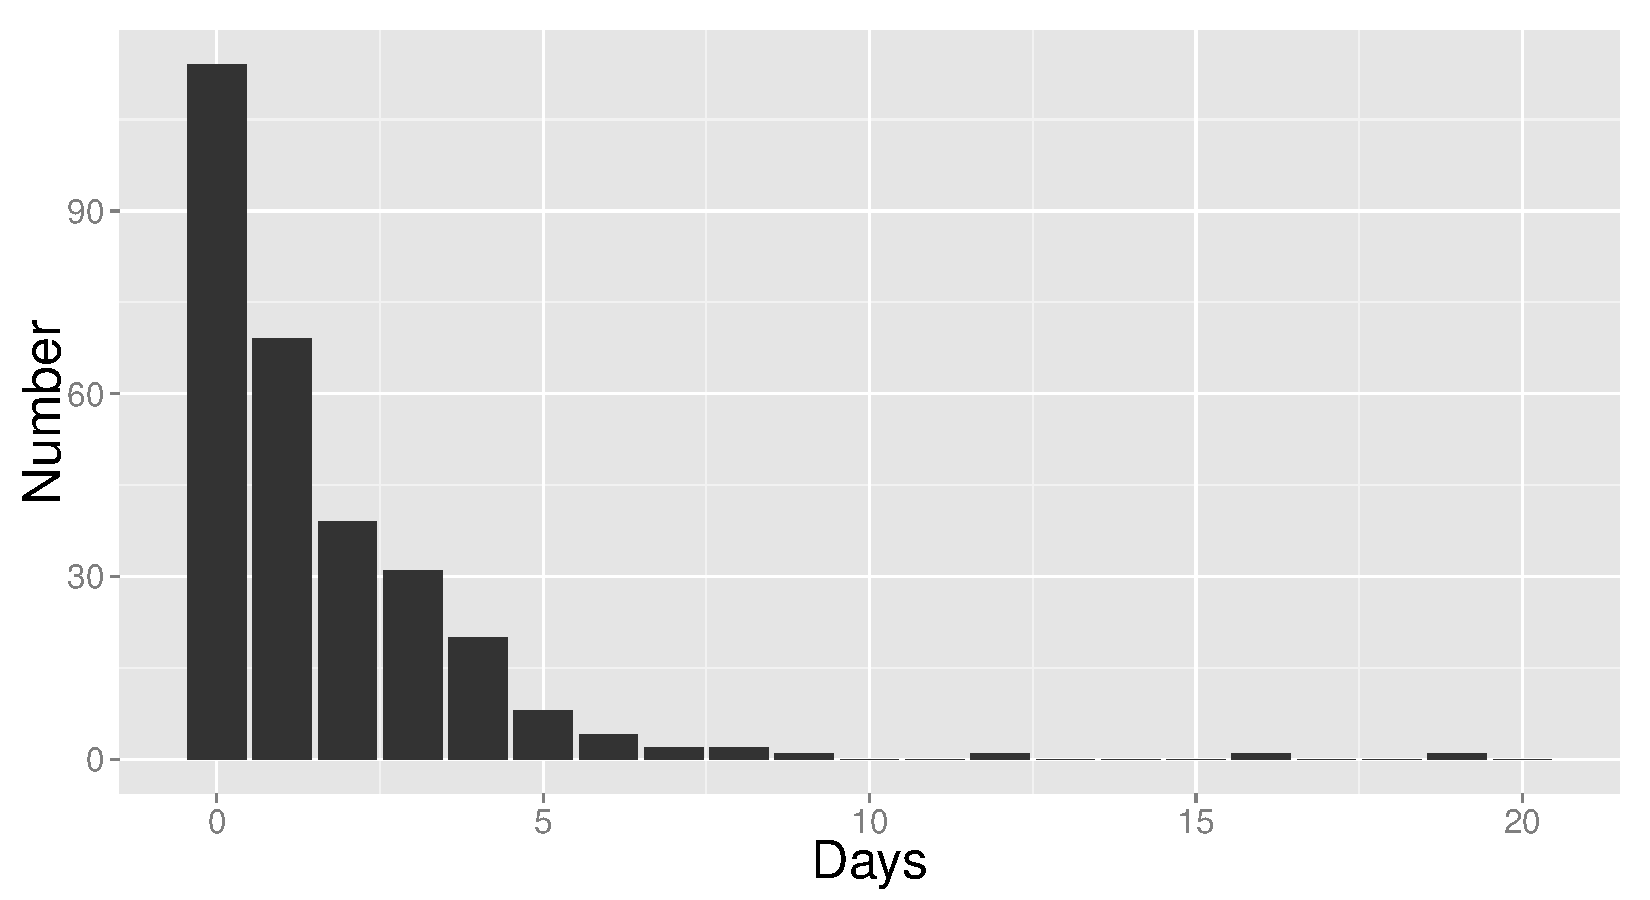
\includegraphics{draftfinalreport-053}
     \caption{The estimated proportion of the currently naive New Zealand population requiring additional vaccination given alternative $R_v$ values to reduce the $R_v$ to one (Section~\ref{sec:epidemic_modelling}, Tables~\ref{tab:cost_sim} and ~\ref{tab:cost_ave}}
     \label{fig:numvac}
\end{figure}

The expected number of cases in New Zealand, assuming homogenous mixing in a naive population of 11\% of the population (the current status) and assuming measles $R_v$ were 1 is shown in Figure~\ref{fig:sim} and Figure~\ref{fig:sim1}. These simulations show that even in scenarios when $R_v$ is one, and thus stochastically should fail to persist (i.e. become endemic), large outbreaks can occur due to stochastic processes. Though the median value from 1000 simulations is low (2 cases), and thus most measles introductions will be single cases or lead to minor outbreaks, in this modelling exercise the mean value was 151 cases and the maximum nearly 25,000 cases.


\begin{figure}
     \centering
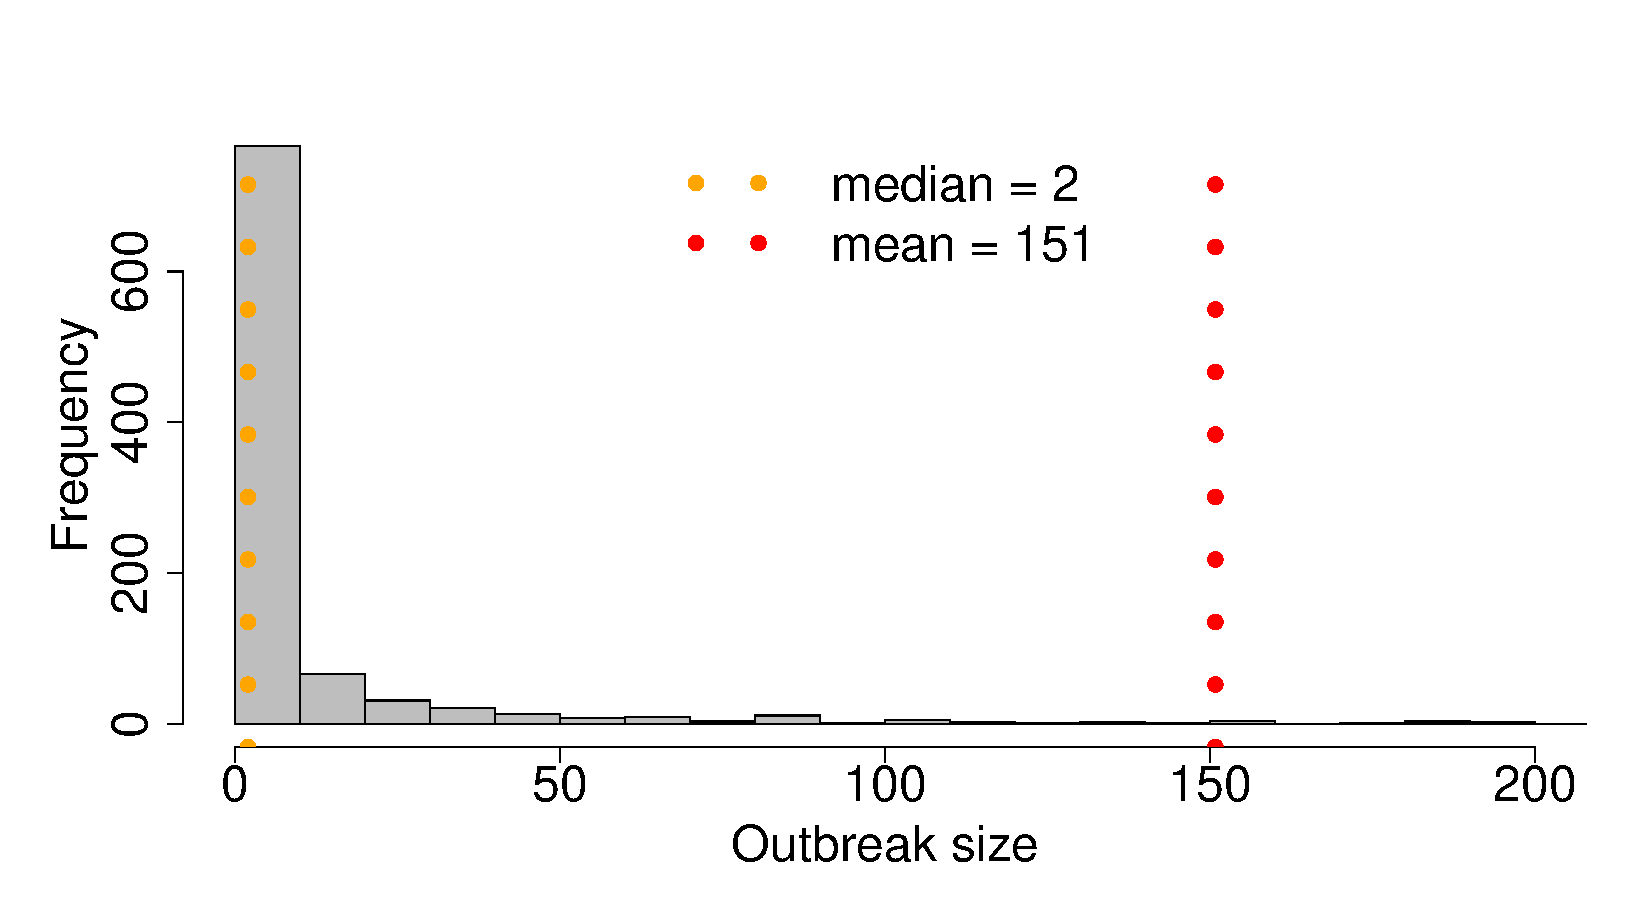
\includegraphics{draftfinalreport-055}
     \caption{A subset of the expected number of measles cases from 1000 simulations of a model (Section~\ref{sec:epidemic_modelling}) in a homogeneously mixed population in New Zealand with 11\% susceptible to measles infection using an $R_v$ =1. The full distribution of results can be seen in Figure~\ref{fig:sim1}}
     \label{fig:sim}
\end{figure}

\begin{figure}
     \centering
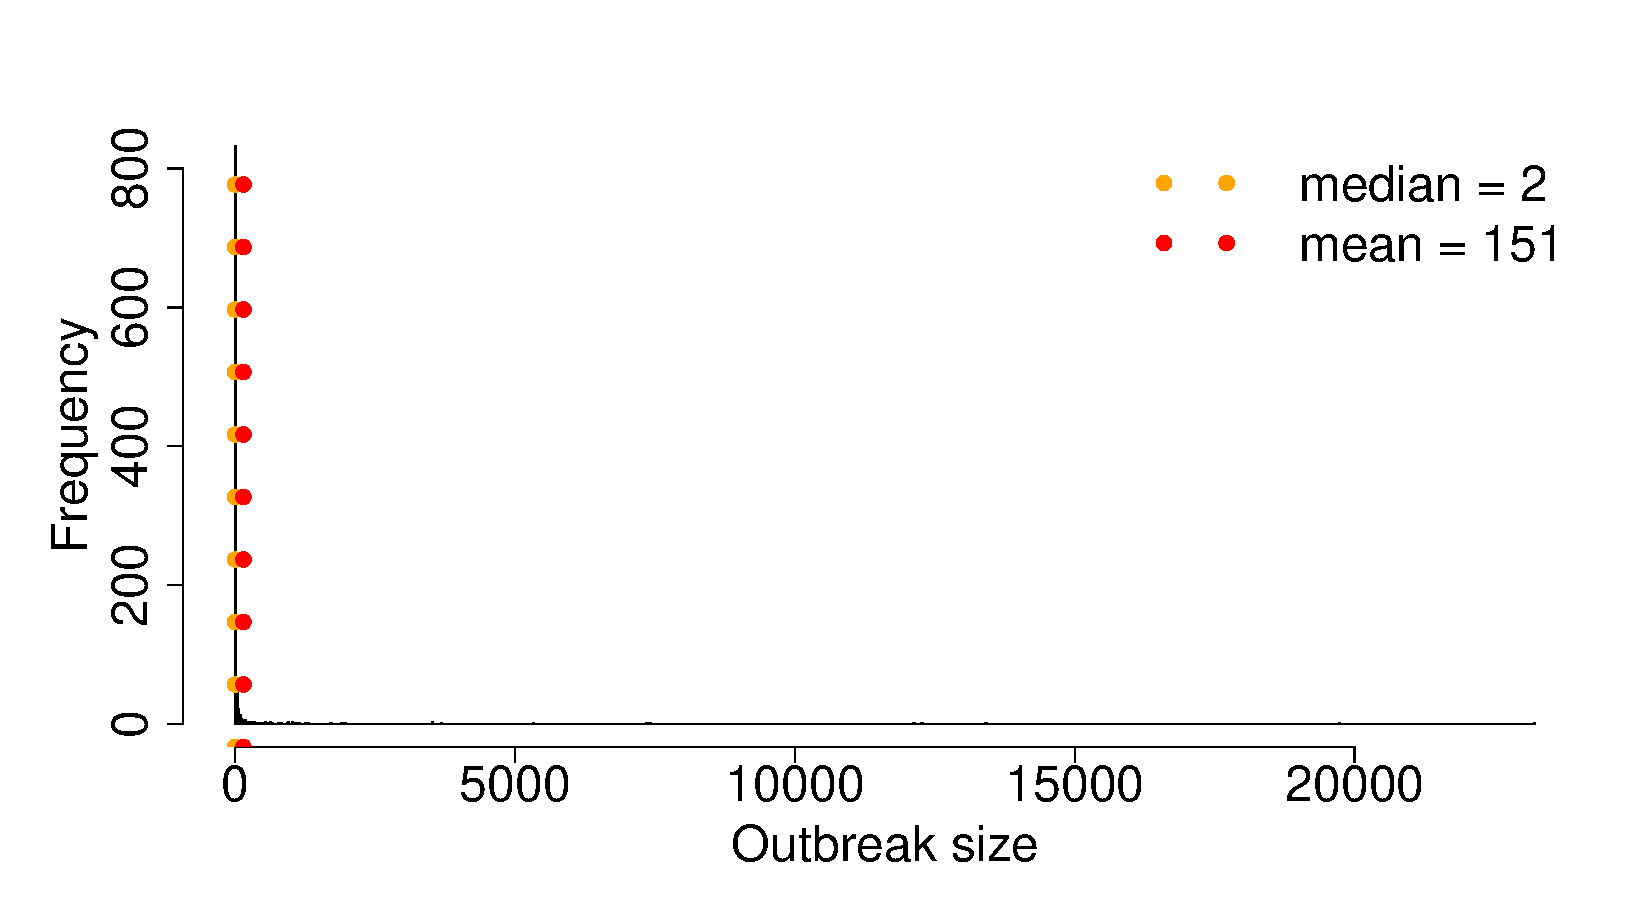
\includegraphics{draftfinalreport-056}
     \caption{The distribution of the expected number of measles cases from 1000 simulations of a model (Section~\ref{sec:epidemic_modelling}) in a homogeneously mixed population in New Zealand with 11\% susceptible to measles infection using an $R_v$ =1, showing the rare but possible large epidemic sizes possible. A subset of the distribution of results can be seen in Figure~\ref{fig:sim}}
     \label{fig:sim1}
\end{figure}

For the cost analyses we used the values from the above cost section (Section~\ref{sub:cost_benefit}). Specifically, we used the average cost of a case for the analyses to be \$852 lost in wages and \$1710 in hospitalisation costs for those attending hospital, with 17\% of cases predicted to be hospitalised (Table~\ref{table:hosp}). We estimated there would be approximately one introduction of measles per year (Section~\ref{sub:risk_analyses}). We provide two costs for measles vaccinations for our cost analyses, \$20 and \$50, based on US literature.


\subsection{Cost analysis discussion}
The results presented here are based on available data. While some of the data are complete and detailed, this is not true of all the data. In order to perform an accurate analysis of the current measles outbreak in New Zealand, more complete data are needed. For instance, age, gender, ethnicity, year of discharge, length of stay and estimated cost data are available for cases reported by publicly funded hospitals. In addition to this information, similar data would be needed for cases occurring outside the period 2011--2013 at publicly funded hospitals. In addition, similar data would be needed for non-publicly funded hospitals, e.g. private clinics. Other factors that we aim to investigate are whether or not a linear term for case age is appropriate, or what if any interaction there might be between age and length of stay in hospital.

Detailed measles outbreak management costs were provided for the period of January 1 -- March 9, 2014. Similar data are needed for the period preceding 2014. If detailed data, such as that provided for early 2014, are not available, aggregated data would be acceptable. However, it is unrealistic to assume that these costs would be linearly related with the number of measles cases, making it difficult to extrapolate these costs outside the reported period for 2014. As other studies have demonstrated, direct costs required to manage measles are not linear.

In other outbreaks, the average cost per measles case was estimated to be US\$254, US\$276, and US\$307 for Canada, the Netherlands, and the UK, respectively (Carabin, et al., 2002). This and other findings will be compared and contrasted with New Zealand costs, once more complete New Zealand data are made available.
The containment of a single case (also 2 secondary cases) of measles in 2004 in Iowa, USA was estimated to cost US\$142,542. In this outbreak, more than 2500 hours of personnel time were needed to investigate and respond to the outbreak (Dayan et al., 2005). They estimated direct costs per case to be less than US\$500. 
The annual cost for long-term care of people with moderate of severe mental retardation over a period of 50 years is estimated at US\$31,059 and US\$78,448, respectively \citep{prouty1}. In 2000 expenditures for care in large state mental retardation/developmental disabilities (MR/DD) facilities continued to increase and reached a national annual average of US\$113,864 per person. In 2000 the average annual expenditures for care in large state MR/DD facilities were \$113,864. The cost of a case of measles was estimated to range from \$71 (no complications and no hospitalisation) to \$29,556 (encephalitis and hospitalisation for 8.7 days). They estimated the annual cost of measles in the US with its vaccination program to be \$1,234,083 (52.5\% direct cost and 47.5\% indirect cost) \citep{zhou4}.


\subsection{Benefit--cost analyses results}

\begin{sidewaystable}[htbp]  
  \centering  
  \begin{raggedright}
  \caption{Cost benefit analyses using simulated epidemic sizes}  
  \label{tab:cost_sim}
   \begin{threeparttable}[b] \tiny
    \begin{tabular}{p{0.8cm}p{0.8cm}p{0.8cm}p{0.9cm}p{0.9cm}p{0.8cm}p{0.9cm}p{0.9cm}p{0.9cm}p{0.9cm}p{0.9cm}p{0.9cm}p{0.9cm}p{0.9cm}p{0.9cm}p{0.9cm}p{0.9cm}p{0.9cm}p{0.9cm}p{0.9cm}p{0.9cm}}  
    \toprule  
   
Years $R_v$ estimated from & $R_v$ range &  $R_v$  for simulations &	Additional vaccines required to reduce $R_v$ to 1 &	Costs per vaccine (\$) &	Present value of discounted vaccination costs (\$) &	Mean total cases in over 10 years without additional vaccination \dagger&	Total hospitalised cases\sym{*}	& Total undiscounted case costs without additional vaccination (\$)\sym{**} &	Present value of discounted case costs of baseline program (\$)(Equation~\ref{eq:pc}) &	Mean epidemic size in immune pop over 10 years with $R_v$ = 1 \dagger &	Total cases over 10 years following additional vaccination\sym{***} &	Total hospitalised cases following additional vaccination &	Total costs for cases assuming supplemental vaccination (\$) &	Total cases reduce by vaccination alternative vs baseline &	Present value of discounted benefits from reducing cases with supplemental vaccination program	& Discounted net benefit of supplemental vaccination program &	Benefit--cost ratio\\
\midrule
2009-2014 &	0.92-1.19	& 0.92	& 0	    & na	  & 0	      & 130	    & 22  	& 148551	  & 130519	  & 13	& 130	  & 22	& 148551	& 0	      & 0	        & 0	        & na \\
2009-2014	& 0.92-1.19	& 1.19	& 80000	& 20	  & 1600000	& 128901	& 21913	& 147295173	& 129415143	& 145	& 1450	& 247	& 1656915	& 127451	& 127959360	& 126359360	& 79.97 \\
2009-2014	& 0.92-1.19	& 1.19	& 80000	& 50	  & 4000000	& 128901	& 21913	& 147295173	& 129415143	& 145	& 1450	& 247	& 1656915	& 127451	& 127959360	& 123959360	& 31.99 \\
2013-2014	& 1.82-2.13	& 1.82	& 208153	& 20	& 4163060	& 340032	& 57805	& 388554566	& 341388274	& 116	& 1160	& 197	& 1325532	& 338872	& 340223647	& 336060587	& 81.72 \\
2013-2014	& 1.82-2.13	& 1.82	& 208153	& 50	& 10407650& 340032	& 57805	& 388554566	& 341388274	& 116	& 1160	& 197	& 1325532	& 338872	& 340223647	& 329815997	& 32.69 \\
2013-2014	& 1.82-2.13	& 2.13	& 252561	& 20	& 5051220	& 382074	& 64953	& 436595960	& 383597966	& 116	& 1160	& 197	& 1325532	& 380914	& 382433339	& 377382119	& 75.71 \\
2013-2014	& 1.82-2.13	& 2.13	& 252561	& 50	& 12628050& 382074	& 64953	& 436595960	& 383597966	& 116	& 1160	& 197	& 1325532	& 380914	& 382433339	& 369805289	& 30.28 \\

\end{raggedright}
\bottomrule  
    \end{tabular}%  
    \begin{tablenotes}\footnotesize  
        \item $\dagger$ {1000 simulations}
        \item \sym{*} Proportion of cases hospitalised 0.17
        \item \sym{**} Wage losses per case = \$852 and cost per hospitalised case = \$1710
        \item \sym{***} Based on 10 introductions of measles, one per year
      \end{tablenotes}  
    \end{threeparttable}  
\end{sidewaystable}

\normalsize

\begin{sidewaystable}[htbp]  
  \centering  
  \begin{raggedright}
  \caption{Cost benefit analyses using historic epidemic sizes since 1997}  
  \label{tab:cost_ave}
   \begin{threeparttable}[b] \tiny
    \begin{tabular}{p{0.8cm}p{0.8cm}p{0.8cm}p{0.9cm}p{0.9cm}p{0.8cm}p{0.9cm}p{0.9cm}p{0.9cm}p{0.9cm}p{0.9cm}p{0.9cm}p{0.9cm}p{0.9cm}p{0.9cm}p{0.9cm}p{0.9cm}p{0.9cm}p{0.9cm}p{0.9cm}p{0.9cm}}  
    \toprule  
Years $R_v$ estimated from & $R_v$ range &  $R_v$  for simulations &	Additional vaccines required to reduce $R_v$ to 1 &	Costs per vaccine (\$) &	Present value of discounted vaccination costs (\$) &	Mean total cases in over 10 years without additional vaccination \ddagger &	Total hospitalised cases\sym{*}	& Total undiscounted case costs without additional vaccination (\$)\sym{**} &	Present value of discounted case costs of baseline program (\$)(Equation~\ref{eq:pc}) &	Mean epidemic size in immune pop over 10 years with $R_v$ = 1 \dagger &	Total cases over 10 years following additional vaccination\sym{***} &	Total hospitalised cases following additional vaccination &	Total costs for cases assuming supplemental vaccination (\$) &	Total cases reduce by vaccination alternative vs baseline &	Present value of discounted benefits from reducing cases with supplemental vaccination program	& Discounted net benefit of supplemental vaccination program &	Benefit--cost ratio\\
\midrule

2009-2014	& 0.92-1.19	& 0.92	& 0	      & na	& 0	      & 130	  & 22	& 148551	  & 130519	& 13	& 130	  & 22	& 148551	& 0	  & 0	      & 0	        & na \\
2009-2014	& 0.92-1.19	& 1.19	& 80000	  & 20	& 1600000	& 2200	& 374	& 2513940	  & 2208775	& 145	& 1450	& 247	& 1656915	& 750	& 752991	& -847009	  & 0.47 \\
2009-2014	& 0.92-1.19	& 1.19	& 80000	  & 50	& 4000000	& 2200	& 374	& 2513940	  & 2208775	& 145	& 1450	& 247	& 1656915	& 750	& 752991	& -3247009	& 0.19 \\ 
2013-2014	& 1.82-2.13	& 1.82	& 208153	& 20	& 4163060	& 2200	& 374	& 2513940	  & 2208775	& 116	& 1160	& 197	& 1325532	& 1040& 1044148	& -3118912	& 0.25 \\
2013-2014	& 1.82-2.13	& 1.82	& 208153	& 50	& 10407650& 2200	& 374	& 2513940	  & 2208775	& 116	& 1160	& 197	& 1325532	& 1040& 1044148	& -9363502	& 0.10 \\
2013-2014	& 1.82-2.13	& 2.13	& 252561	& 20	& 5051220	& 2200	& 374	& 2513940	  & 2208775	& 116	& 1160	& 197	& 1325532	& 1040& 1044148	& -4007072	& 0.21 \\
2013-2014	& 1.82-2.13	& 2.13	& 252561	& 50	& 12628050& 2200	& 374	& 2513940	  & 2208775	& 116	& 1160	& 197	& 1325532	& 1040& 1044148	& -11583902	& 0.08 \\
\end{raggedright}
\bottomrule  
    \end{tabular}%  
    \begin{tablenotes}\footnotesize  
        \item $\ddagger$ Based on average number of cases per year in New Zealand from 1997 onward
        \item $\dagger$ {1000 simulations}
        \item \sym{*} Proportion of cases hospitalised 0.17
        \item \sym{**} Wage losses per case \$852 and cost per hospitalised case \$1710
        \item \sym{***} Based on 10 introductions of measles, one per year
      \end{tablenotes}  
    \end{threeparttable}  
\end{sidewaystable}

\normalsize


\begin{sidewaystable}\small
\caption{Cost benefit analyses with 20 dollars per vaccine}
%latex.default(costtable20, file = "", table.env = FALSE, rowname = NULL)%
\begin{center}
\begin{tabular}{lrrrrrrrrrr}
\hline\hline
\multicolumn{1}{c}{DHB}&\multicolumn{1}{c}{Vaccines}&\multicolumn{1}{c}{Vac.costs}&\multicolumn{1}{c}{Wage.loss}&\multicolumn{1}{c}{Management}&\multicolumn{1}{c}{Hospitalised}&\multicolumn{1}{c}{Hospitalisation}&\multicolumn{1}{c}{Costs}&\multicolumn{1}{c}{Outbreak}&\multicolumn{1}{c}{OB.costs}&\multicolumn{1}{c}{Benefit.cost}\tabularnewline
\hline
Auckland&$17920$&$358400$&$26547468$&$55010965$&$5297$&$9057921$&$79616516$&$ 82$&$209524$&$140.19$\tabularnewline
Bay of Plenty&$ 4585$&$ 91700$&$ 7188324$&$14895456$&$1434$&$2452636$&$21557962$&$ 71$&$181417$&$ 78.93$\tabularnewline
Canterbury&$13687$&$273740$&$21040140$&$43598824$&$4198$&$7178837$&$63099902$&$ 62$&$158420$&$146.01$\tabularnewline
Capital and Coast&$10461$&$209220$&$15679356$&$32490349$&$3129$&$5349752$&$47022778$&$ 96$&$245296$&$103.46$\tabularnewline
Counties Manukau&$18880$&$377600$&$28033356$&$58089983$&$5594$&$9564902$&$84072731$&$ 50$&$127758$&$166.36$\tabularnewline
Hawke's Bay&$ 3751$&$ 75020$&$ 5832792$&$12086558$&$1164$&$1990132$&$17492688$&$ 56$&$143089$&$ 80.20$\tabularnewline
Hutt Valley&$ 4388$&$ 87760$&$ 6676272$&$13834395$&$1332$&$2277925$&$20022305$&$ 86$&$219745$&$ 65.11$\tabularnewline
Lakes&$ 2886$&$ 57720$&$ 4423584$&$ 9166434$&$ 883$&$1509314$&$13266438$&$ 62$&$158420$&$ 61.38$\tabularnewline
MidCentral&$ 4628$&$ 92560$&$ 7112496$&$14738327$&$1419$&$2426764$&$21330552$&$ 75$&$191638$&$ 75.06$\tabularnewline
Nelson Marlborough&$ 2356$&$ 47120$&$ 3758172$&$ 7787585$&$ 750$&$1282278$&$11270851$&$ 90$&$229965$&$ 40.68$\tabularnewline
Northland&$ 3071$&$ 61420$&$ 4846176$&$10042118$&$ 967$&$1653502$&$14533802$&$ 70$&$178862$&$ 60.49$\tabularnewline
South Canterbury&$  893$&$ 17860$&$ 1429656$&$ 2962496$&$ 285$&$ 487795$&$ 4287574$&$ 72$&$183972$&$ 21.24$\tabularnewline
Southern&$ 8371$&$167420$&$12877980$&$26685411$&$2570$&$4393931$&$38621382$&$102$&$260627$&$ 90.23$\tabularnewline
Tairawhiti&$ 1359$&$ 27180$&$ 2071212$&$ 4291911$&$ 413$&$ 706692$&$ 6211616$&$ 47$&$120093$&$ 42.18$\tabularnewline
Taranaki&$ 2899$&$ 57980$&$ 4488486$&$ 9290019$&$ 895$&$1529663$&$13449923$&$ 68$&$173752$&$ 58.04$\tabularnewline
Waikato&$11331$&$226620$&$17291792$&$35747682$&$3442$&$5886094$&$51772645$&$ 95$&$242741$&$110.30$\tabularnewline
Wairarapa&$  720$&$ 14400$&$ 1150830$&$ 2376352$&$ 229$&$ 391282$&$ 3442806$&$ 59$&$150755$&$ 20.85$\tabularnewline
Waitemata&$17291$&$345820$&$26342544$&$54331250$&$5232$&$8946002$&$78740929$&$ 70$&$178862$&$150.07$\tabularnewline
West Coast&$  685$&$ 13700$&$ 1084105$&$ 2233347$&$ 215$&$ 367736$&$ 3237846$&$ 50$&$127758$&$ 22.89$\tabularnewline
Whanganui&$ 1378$&$ 27560$&$ 2170740$&$ 4466695$&$ 430$&$ 735471$&$ 6477915$&$ 58$&$148200$&$ 36.86$\tabularnewline
\hline
\end{tabular}\end{center}\label{table:cost20}
\end{sidewaystable}


\begin{sidewaystable}\small
\caption{Cost benefit analyses with 50 dollars per vaccine}
%latex.default(costtable50, file = "", table.env = FALSE, rowname = NULL)%
\begin{center}
\begin{tabular}{lrrrrrrrrrr}
\hline\hline
\multicolumn{1}{c}{DHB}&\multicolumn{1}{c}{Vaccines}&\multicolumn{1}{c}{Vac.costs}&\multicolumn{1}{c}{Wage.loss}&\multicolumn{1}{c}{Management}&\multicolumn{1}{c}{Hospitalised}&\multicolumn{1}{c}{Hospitalisation}&\multicolumn{1}{c}{Costs}&\multicolumn{1}{c}{Outbreak}&\multicolumn{1}{c}{OB.costs}&\multicolumn{1}{c}{Benefit.cost}\tabularnewline
\hline
Auckland&$17920$&$896000$&$26547468$&$55010965$&$5297$&$9057921$&$79616516$&$ 82$&$209524$&$72.02$\tabularnewline
Bay of Plenty&$ 4585$&$229250$&$ 7188324$&$14895456$&$1434$&$2452636$&$21557962$&$ 71$&$181417$&$52.49$\tabularnewline
Canterbury&$13687$&$684350$&$21040140$&$43598824$&$4198$&$7178837$&$63099902$&$ 62$&$158420$&$74.87$\tabularnewline
Capital and Coast&$10461$&$523050$&$15679356$&$32490349$&$3129$&$5349752$&$47022778$&$ 96$&$245296$&$61.20$\tabularnewline
Counties Manukau&$18880$&$944000$&$28033356$&$58089983$&$5594$&$9564902$&$84072731$&$ 50$&$127758$&$78.44$\tabularnewline
Hawke's Bay&$ 3751$&$187550$&$ 5832792$&$12086558$&$1164$&$1990132$&$17492688$&$ 56$&$143089$&$52.91$\tabularnewline
Hutt Valley&$ 4388$&$219400$&$ 6676272$&$13834395$&$1332$&$2277925$&$20022305$&$ 86$&$219745$&$45.59$\tabularnewline
Lakes&$ 2886$&$144300$&$ 4423584$&$ 9166434$&$ 883$&$1509314$&$13266438$&$ 62$&$158420$&$43.82$\tabularnewline
MidCentral&$ 4628$&$231400$&$ 7112496$&$14738327$&$1419$&$2426764$&$21330552$&$ 75$&$191638$&$50.42$\tabularnewline
Nelson Marlborough&$ 2356$&$117800$&$ 3758172$&$ 7787585$&$ 750$&$1282278$&$11270851$&$ 90$&$229965$&$32.41$\tabularnewline
Northland&$ 3071$&$153550$&$ 4846176$&$10042118$&$ 967$&$1653502$&$14533802$&$ 70$&$178862$&$43.72$\tabularnewline
South Canterbury&$  893$&$ 44650$&$ 1429656$&$ 2962496$&$ 285$&$ 487795$&$ 4287574$&$ 72$&$183972$&$18.75$\tabularnewline
Southern&$ 8371$&$418550$&$12877980$&$26685411$&$2570$&$4393931$&$38621382$&$102$&$260627$&$56.86$\tabularnewline
Tairawhiti&$ 1359$&$ 67950$&$ 2071212$&$ 4291911$&$ 413$&$ 706692$&$ 6211616$&$ 47$&$120093$&$33.03$\tabularnewline
Taranaki&$ 2899$&$144950$&$ 4488486$&$ 9290019$&$ 895$&$1529663$&$13449923$&$ 68$&$173752$&$42.20$\tabularnewline
Waikato&$11331$&$566550$&$17291792$&$35747682$&$3442$&$5886094$&$51772645$&$ 95$&$242741$&$63.97$\tabularnewline
Wairarapa&$  720$&$ 36000$&$ 1150830$&$ 2376352$&$ 229$&$ 391282$&$ 3442806$&$ 59$&$150755$&$18.43$\tabularnewline
Waitemata&$17291$&$864550$&$26342544$&$54331250$&$5232$&$8946002$&$78740929$&$ 70$&$178862$&$75.46$\tabularnewline
West Coast&$  685$&$ 34250$&$ 1084105$&$ 2233347$&$ 215$&$ 367736$&$ 3237846$&$ 50$&$127758$&$19.99$\tabularnewline
Whanganui&$ 1378$&$ 68900$&$ 2170740$&$ 4466695$&$ 430$&$ 735471$&$ 6477915$&$ 58$&$148200$&$29.84$\tabularnewline
\hline
\end{tabular}\end{center}\label{table:cost50}
\end{sidewaystable}

The benefit--cost results are in Table~\ref{tab:cost_sim} and Table~\ref{tab:cost_ave}. The results in the two tables show two alternative trends. In scenarios where we simulate the expected outbreaks in a homogeneously mixed population and $R_v$ is above 1 the benefits of vaccination are always substantially greater than the costs of the increased supplementary vaccination (Table~\ref{tab:cost_sim}). However, if the previous recent history of cases since 1997 is the \emph{status quo} and what we may expect in the future then the \emph{additional} effort to vaccinate the currently naive population of New Zealand based on $R_v$ estimates that were greater than one is not a cost effective exercise (Table~\ref{tab:cost_ave}).

It is worth noting that vaccination strategies that target the very young (<1 year old) may be less effective, as our analyses of the vaccinated cases suggests a substantial proportion of vaccinated cases that were vaccinated (Figure~\ref{fig:ageandvac}) were vaccinated with a single vaccine at a very young age (Figure~\ref{fig:vaccstat}).

\begin{figure}[h!]
\begin{center}
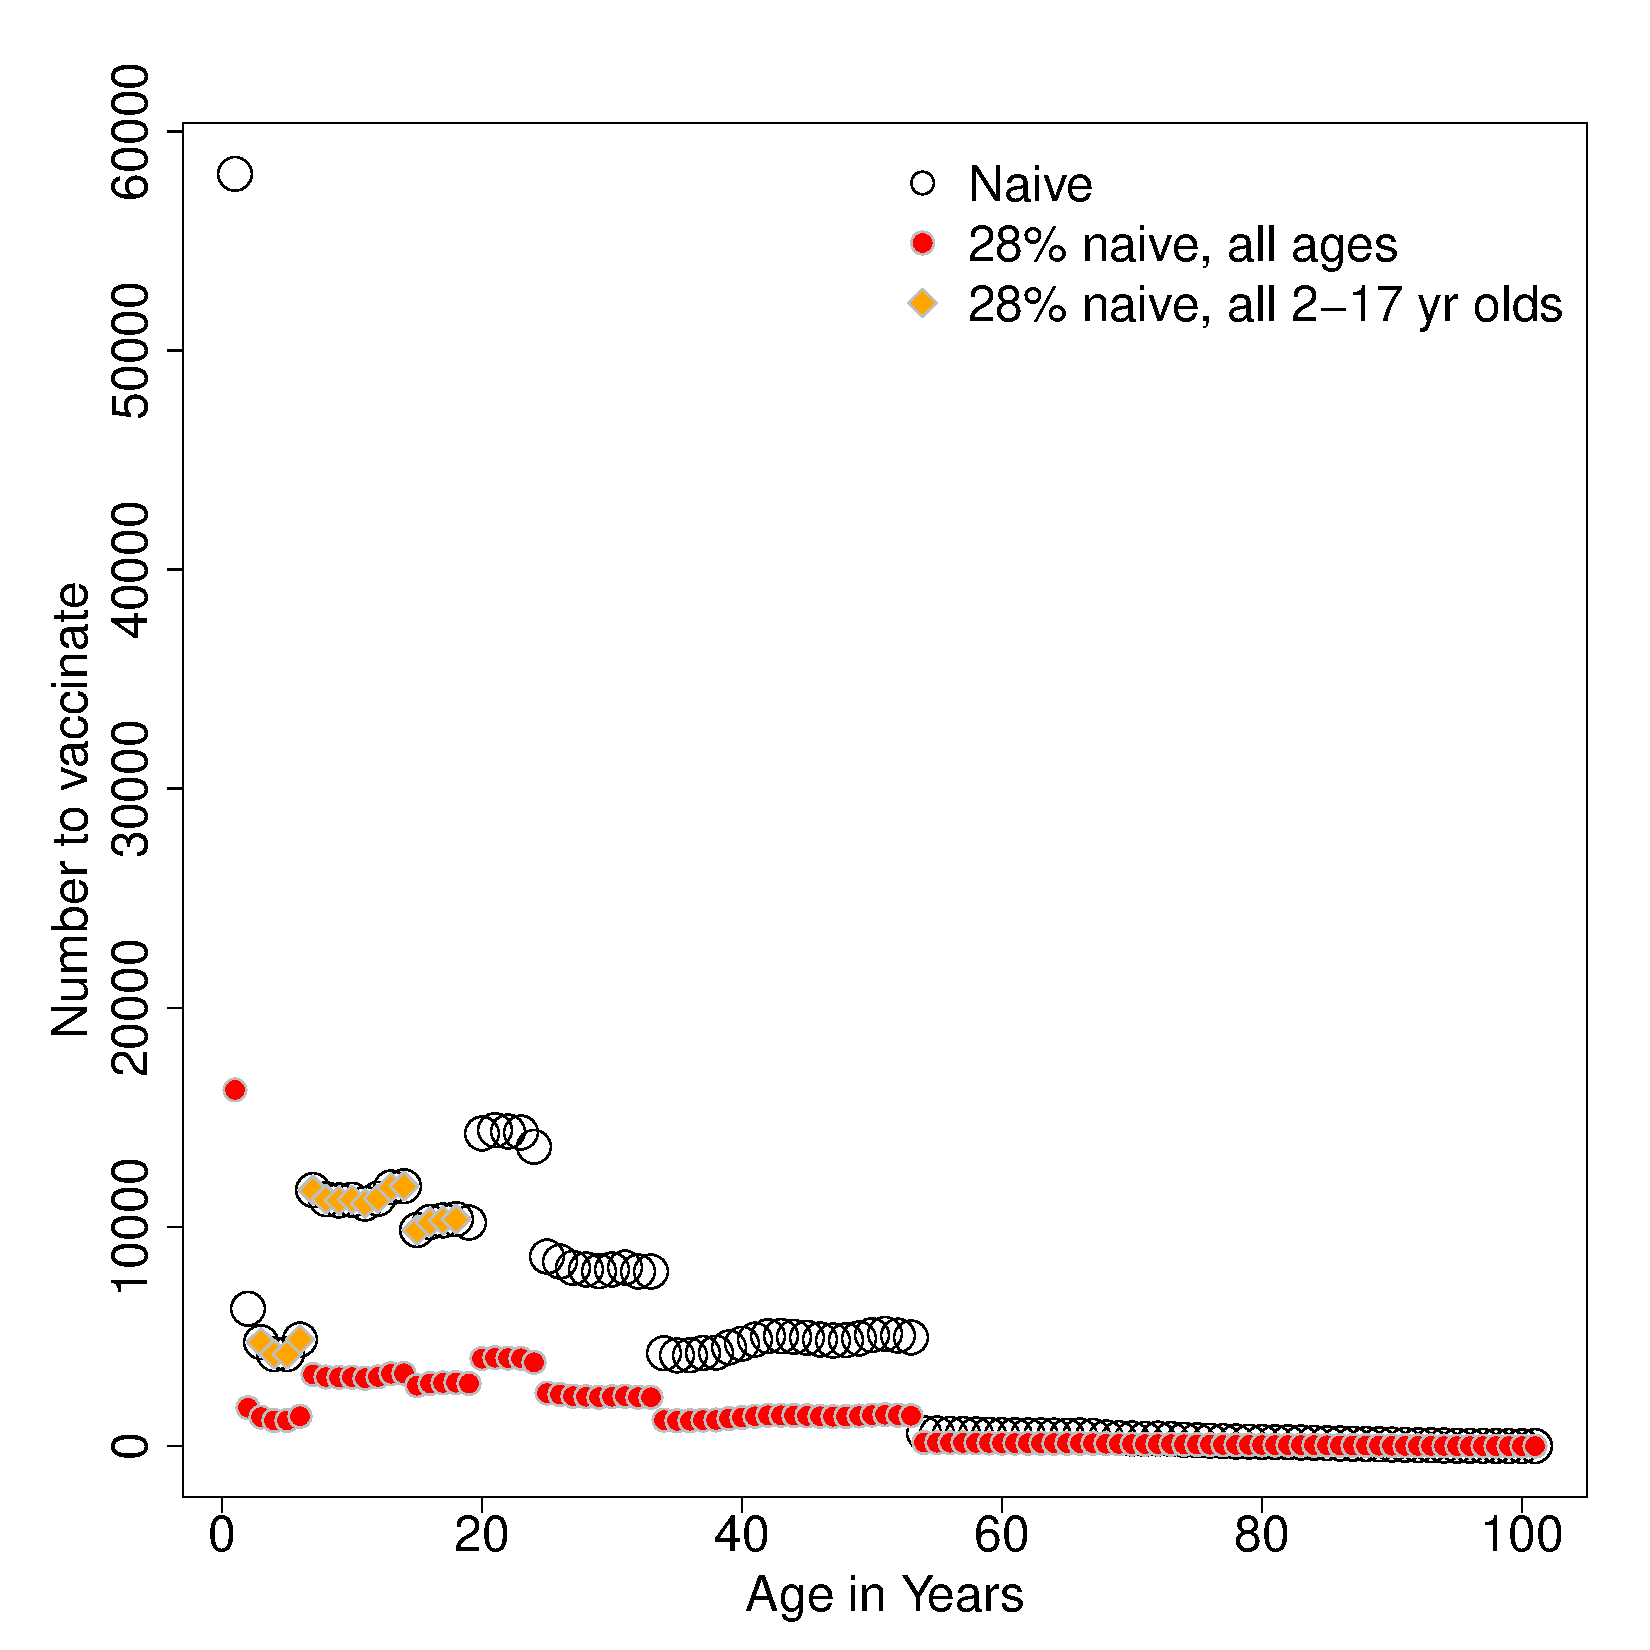
\includegraphics{draftfinalreport-061}
\end{center}
\caption{Age and vaccination status of cases}
\label{fig:ageandvac}
\end{figure}

\begin{figure}[h!]
\begin{center}
\includegraphics{draftfinalreport-062}
\end{center}
\caption{Age of vaccination of vaccinated measles cases}
\label{fig:vaccstat}
\end{figure}



\subsection{Benefit--cost analysis discussion}
The results presented here are based on available data, and only a 10 week period for the 2013--2014 outbreak. The majority of the cost analyses were discussed in our previous interim report and though some details have changed, we will focus here on the benefit--cost analyses. However, for all analyses more detailed costs of all aspects of hospitalisation would be beneficial. So too would information of the cost of measles vaccination in New Zealand.

We have used standard discounting from healthcare of 3\% per annum \citep{honeycutt6}, but again there may be official New Zealand discounting rates that we are unaware of.
For our benefit--cost analyses we have not included measles outbreak management costs, though these were provided for the period of January 1 -- March 9, 2014 (Table ~\ref{table:direct}). Including these could be done, but we would like some further data of these before including them in our benefit--cost analyses. It is likely to be unrealistic to assume that these costs would be linearly related with the number of measles cases, making it difficult to extrapolate these costs outside the reported period for 2014.

In other nations' outbreaks, the average cost per measles case was estimated to be US\$254, US\$276, and US\$307 for Canada, the Netherlands, and the UK, respectively \citep{carabin2}. In our analyses if we include loss of earnings and hospitalisation costs, our estimates are higher, around US\$959 per case. This figure is from NZ\$ 852 for loss of wages and 0.17 * NZ \$ 1710 for costs related to attending hospital. However, costs can vary widely, with the containment of a single case and two secondary cases of measles in 2004 in Iowa, USA, estimated to cost US\$142,542 alone \citep{dayan5}.

Our estimates for the benefit--cost ratio of catch up vaccination are also much higher than those in some studies, if we presume the $R_v$ is greater than 1 and measles will continue to circulate among the presently naive and susceptible New Zealand population until everyone has been infected. Estimates in Korea suggest catch up vaccination schemes have a benefit--cost ratio of just over one \citep{bae13}. However, if we presume that in a totally naive population $R_0$ for measles is around 12, and sometimes estimated to be more than 18 (i.e. 1 case infects 18 others on average, \citep{anderson91}) then the majority of naive people becoming infected is not unrealistic given some of our $R_v$ estimates (Figure~\ref{fig:r0}). The benefits of catch up vaccination are clear once $R_v$ is greater than one (Table~\ref{tab:cost_sim}). If measles continues to cause smaller outbreaks, and/or $R_v$ is less than one (Figure~\ref{fig:r0}), then there is little financial benefit in additional vaccination (Table~\ref{tab:cost_sim} and Table~\ref{tab:cost_ave}), though there may be medical and other benefits relating to maintaining measles free status that we have not included in our report.

Finally, our model of measles introductions is a simple one, and more complex models may predict smaller outbreaks depending on contact structure and other scenarios, such as the size of the local naive population. The spatial effects of measles transmission may have affected both our multivariate regression analyses (Section~\ref{sub:risk_analyses}) and will affect the predictions from modelling exercises (Section~\ref{sec:epidemic_modelling}). Whatever happens, however, it is clear that there will be ongoing costs to maintain New Zealand free of endemic measles and introductions occurring on an annual basis (see previous report) may produce some large and costly outbreaks, even if vaccination cover is high and $R_v$ is less than one (Figure~\ref{fig:sim} and Figure ~\ref{fig:sim1}).

\subsection{Cost analysis summary}


\begin{itemize}
\item Our initial estimates suggest the ongoing 2013--2014 measles outbreak has cost New Zealand over \$750,000.
\end{itemize}

\subsection{Benefit--cost analysis summary}
\begin{itemize}
\item The mean wage losses per measles case is estimated to be \$852
\item The mean cost per measles case attending hospital is estimated to be \$1710
\item Approximately 17\% of measles cases attend hospital
\item For $R_v$ values estimated for the 2013--2014 outbreak and the upper bounds estimated for all outbreaks since 2009, the benefits of catch up vaccination strategies are clear (>1 B/C ratio).
\item For $R_v$ values at the lower bounds of the estimates for all outbreaks since 2009, the benefits of catch up vaccination strategies are not clear and may not be cost effective (<1 B/C ratio).
\item Large outbreaks, with a mean size of approximately 151 cases per year, median of 2, but peak size of up to many thousands, may occur regularly due to importation, despite $R_v$ being below one and the epidemic predicted to die out without additional interventions.
\end{itemize}

\subsection{Future cost-benefit analyses}
Using the results above we aim to:
\begin{itemize}
\item Estimate the costs and benefits for targeted vaccination, based either on the univariate analyses presented to date in the \emph {Progress Towards Measles Elimination in New Zealand - Final} report or adjusted if any additional risk groups are identified in the multivariate analyses (section~\ref{sub:risk_analyses}) or modelling (section~\ref{sec:epidemic_modelling}).
\end{itemize}

We also require additional clarifications of the data, regarding:
\begin {itemize}
\item What hospital costs refer to, such as if a hospital day were 0 does that mean the case stayed in the hospital but not overnight? Or, does it mean the case stayed for less than 24 hours?
\end {itemize}
Once more complete data are available, comparisons of these results will be made to other published studies, discussed above.


\section {Summary of key findings}
\begin{itemize}
\item New Zealand is at risk of frequent measles importation due to travel and endemic measles elsewhere in the world.
\item The cost of the current measles outbreak is estimated to be at least \$750,000.
\item Analyses of outbreak data suggest that measles $R_v$ values often include 1 and in this year, 2014, are well above one. This analysis suggests improved vaccination is a requisite to prevent measles becoming endemic again.
\item Risk of measles infection decreases significantly with age
\item Pacific people are statistically more at risk on a per capita basis, as are those living in better socio-economic situations
\item Pacific and Asian children in the 6--17 year age categories have been at lower risk of measles than European or Maori children of the same age
\item Additional vaccination levels to push $R_v$ below one among the currently naive population in New Zealand range from 0\% ($R_v$ < 1) to 53\% ($R_v$ 2.13, upper 95\% confidencelimit 2013--2014 outbreak, approximately 250,000 vaccinations), depending on the appropriate reproduction number, $R_v$, for measles in New Zealand.
\item The mean wage losses per measles case is estimated to be \$852
\item The mean cost per measles case attending hospital is estimated to be \$1710, and approximately 17\% of measles cases attend hospital
\item For $R_v$ values estimated for the 2013--2014 outbreak and the upper bounds estimated for all outbreaks since 2009, the benefits of catch up vaccination strategies are clear (>1 B/C ratio).
\item For $R_v$ values at the lower bounds of the estimates for all outbreaks since 2009, the benefits of catch up vaccination strategies are not clear and may not be cost effective (<1 B/C ratio).
\item Large outbreaks, with a mean size of approximately 151 cases per year, median of 2, but peak size of up to many thousands, may occur regularly due to importation, despite $R_v$ being below one and the epidemic predicted to die out without additional interventions.
\end{itemize}



\section{Acknowledgments}
The authors wish to thank Tomasz Kiedrzynski, Lisa Oakley and Nic Aagaard from the Ministry of Health, Ruth Pirie and colleagues from ESR, and June Atkinson from University of Otago for help in obtaining the appropriate materials for analyses.

\begin{thebibliography}{}
\bibliographystyle{plain}

\bibitem[Agur et al.(1993)]{agur93}
Agur, Z., L. Cojocaru, G. Mazor, R.~M. Anderson and Y.~L. Danon (1993).
\newblock Pulse mass measles vaccination across age cohorts.
\newblock \emph{Proceedings of the National Academy of Sciences USA}, 90, 11698--11702.

\bibitem[Anderson and May(1991)]{anderson91}
Anderson, R.~M. and R.~M. May (1991).
\newblock \emph{Infectious diseases of humans: dynamics and control}. Oxford: Oxford University Press.

\bibitem[Anon.(2002a)]{anon2a}
Anon. (2002a).
\newblock \emph{Immunisation handbook}
\newblock Wellington: Ministry of Health. pp.~131--146.

\bibitem[Anon.(2002b)]{anon2b}
Anon. (2002b).
\newblock \emph{Infectious diseases in livestock}
\newblock The Royal Society. pp.~68.

\bibitem[Babad et al.(1995)]{babad95}
Babad, H.~R., D.~J. Nokes, N.~J. Gay, E. Miller, P. Morgan-Capner, and R.~M. Anderson (1995).
\newblock Predicting the impact of measles vaccination in England and Wales: model validation and analysis of policy options.
\newblock \emph{Epidemiology and Infection}, 114, 319--344.

\bibitem[Bae et al.(2013)]{bae13}
Bae, G.~R, Y.~J. Choe, U.~Y. Go, Y.~I. Kim, and J.~K. Lee (2013). 
\newblock Economic analysis of measles elimination program in the Republic of Korea, 2001: A cost benefit analysis study.
\newblock \emph {Vaccine}, 31, 2661--2666.

\bibitem[Carabin et al.(2002)]{carabin2}
Carabin, H., W.~J. Edmunds, U. Kou, S. van den Hof, and V.~H. Nguyen (2002). 
\newblock Measles in industrialized countries: a review of the average costs of adverse events and measles cases.
\newblock \emph{BMC Public Health}, 2, 22.

\bibitem[Carabin et al.(2003)]{carabin3}
Carabin, H., W.~J. Edmunds, M. Gyldmark, P. Beutels, D. Levy-Bruhl, H. Salo, U.~K. and Griffiths (2003)
\newblock The cost of measles in industrialised countries.
\newblock \emph{Vaccine}, 21,4167--4177.

\bibitem[Clements and Hussey(2004]{clements4}
Clements, C.~J. and G.~D. Hussey (2004).
\newblock Chapter 4: Measles.
\newblock In \emph{The Global Epidemiology of Infectious Diseases},  Murray, C., A.~D. Lopez, and C.~D. Mathers, (eds.), Geneva.
World Health Organization, pp.~391.

\bibitem[Coleman et al.(2012)]{coleman12}
Coleman, M.~S., L. Garbat-Welch, H. Burke, M. Weinberg, K. Humbaugh, A. Tindall, and J. Cambron (2012).
\newblock Direct costs of a single case of refugee-imported measles in Kentucky.
\newblock \emph{Vaccine}, 30,317--321.

\bibitem[Dayan et al.(2005)]{dayan5}
G.~H. Dayan, I.~R. Ortega-Sanchez, C.~W. LeBaron, M.~P. Quinlisk, and the Iowa Measles Response Team (2005).
\newblock The cost of containing one case of measles: the economic impact on the public health infrastructure - Iowa, 2004.
\newblock \emph{Pediatrics}, 116:e1; DOI:10/1542/peds.2004-2512.

\bibitem[Diekmann et al.(2000)]{diekmann0}
Diekmann, O. and  J.~A.~P. Heesterbeek (2000).
\newblock \emph{Mathematical epidemiology of infectious diseases: model building, analysis and interpretation}.
Chichester: Wiley.

\bibitem[Diekmann et al.(2013)]{diekmann13}
Diekmann, O.,  J.~A.~P. Heesterbeek, and T. Britton (2013).
\newblock \emph{Mathematical tools for understanding infectious disease dynamics}.
Princeton: Princeton University Press.

\bibitem[Edmunds et al.(2000)]{edmunds0}
Edmunds, W.~J., N.~J. Gay, M. Kretzschmar, R.~G. Pebody and H. Wachman (2000).
\newblock The pre-vaccination epidemiology of measles, mumps and rubella in Europe: implications for modelling studies.
\newblock \emph{Epidemiology and Infection}, 125, 635--650.

\bibitem[Filia et al.(2007)]{filia7}
Filia, A., A. Brenna, A. Pana, G.~M. Cavallaro, M. Massari and M.~L.C. degli Atti (2007).
\newblock Health burden and economic impact of measles-related hospitalization in Italy, 2002-2003.
\newblock \emph{BMC Public Health}, 7,169

\bibitem[Flego et al.(2013)]{flego13}
Flego, K.~L., D.~A. Belshaw, V. Sheppeard, and K.~M. Weston (2013).
\newblock Impacts of a measles outbreak in western Sydney on public health resources.
\newblock \emph{Communicable Diseases Intelligence Quarterly Report}, 37, E240--245.

\bibitem[Gay et al.(1998)]{gay98}
Gay, N.~J., L. Pelletier, and P. Duclos (1998).
\newblock Modelling the incidence of measles in Canada: an assessment of the options for vaccination policy.
\newblock \emph{Vaccine}, 16, 794--801.

\bibitem[Glass et al.(2004)]{glass4}
Glass, K., J. Kappey, and B.~T. Grenfell (2004).
\newblock The effect of heterogeneity in measles vaccination population immunity.
\newblock \emph{Epidemiology and Infection}, 132, 675--683.

\bibitem[Honeycutt et al.(2006)]{honeycutt6}
Honeycutt, A. A., L. Clayton, O. Khavjou, E.~A. Finkelstein, M. Prabhu, J.~L. Blitstein, W. Dougles Evans, and J.~M. Renaud (2006).
\newblock Guide to Analyzing the Cost-Effectiveness of Community Public Health Prevention Approaches.
http://aspe.hhs.gov/health/reports/06/cphpa/report.pdf

\bibitem[Klinkenberg et al.(2011)]{klinkenberg11}
Klinkenberg, D. and H. Nishiuraa (2011).
\newblock The correlation between infectivity and incubation period of measles, estimated from households with two cases.
\newblock \emph{Journal of Theoretical Biology},284, 52--60

\bibitem[Koopmanschap(1998)]{koopmanschap98}
Koopmanschap, M.~A. (1998).
\newblock Cost-of-illness studies: useful for health policy?
\newblock \emph{Pharmacoeonomics}, 14, 143--148.

\bibitem[Larg and Moss(2011)]{larg11}
Larg, A. and J.~R. Moss (2011).
\newblock Cost-of-illness studies: a guide to critical evaluation.
\newblock \emph{Pharmacoeconomics}, 29,653--671.

\bibitem[Mansoor et al.(1998)]{mansoor98}
Mansoor, O., A. Blakely, M. Baker, M. Tobias, and A. Bloomfield (1998).
\newblock A measles epidemic controlled by immunisation. 
\newblock \emph{New Zealand Medical Journal}, 111, 467--471.

\bibitem[Ortega-Sanchez et al.(2014)]{ortegasanchez14}
Ortega-Sanchez, I.~R., M. Vijayaraghavan, A.~E. Barskey, and G.~S. Wallace (2014).
\newblock The economic burden of sixteen measles outbreaks on United States public health departments in 2011.
\newblock \emph{Vaccine}, 32,1311--1317.

\bibitem[Obidia et al.(2012)]{obidia12}
Obadia, T., R. Haneef and P--Y. Boelle
\newblock The R0 package: a toolbox to estimate reproduction numbers for epidemic outbreaks.
\newblock \emph{BMC Medical Informatics and Decision Making}, 2012, 12--147.

\bibitem[Parker et al.(2006)]{parker6}
Parker, A.~A., W. Staggs, G.~H. Dayan, I.~R. Ortega-Sanchez, P.~A. Rota, L. Lowe, P. Boardman, R. Teclaw, C. Graves, and C.~W. LeBaron (2006).
\newblock Implications of a 2005 measles outbreak in Indiana for sustained elimination of measles in the United States.
\newblock \emph{The New England Journal of Medicine}, 355, 447--455.

\bibitem[Prouty et al.(2001)]{prouty1}
Prouty, R.W., G. Smith and K.~C. Lakin (2001).
\newblock Residential services for persons with developmental disabilities: status and trends through 2000.
\newblock \emph{Minneapolis: Institute on Community Integration}, University of Minnesota, pp.~179, rtc.umn.edu/risp00.

\bibitem[Roberts(2004)]{roberts4}
Roberts, M. (2004).
\newblock A mathematical model for measles vaccination.
\newblock Wellington: Ministry of Health.

\bibitem[Roberts and Tobias(2000)]{roberts0}
Roberts, M.~G. and M.~I. Tobias (2000).
\newblock Predicting and preventing measles epidemics in New Zealand: Application of a mathematical model. 
\newblock \emph{Epidemiology and Infection}, 124, 279--287.

\bibitem[Saha and Gerdtham(2013)]{saha13}
Saha, S. and U.~G. Gerdtham (2013).
\newblock Cost of illness studies on reproductive, maternal, newborn, and child health: a systematic literature review.
\newblock \emph{Health Economics Review}, doi:10.1186/2191-1991-3-24.

\bibitem[Siedler et al.(2006)]{siedler6}
Siedler, A., A. Tischer, A. Mankertz, and S. Santibanez (2006).
\newblock Two outbreaks of measles in Germany 2005.
\newblock \emph{Eurosurveillance} 2006:11(4) article 5, \href{http://www.eurosurveillance.org/ViewArticle.aspx?ArticleId=615}{www.eurosurveillance.org}, accessed 14 June 2014.

\bibitem[Stack et al.(2011)]{stack11}
Stack, M.~L., S. Ozawa, D.~M. Bishai, A. Mirelman, Y. Tam, L. Niessen, D.~G. Walker, and O.S. Levine (2011).
\newblock Estimated economic benefits during the 'decade of vaccine' include treatment savings, gains in labor productivity.
\newblock \emph{Health Affairs}, 30,1021--1028.

\bibitem[Statistics New Zealand(2014))]{stats14}
\newblock \emph{Statistics New Zealand} (2014).
http://nzdotstat.stats.govt.nz/, accessed 17 June 2014.

\bibitem[Tobias and Roberts(1998)]{tobias98}
Tobias, M.~I. and M.~G. Roberts (1998).
\newblock Predicting and preventing measles epidemics in New Zealand: Application of a mathematical model.
\newblock Wellington: Ministry of Health.

\bibitem[Wallinga et al.(2001)]{wallinga1}
Wallinga, J., D. Levy-Bruhl, N.~J. Gay, and C.~H. Wachman (2001).
\newblock Estimation of measles reproduction ratios and prospects for elimination of measles by vaccination in some Western European countries.
\newblock \emph{Epidemiology and Infection}, 127, 281--295.

\bibitem[Wallinga and Teunis(2004)]{wallinga4}
Wallinga, J., and P. Teunis (2004).
\newblock Different Epidemic Curves for Severe Acute Respiratory Syndrome Reveal Similar Impacts of Control Measures.
\newblock \emph{American Journal of Epidemiology}, 160, 509.

\bibitem[Wichmann et al.(2009)]{wichmann9}
Wichmann, O., A. Siedler, D. Sagebiel, W. Hellenbrand, S. Santibanez, A. Mankertz, G. Vogt, U. van Treeck, and G. Krause (2009).
\newblock Further efforts needed to achieve measles elimination in Germany: results of an outbreak investigation.
\newblock \emph{Bulletin of the World Health Organization}, 87, 108--115.

\bibitem[Wolfson et al.(2007)]{wolfson7}
Wolfson, L.~J., P.~M. Strebel, M. Gacic-Dobo, E.~J. Hoekstra, J.~W. McFarland, and B.~S. Hersh (2007).
\newblock Has the 2005 measles mortality reduction goal been achieved? A natural history modelling study.
\newblock \emph{Lancet}, 369, 191--200.

\bibitem[WHO(2013)]{who13}
World Health Organisation measles media centre, January (2013)
\newblock Geneva: World Health Organization.
\href{http://www.who.int/mediacentre/news/notes/2013/measles_20130117/en/}{www.who.int}, accessed July 1, 2014.

\bibitem[Zhou et al.(2004)]{zhou4}
Zhou, F, S. Reef, M. Massoudi, M.~J. Papania, H.~R. Yusuf, B. Bardenheier, L. Zimmerman, and M.~M. McCauley (2004).
\newblock An economic analysis of the current universal 2-dose measles-mumps-rubella vaccination program in the United States.
\newblock \emph{Journal of Infectious Diseases}, 189, S131--45.

\end{thebibliography}

\end{document}
